\documentclass[11pt,a4paper]{article}
\pdfoutput=1
\usepackage{jinstpub}         
%\usepackage{Styles/jinstpub} %%%% Comment previous line and comment uncomment this line if using pdflatex from terminal



\newif\ifshowcomments
%%%%%%%%%%%%%%%%%%%%%%%%%%%%%%%%%%%%%%%%%%%%%%%%%%%%%%%%%%%%%%%%%%%%%%%%
%%% TO HIDE COMMENTS, FOLLOWING LINE SHOULD BE \showcommentsfalse, 
%%% OTHERWISE \showcommentstrue
%%%%%%%%%%%%%%%%%%%%%%%%%%%%%%%%%%%%%%%%%%%%%%%%%%%%%%%%%%%%%%%%%%%%%%%
\showcommentstrue
\ifshowcomments
\newcommand{\CD}[1]{\textcolor{purple}{CD: #1}}
\newcommand{\BS}[1]{\textcolor{blue}{BS: #1}}
\else
\newcommand{\CD}[1]{}
\newcommand{\BS}[1]{}
\fi 

\usepackage[colorinlistoftodos]{todonotes}


\usepackage{epsfig}
\usepackage{amssymb}
\usepackage{subfigure}
\usepackage{lineno}
\linenumbers

\usepackage{titlesec}
\titleformat{\paragraph}[runin]
{\bfseries\scshape}{\theparagraph}{1em}{}
\setcitestyle{square}

\RequirePackage{xspace}

\def\icemc {\texttt{icemc}\xspace}


%%%%%%%%%%%%%%%%%%%%%%%%%%%%%%%%%%%%%%%%%%%%%%%
%%%%%%%%%%%%%%%%%   LEPTONS   %%%%%%%%%%%%%%%%%
%%%%%%%%%%%%%%%%%%%%%%%%%%%%%%%%%%%%%%%%%%%%%%%
\let\emi\en
\def\electron   {\text{e}\xspace}
\def\en         {\ensuremath{\text{e}^-}\xspace}  
\def\ep         {\ensuremath{\text{e}^+}\xspace}
\def\epm        {\ensuremath{\text{e}^\pm}\xspace} 
\def\epem       {\ensuremath{\text{e}^+\text{e}^-}\xspace}
\def\ee         {\ensuremath{\text{e}^-\text{e}^-}\xspace}

\def\mmu        {\ensuremath{\mu}\xspace}
\def\mup        {\ensuremath{\mu^+}\xspace}
\def\mun        {\ensuremath{\mu^-}\xspace} 
\def\mumu       {\ensuremath{\mu^+\mu^-}\xspace}
\def\mtau       {\ensuremath{\tau}\xspace}

\def\taup       {\ensuremath{\tau^+}\xspace}
\def\taum       {\ensuremath{\tau^-}\xspace}
\def\tautau     {\ensuremath{\tau^+\tau^-}\xspace}

\def\ellm       {\ensuremath{\ell^-}\xspace}
\def\ellp       {\ensuremath{\ell^+}\xspace}
\def\ellell     {\ensuremath{\ell^+ \ell^-}\xspace}

\def\nub        {\ensuremath{\overline{\nu}}\xspace}
\def\nunub      {\ensuremath{\nu{\overline{\nu}}}\xspace}
\def\nub        {\ensuremath{\overline{\nu}}\xspace}
\def\nunub      {\ensuremath{\nu{\overline{\nu}}}\xspace}
\def\nue        {\ensuremath{\nu_{\text{e}}}\xspace}
\def\nueb       {\ensuremath{\nub_{\text{e}}}\xspace}
\def\nuenueb    {\ensuremath{\nue\nueb}\xspace}
\def\num        {\ensuremath{\nu_\mu}\xspace}
\def\numb       {\ensuremath{\nub_\mu}\xspace}
\def\numnumb    {\ensuremath{\num\numb}\xspace}
\def\nut        {\ensuremath{\nu_\tau}\xspace}
\def\nutb       {\ensuremath{\nub_\tau}\xspace}
\def\nutnutb    {\ensuremath{\nut\nutb}\xspace}
\def\nul        {\ensuremath{\nu_\ell}\xspace}
\def\nulb       {\ensuremath{\nub_\ell}\xspace}
\def\nulnulb    {\ensuremath{\nul\nulb}\xspace}

\def\p          {\text{p}\xspace}
\def\n          {\text{n}\xspace}


\def\km2str     {\ensuremath{\,\text{km}^2\text{str}}\xspace}
\def\km3str     {\ensuremath{\,\text{km}^3\text{str}}\xspace}

\newcommand{\tev}{\ensuremath{\mathrm{\,Te\kern -0.1em V}}\xspace}
\newcommand{\gev}{\ensuremath{\mathrm{\,Ge\kern -0.1em V}}\xspace}
\newcommand{\mev}{\ensuremath{\mathrm{\,Me\kern -0.1em V}}\xspace}
\newcommand{\kev}{\ensuremath{\mathrm{\,ke\kern -0.1em V}}\xspace}
\newcommand{\ev}{\ensuremath{\mathrm{\,e\kern -0.1em V}}\xspace}
\newcommand{\evv}{\ensuremath{\mathrm{\,e\kern -0.1em V}^2}\xspace}
\newcommand{\gevc}{\ensuremath{{\mathrm{\,Ge\kern -0.1em V\!/}c}}\xspace}
\newcommand{\mevc}{\ensuremath{{\mathrm{\,Me\kern -0.1em V\!/}c}}\xspace}
\newcommand{\gevcc}{\ensuremath{{\mathrm{\,Ge\kern -0.1em V\!/}c^2}}\xspace}
\newcommand{\mevcc}{\ensuremath{{\mathrm{\,Me\kern -0.1em V\!/}c^2}}\xspace}
\newcommand{\evcc}{\ensuremath{{\mathrm{\,e\kern -0.1em V\!/}c^2}}\xspace}
\newcommand{\evvcccc}{\ensuremath{{\mathrm{\,e\kern -0.1emV^2\!/}c^4}}\xspace}

\newcommand{\effarea}{\ensuremath{\langle A\Omega\rangle(E)}\xspace}
\newcommand{\effvol}{\ensuremath{\langle V\Omega\rangle(E)}\xspace}

\newcommand{\degree}{\ensuremath{^{\circ}}}

\date{\today}

\title{\icemc: A Monte Carlo Simulation for Cosmogenic Neutrinos interacting in the Antarctic ice as viewed by the Antarctic Impulsive Transient Antenna (ANITA)}

\collaboration{ANITA Collaboration}


\affiliation[uc]{Dept. of Physics, Enrico Fermi Inst., Kavli Inst. for Cosmological Physics, Univ. of Chicago , Chicago, IL 60637.}
\affiliation[ucla]{Dept. of Physics and Astronomy, Univ. of California, Los Angeles, Los Angeles, CA 90095.}
\affiliation[osu]{Dept. of Physics, Center for Cosmology and Particle Astrophysics, Ohio State Univ., Columbus, OH 43210.}
\affiliation[uh]{Dept. of Physics and Astronomy, Univ. of Hawaii, Manoa, HI 96822.}
\affiliation[ntu]{Dept. of Physics, Grad. Inst. of Astrophys.,\& Leung Center for Cosmology and Particle Astrophysics, National Taiwan University, Taipei, Taiwan.}
\affiliation[ku]{Dept. of Physics and Astronomy, Univ. of Kansas, Lawrence, KS 66045.}
\affiliation[mephi]{National Research Nuclear University, Moscow Engineering Physics Institute, 31 Kashirskoye Highway, Russia 115409.}
\affiliation[wu]{Dept. of Physics and McDonnell Center for the Space Sciences, Washington Univ. in St. Louis, MO 63130.}
\affiliation[slac]{SLAC National Accelerator Laboratory, Menlo Park, CA, 94025.}
\affiliation[ud]{Dept. of Physics, Univ. of Delaware, Newark, DE 19716.}
\affiliation[ucl]{Dept. of Physics and Astronomy, University College London, London, United Kingdom.}
\affiliation[jpl]{Jet Propulsion Laboratory, Pasadena, CA 91109.}
\affiliation[ccap]{Center for Cosmology and Particle Astrophysics, Ohio State Univ., Columbus, OH 43210.}
\affiliation[calpoly]{Physics Dept., California Polytechnic State Univ., San Luis Obispo, CA 93407.}
\affiliation[mpl]{Max-Planck-Institut f\"{u}r Kernphysik, 69117 Heidelberg, Germany.}
\affiliation[brus]{Astrophysical Institute, Vrije Universiteit Brussel, Pleinlaan 2, 1050, Brussels, Belgium.}
\affiliation[lsst]{LSST, 950 North Cherry Avenue, Tucson, AZ 85721}
\affiliation[ucsd]{Center for Astrophysics and Space Sciences, Univ. of California, San Diego, La Jolla, CA 92093}


\author[osu]{P.~Allison}
\author[osu]{O.~Banerjee}
\author[ucl]{L.~Batten} 
\author[osu]{J.~J.~Beatty} 
\author[uc,lsst]{K.~Bechtol}
\author[jpl]{K.~Belov}
\author[ku,mephi]{D.~Z.~Besson}
\author[wu]{W.~R.~Binns} 
\author[wu]{V.~Bugaev} 
\author[ud]{P.~Cao} 
\author[ntu]{C.~C.~Chen} 
\author[ntu]{C.~H.~Chen}
\author[ntu]{P.~Chen} 
\author[ud]{J.~M.~Clem} 
\author[osu]{A.~Connolly} 
\author[ucl]{L.~Cremonesi} 
\author[osu]{B.~Dailey} 
\author[uc]{C.~Deaconu} 
\author[wu]{P.~F.~Dowkontt} 
\author[uh]{B.~D.~Fox} 
\author[osu]{J.~W.~H.~Gordon}
\author[uh]{P.~W.~Gorham} 
\author[uh]{B.~Hill} 
\author[ntu]{J.~J.~Huang}
\author[osu]{R.~Hupe} 
\author[wu]{M.~H.~Israel} 
\author[jpl]{K.~M.~Liewer}
\author[ntu]{S.~Y.~Lin}
\author[ntu]{T.~C.~Liu} 
\author[uc]{A.~Ludwig} 
\author[uh]{L.~Macchiarulo} 
\author[uh]{S.~Matsuno} 
\author[osu]{K.~McBride}
\author[uh]{C.~Miki} 
\author[ud,brus]{K.~Mulrey}
\author[ntu]{J.~Nam}
\author[ucl]{R.~J.~Nichol}
\author[ku,mephi]{A.~Novikov} 
\author[uc]{E.~Oberla} 
\author[osu]{S.~Prohira}
\author[wu]{B.~F.~Rauch}
\author[uh,ucsd]{J.~M.~Roberts}
\author[jpl]{A.~Romero-Wolf}
\author[uh]{B.~Rotter}
\author[uh]{J.~W.~Russell} 
\author[ucla]{D.~Saltzberg}
\author[ud]{D.~Seckel}
\author[uh,mpl]{H.~Schoorlemmer}
\author[ntu]{J.~Shiao}
\author[osu]{S.~Stafford}
\author[ku]{J.~Stockham}
\author[ku]{M.~Stockham}
\author[ucla]{B.~Strutt} 
\author[calpoly]{J.~Stuhr}
\author[uh]{G.~S.~Varner}
\author[uc]{A.~G.~Vieregg}
\author[ntu]{S.~H.~Wang}
\author[calpoly]{S.~A.~Wissel}


\abstract{A Monte Carlo simulation tool for the radio detection of Ultra High Energy (UHE) neutrino interactions in the Antarctic ice, \icemc, is described in this article.
This tool includes the simulation of ultra high energy neutrinos, the parametrization of the Askaryan radiation generated by their interaction in the ice, the propagation of the radiation through ice and air to a simulated model of the third and fourth ANITA (Antarctic Impulsive Transient Antenna) flights.
This paper provides an overview of the \icemc simulation, a detailed description of the physics models used, data/simulation comparisons to validate the physics performance, and a summary of the impact of published results. Finally the sensitivity of the fourth ANITA flight is presented. If no neutrinos are detected ANITA is expected to improve upon its world leading limit on the cosmogenic neutrino flux above $10^{19}$\,eV.}

\keywords{neutrino radio detection, ultra-high-energy, Monte Carlo}

\arxivnumber{...}

\begin{document}

\maketitle

\flushbottom

\section{Introduction}
The ANtarctic Impulsive Transient Antenna (ANITA) experiment is a NASA-funded, balloon-borne experiment aiming primarily to detect Ultra-High-Energy (UHE) neutrinos and cosmic rays~\cite{ANITA1detector,ANITA1paper,ANITA2paper,ANITA2erratum}.
UHE neutrinos may be produced when cosmic rays interact with the
cosmic microwave background, either through the Greisen Zatsepin
Kuzmin (GZK)~\cite{greisen1966end,zatsepin1966gt} mechanism or through photo-disintegration, or directly from an astrophysical source.
UHE neutrinos interact in the Antarctic ice and produce a coherent radio pulse of Askaryan radiation~\cite{askaryan}. UHE cosmic rays interact with the geomagnetic field to produce a coherent radio impulse~\cite{suprun2003synchrotron,falcke2003detecting,ANITA1UHECR}. The geometry of the Earth's magnetic field in Antarctica allows ANITA to distinguish the signatures of these two types of events through their polarization.

The ANITA experiment flies approximately 40\,km above Antarctica looking for radio signals in the band between 200 and 1200\,MHz, produced by UHE neutrinos and cosmic rays.
Figure~\ref{fig:intro_ANITAconcept} shows a basic scheme of the
Askaryan neutrino detection at the ANITA experiment, as well as the UHE cosmic ray detection principle.
Four ANITA flights (Section~\ref{sec:anita3}) have been successfully
completed as of 2019, and this paper focuses on the simulations of the third and fourth ANITA flights.

\begin{figure}[!h]\centering
  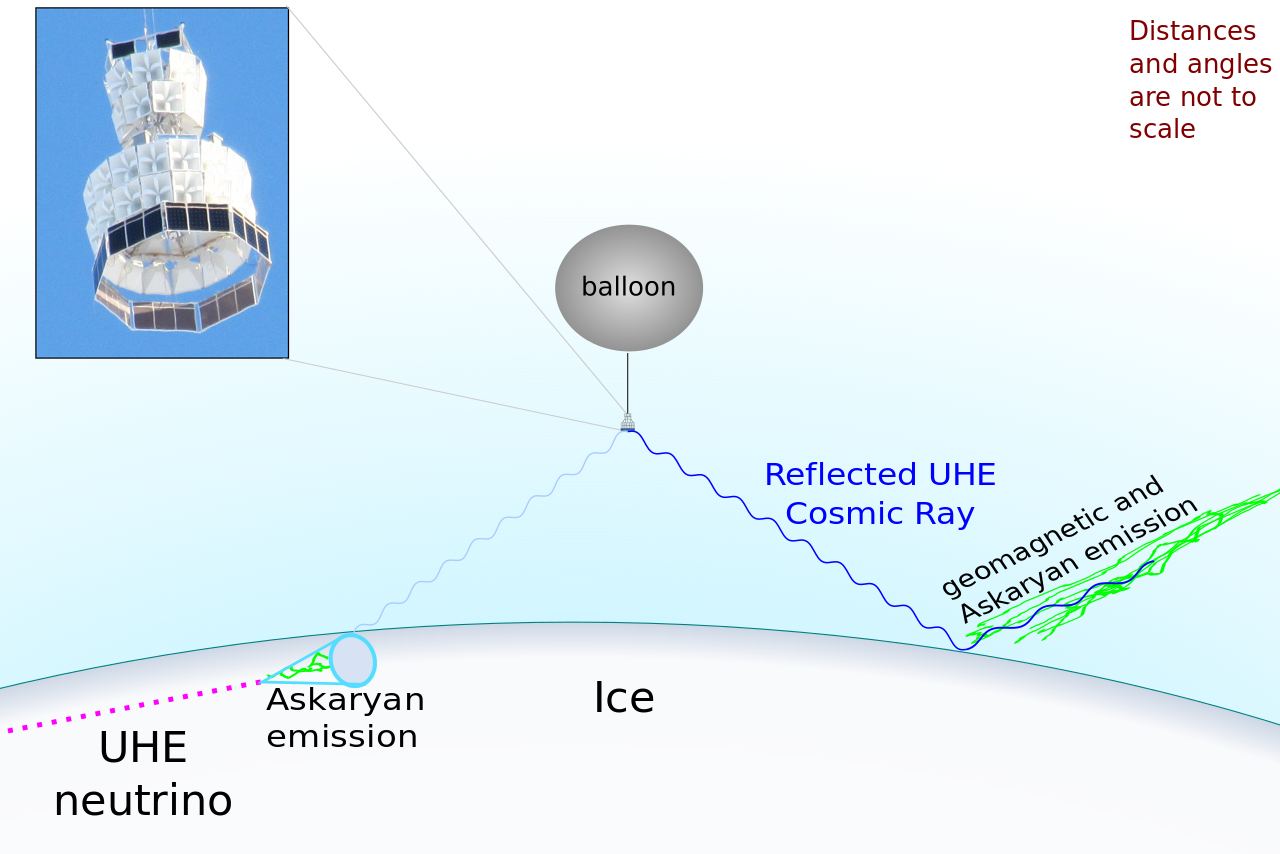
\includegraphics[width=.8\linewidth]{./Figs/ANITA_scheme_icemcpaper.png}
  \caption{The ANITA detection concept with a photo of the ANITA-IV
    payload. UHE neutrinos interact with the Antarctic ice and produce
    a coherent radio pulse of Askaryan radiation. UHE cosmic ray
    interactions in the atmosphere produce a shower of secondary
    particles that interact with the geomagnetic field and can also
    produce a coherent radio impulse. Both these signals are detected by the ANITA instrument. 
  }
  \label{fig:intro_ANITAconcept}
\end{figure}



The \icemc program is a C++ Monte Carlo simulation program based on
ROOT~\cite{brun1997root} used to simulate the Askaryan radiation produced
by neutrino interactions and the response of the ANITA detector to this
radiation.
This program is used by the ANITA collaboration to tune the selection
cuts of the cosmogenic neutrino analysis and quantify the experiment's sensitivity.


\begin{figure}[!h]\centering
  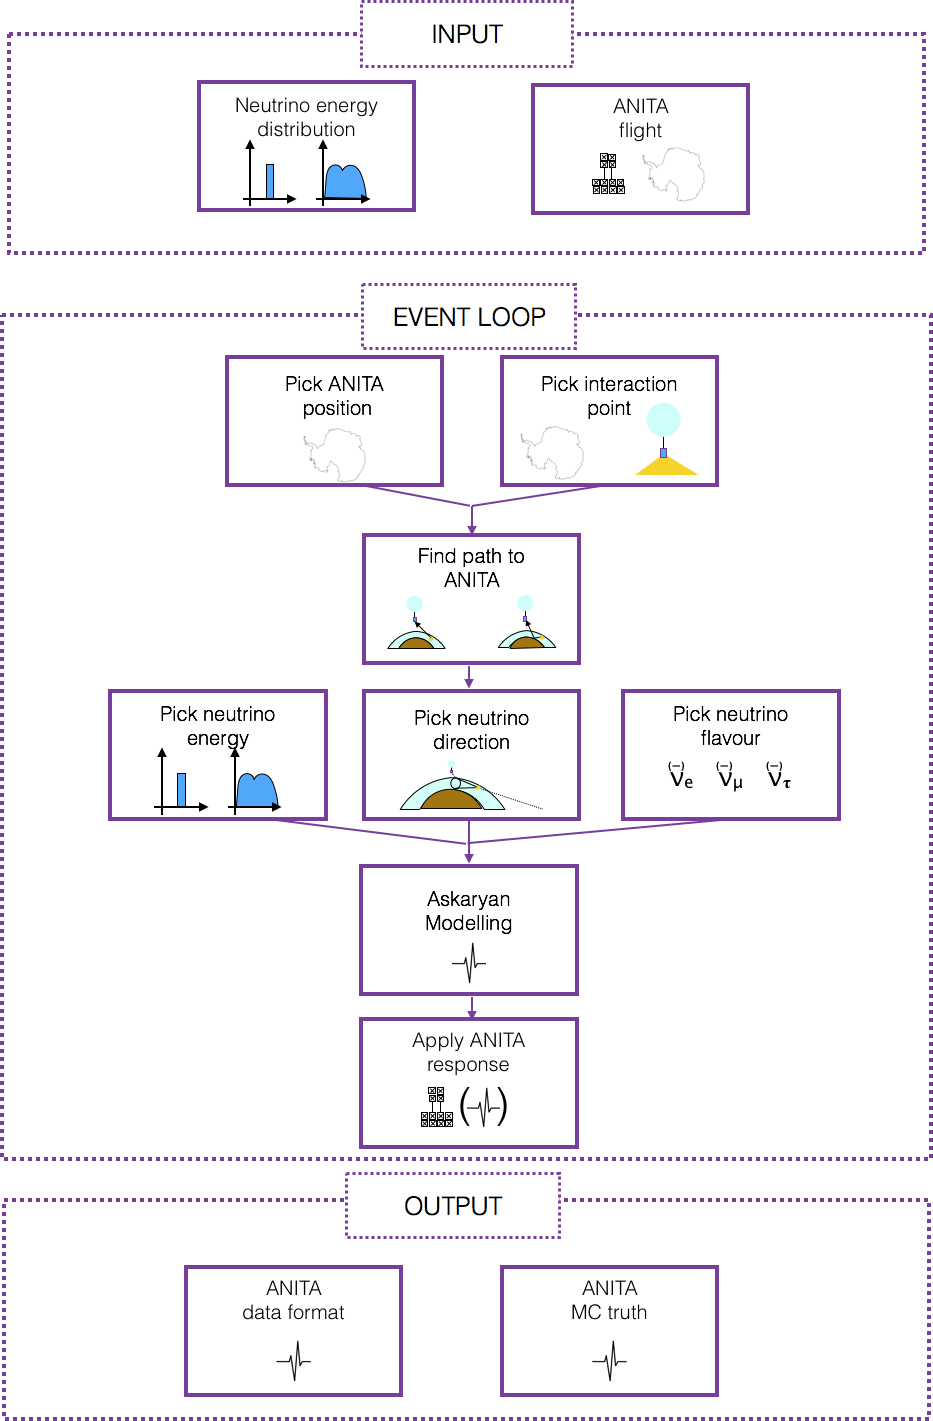
\includegraphics[width=.8\linewidth]{./Figs/IcemcFlowchart.png}
  \caption{Flowchart of the \icemc simulation for a single candidate.}
  \label{fig:intro_icemcFlow}
\end{figure}

A flowchart of the \icemc simulation steps is shown in Figure~\ref{fig:intro_icemcFlow}.
At the beginning of each run the user can choose which ANITA flight to simulate and which neutrino energy spectrum to use.
For each neutrino event, the position of the payload along the ANITA flight path, as well as the neutrino interaction position are randomly chosen.
These are used to find the path to the ANITA detector (Section~\ref{sec:eventGeometry}). 
The neutrino direction is then chosen within detectable angles; the neutrino energy is chosen following the input theoretical model; and the neutrino flavour and interaction type are chosen according to their expected ratios. 
These parameters are used to produce the radio-frequency pulse following the Askaryan model described in Section~\ref{sec:rf}.
The signal is then propagated through the ice and air to the ANITA
detector (see Section~\ref{sec:propagation}). 
The response of the ANITA signal chain is simulated, and the resulting 
data are saved in the same format as ANITA flight data 
(see Section~\ref{sec:ANITA}).
Different parts of the simulation are validated against data taken
both at the NASA Long Duration Balloon Facility
before the launch and in-flight during the past ANITA flights (see
Section~\ref{sec:validation}).
Finally the neutrino acceptance of the third and fourth ANITA flights, and
the contributions of the different parts of the simulation to the uncertainties on the acceptance are presented in Section~\ref{sec:results} .


\section{The ANITA flights}
\label{sec:anita3}
The first two ANITA payloads flew in 2006-2007\cite{ANITA1paper} and 2008-2009\cite{ANITA2paper,ANITA2erratum}, respectively.
Although \icemc can be used to simulate older flights, this paper focuses on the simulation of the third and fourth flights.

Figure~\ref{fig:ANITA_flightPath} shows the flight paths of the ANITA-III and ANITA-IV instruments. 
The color map shows the Antarctic ice depth. 
The third ANITA payload (ANITA-III) launched on December 18$^{\text{th}}$, 2014 from the
NASA Long Duration Balloon (LDB) facility near McMurdo Station, Antarctica.
ANITA-III followed the polar vortex flying at the altitude of 37\,km for
22 days until January 9$^{\text{th}}$, 2015 when the flight was terminated
near the Australian Davis Station.
Similarly, the fourth ANITA payload (ANITA-IV) launched on December 2$^{\text{nd}}$, 2016 from the NASA LDB facility in Antarctica and landed approximately 100\,km from the South Pole Station on December 29$^{\text{th}}$, 2016.


\begin{figure}[!h]\centering
  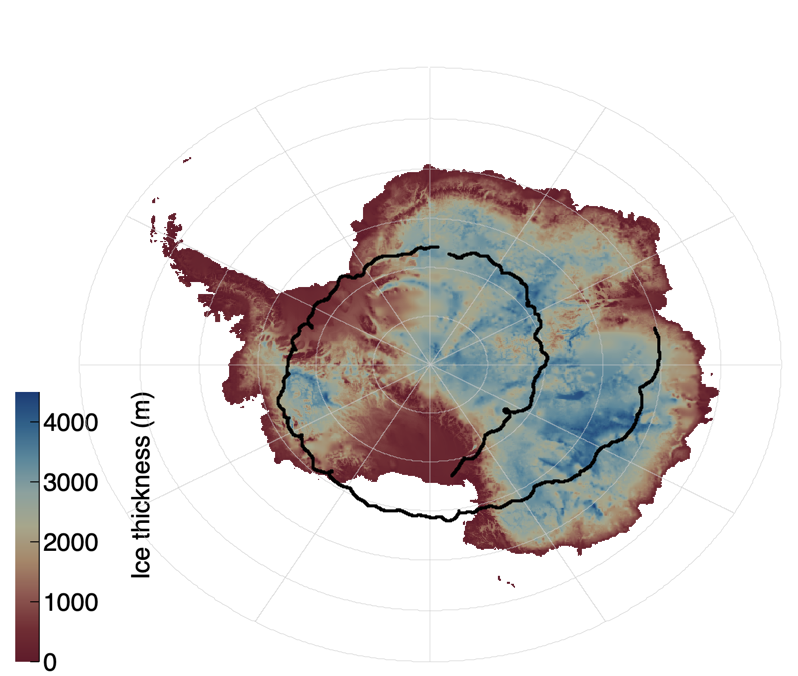
\includegraphics[width=.45\linewidth]{./Figs/Flightpath_ANITA3.png}
  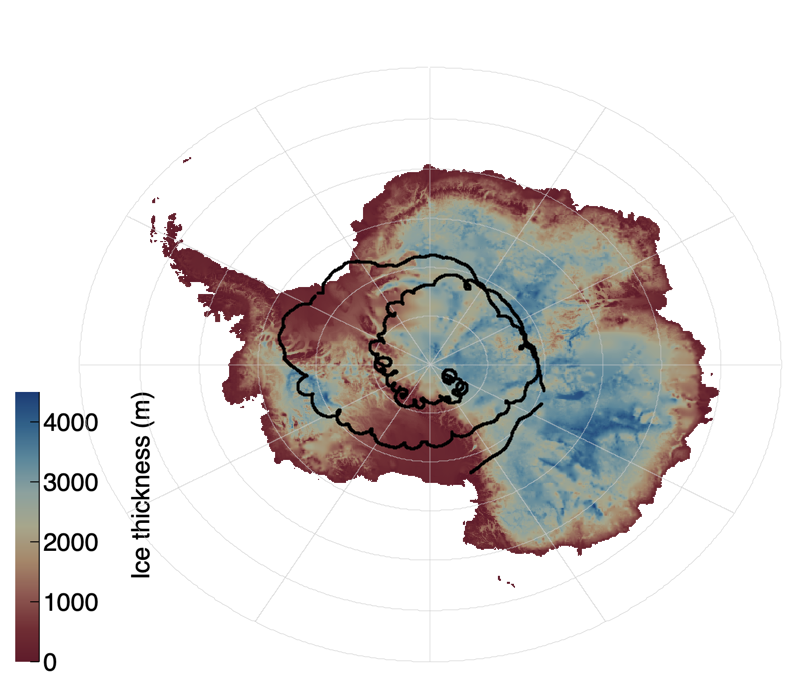
\includegraphics[width=.45\linewidth]{./Figs/Flightpath_ANITA4.png}
  \caption{Flight path simulated in \icemc for the ANITA-III (left) and ANITA-IV (right) flights.
    Antarctica map produced using the BEDMAP model~\cite{bedmap}.     }
  \label{fig:ANITA_flightPath}
\end{figure}



\begin{figure}[!h]\centering
  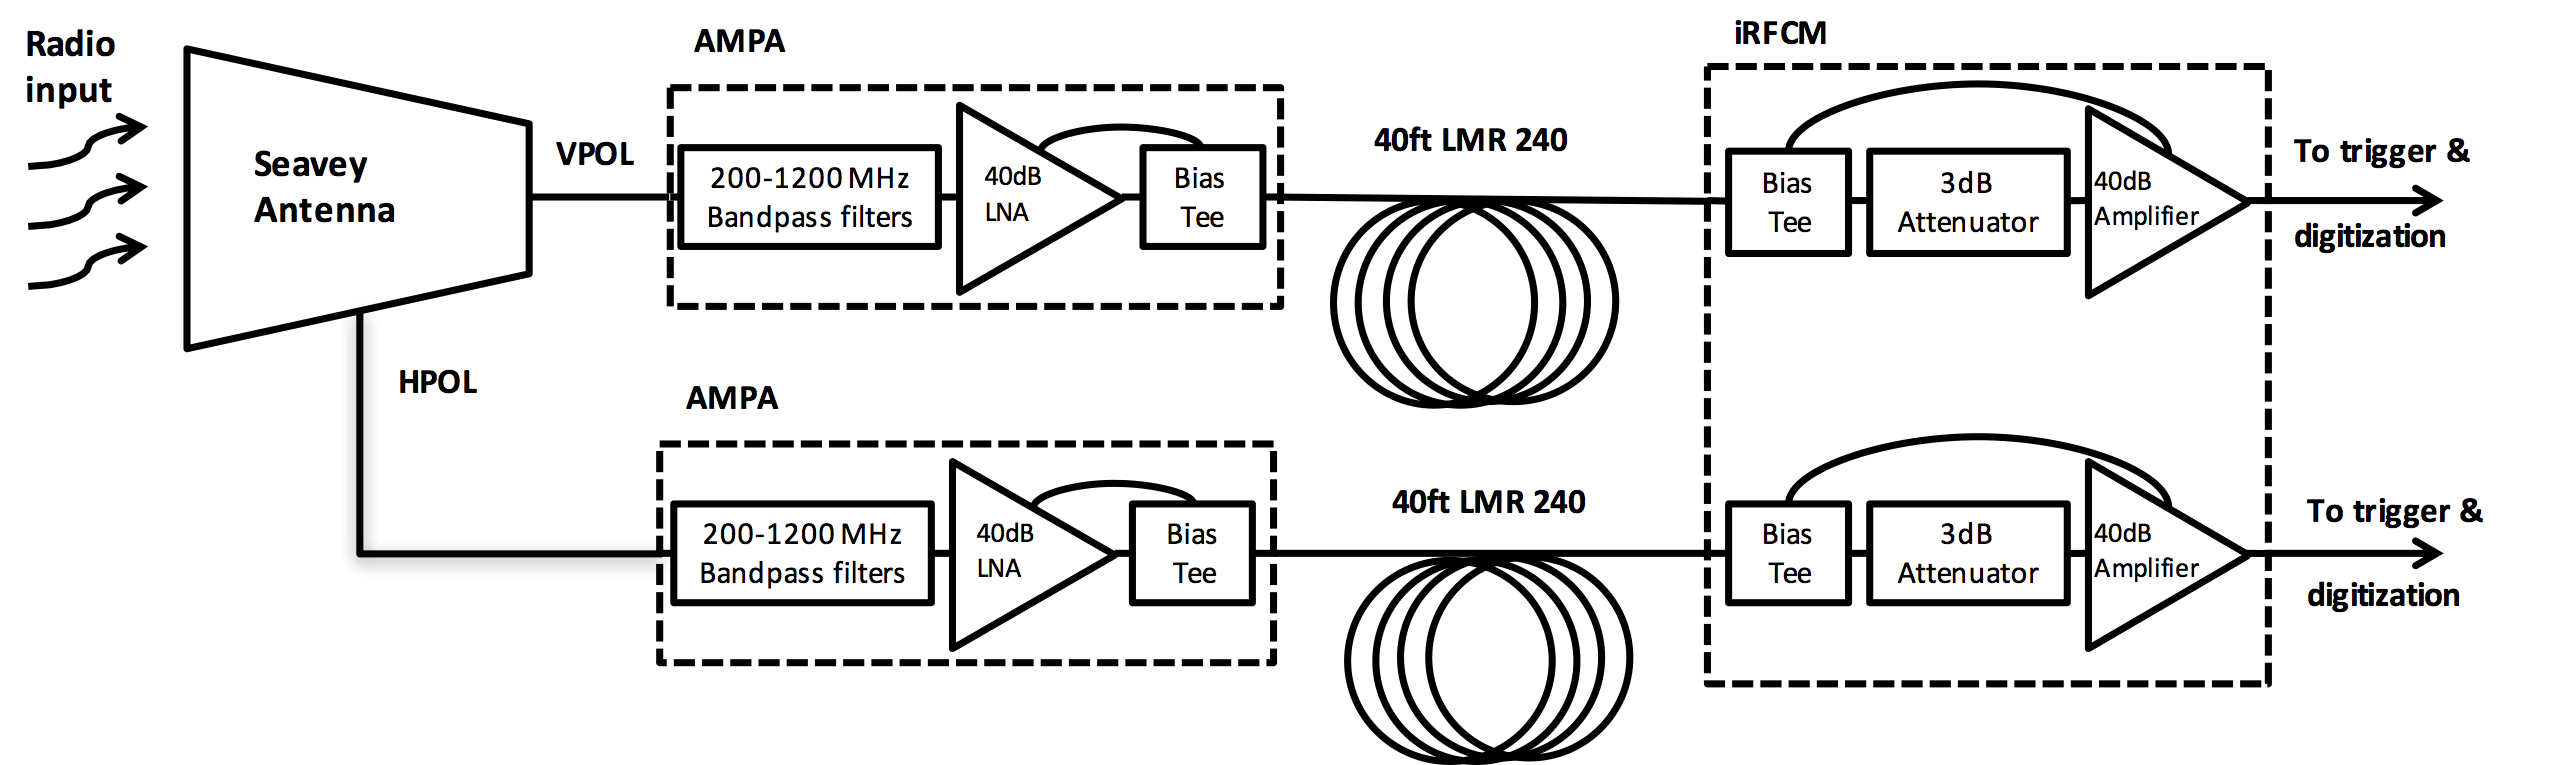
\includegraphics[width=.95\linewidth]{./Figs/ANITA3_signalChain1.png}
  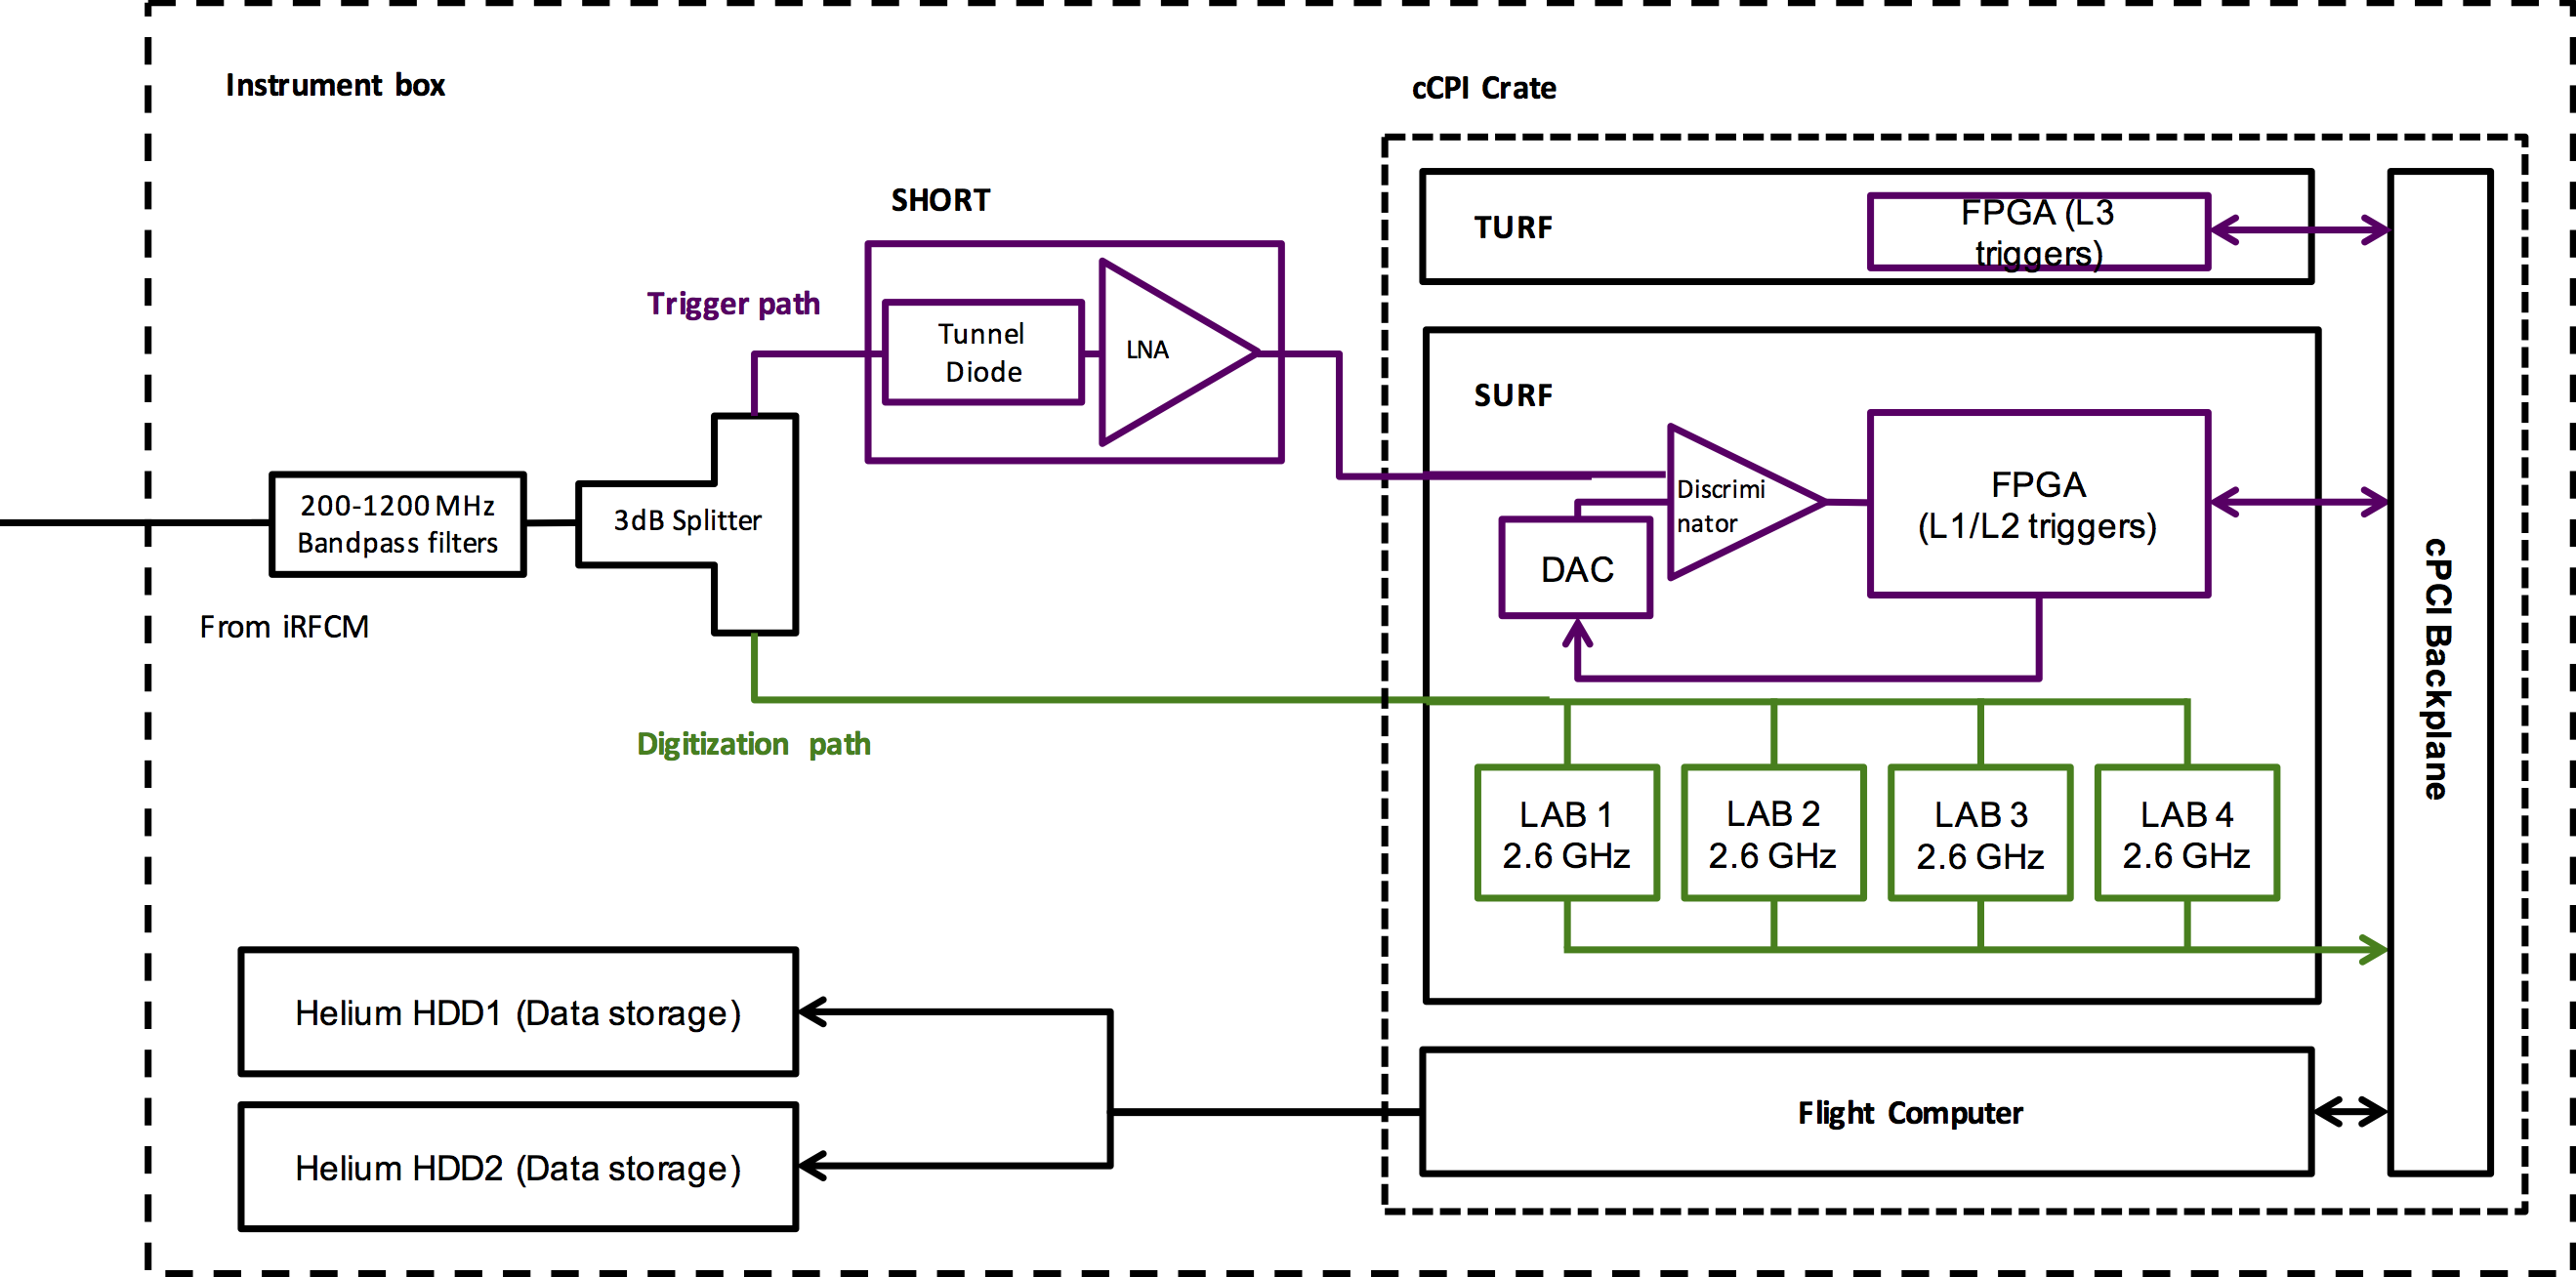
\includegraphics[width=.95\linewidth]{./Figs/ANITA3_signalChain2.png}
  \caption{ANITA-III signal chain.
  The receiving antenna splits signals into vertical and horizontal
  polarizations which follow identical paths. 
After going through filters and amplifiers, the signal is split into
the trigger and digitizer paths. In the trigger path the signal passes
through a tunnel diode and is compared to a threshold. 
When a trigger is issued, a switched capacitor array digitizes the
signal with a mean sample rate of 2.6\,GSa/s.}
  \label{fig:ANITA3_signalChain}
\end{figure}


The ANITA-III and ANITA-IV instruments were similar to the two previous
ones~\cite{ANITA1paper,ANITA2paper}, using 48 dual-polarization quad-ridged horn antennas with bandwidth from 200 to 1200\,MHz. 
The antennas were arranged in three rings forming 16 azimuthal sectors per ring, with the top ring divided into two layers to fit the launch envelope specifications, as shown in Figure~\ref{fig:intro_ANITAconcept}.

Figure~\ref{fig:ANITA3_signalChain} shows a schematic of the ANITA-III signal chain. 
The receiving antenna measures vertical and horizontal polarization components of incident radio waves, which then follow twin paths. 
After passing through filters and amplifiers, the signal is split into
the trigger and digitizer paths.
In the trigger path the signal passes
through a tunnel diode which acts as a square-law detector over the
input. The output of the tunnel diode is compared to the channel
threshold, which is dynamically adjusted by a PID loop to maintain the
rate for each antenna around 500\,kHz. A combination of first-level (L1) and second-level (L2) triggers forms a
global trigger which can be issued in each polarization.
When a trigger is issued, a switched capacitor array digitizes the signal with a mean sample rate of 2.6\,GSa/s. 
The ANITA-IV signal chain included the Tunable Universal Filter Frontend boards (see Subsection~\ref{subsec:tuffs}), and $90^{\circ}$ hybrids to convert the signals into left- and right- circularly polarized (LCP and RCP) components. 
The ANITA-IV trigger logic also required a coincidence between LCP and RCP signals within a 4\,ns coincidence window to select for linearly polarized signals. 

As the payload rotates freely, two sets of GPS units were used
independently to determine the
payload position and attitude.
Power was supplied by an octagonal array of photovoltaic panels and stored using four pairs of 12-V lead-acid batteries.
Communication to and from the payload was through the Iridium and TDRSS satellite systems throughout the flight, and by a direct line-of-sight radio link when within range of McMurdo Station.






\section{Event Geometry}
\label{sec:eventGeometry}

\subsection{Modeling the Antarctic continent}
Crust 2.0~\cite{crust2} is used to model the Earth's interior near the 
surface.  It is based on seismological data published from the Cooperative Studies of the Earth's Deep Interior (CSEDI).
The model gives thicknesses and densities of seven material
layers in $2^{\circ} \times 2^{\circ}$ bins:  ice, water, soft sediments, hard sediments, upper crust,
middle crust, and lower crust.  
%The ice thicknesses in Crust 2.0 are 
%claimed to be within 250\,m of the true ice thickness. Sediment thicknesses 
%in each cell are to within 1.0\,km of the true sediment thickness 
%and crustal thickness are within 5\,km of the true crustal thicknesses. 

The total Antarctic ice volume is computed by summing the product of ice
thickness and surface area for each bin within the Antarctic continent.
The area of each bin is calculated following:
\begin{equation}
\int_{\phi_1}^{\phi_2}\int_{\theta_1}^{\theta_2}\sin{\theta}~d\theta~d\phi=\left(\phi_2-\phi_1\right)\times\left(\cos{\theta_1}-\cos{\theta_2}\right) \, ,
\end{equation}
\noindent where the limits of the integrals define the edges of the bin in
latitude and longitude.
The \icemc program finds $2.976 \times 10^{16}$ m$^3$ of Antarctic ice in this model, compared to $3.011 \times 10^{16}$ m$^3$ reported by the US Geological Survey~\cite{usgs} (1.15\% difference).

%It is also possible to run the simulation using BEDMAP ice thickness
%and subglacial topographic model of Antarctica, developed by the
%British Antarctic Survey~\cite{bedmap}
%This model has a much more accurate representation of the ice in
%Antarctica, but it is much slower to run, so by default we use
%Crust2.0.
%When using BEDMAP the total volume of ice in Antarctica is found to be 
%$2.47956e \times 10^{16}$\,m$^3$. 

\subsection{Picking Interaction Point and Direction}
\label{sec:pickneutrino}

For each neutrino event, the payload position is chosen at random from a set of positions along the ANITA flight path (see Figure~\ref{fig:ANITA_flightPath}).
To simulate only those neutrino interactions that might lead to a detectable signal, interaction positions are limited to occur within the horizon as seen by the payload, and neutrino directions are chosen from an annulus on the sky consistent with viewing angles detectable at the payload (see Section~\ref{sec:weights}).
%from the Cherenkov angle at the payload (see Section~\ref{sec:weights}).

%maximum angle that the ray may diverge from the center of the Cerenkov cone for the interaction to still be detectable,
%\icemc uses importance weights to account for the neutrino interaction position forced to occur within the payload horizon, and for the neutrino direction chosen to allow the ANITA instrument to detect it (see Section~\ref{sec:weights}).

%Within that horizon, we stack the ice thicknesses of all the bins in longitude and latitude.  
%The height of each bin in the stack is the difference between the ice surface  and soft sediment elevations for that bin, which is the ice thickness.
%We pick a random point along the height of the stack to 
%determine which bin the interaction occurs in, and at what elevation within that bin.  
%The exact position of the interaction in the longitudinal and
%latitudinal directions is chosen at random within the bin.  
Half of the events thrown are assumed to come from a direct detection,
i.e. the signal is propagated from the interaction position upwards to
the payload.
For the other half of the events, the signal is propagated downwards
towards to the ice-rock interface (approximated to a flat mirror)
where the signal is then reflected upwards towards the payload. 

The neutrino interaction direction is chosen at random in the
elevation ($\theta$) and azimuth ($\phi$) space.
The elevation angle is constrained to values that would allow the interaction to be detected by ANITA. 

%Neutrino directions are only generated such that $|\theta_{\nu,ice}-\theta_{c}|<\theta_{th}$ where $\theta_{\nu,ice}$ is the angle  between the neutrino  direction and the direction from the interaction point in the ice, $\vec{n}_{ray}$ to the payload. 
%For direct rays $\vec{n}_{ray}$ is the direction of from the interaction point to the payload position; for reflected rays it is the mirror vector from the mirror interaction point to the payload, which means here $\vec{n}_{ray}$ is downward.
%The Cherenkov angle is $\theta_{c}=\mathrm{cos}^{-1}(1/n)$, see Section~\ref{sec:propagation} for how the index of refraction $n$ is chosen.   
%The angle $\theta_{th}$ is the maximum angle that the ray may diverge from the center of the Cherenkov cone for the interaction to still be detectable, given the parameters of the event.


%\subsection{Finding Earth/Ice Entrance Points for the Neutrino}
%\label{sec:entrance}
% Finding the entrance point for the neutrino $\vec{r}_{in}$,
%given $\vec{p}_{\nu}$ and $\vec{x}_{int}$
%is a simple geometry
%problem.  Define:
%%if (pow(R_EARTH,2)-pow(p,2)*(1-pow(costheta,2))>
%\begin{equation}
%    a\equiv p\times \cos{\theta}+\sqrt{R_{e}^2-p^2\cdot \sin^2{\theta}}
%\end{equation}
%where $\theta$ is the angle between $\vec{p}_{\nu}$ and
%$\vec{x}_{int}$, $R_e$ is the radius of the Earth.
%Then, the entrance point for the neutrino is:
%\begin{equation}
%    \vec{r}_{in}=\vec{x}_{int}-a\times\vec{n}_{\nu}.
%\end{equation}
%The quantity inside the square root is negative for events where
%the interaction occurred above sea level and the neutrino is
%down-going.  These events are treated separately and the
%entrance point is found iteratively.  
%First, the elevation $h^{(0)}_{int}$
%is found at the latitude and longitude where the interaction
%occurred, and then $R_e$ in the above equation is replaced with
%$R_e+h^{(0)}_{int}$ and a first guess at an entrance point is found.  Then
%the elevation at that latitude and longitude, $h^{(1)}_{int}$, is found
%and $R_e$ is replaced with $R_e+h^{(1)}_{int}$.  After four iterations,
%all but a few percent of the events have converged with a difference
%between entrance points by successive iterations being less than
%the interaction length for that energy.


\subsection{Event weighting}
\label{sec:weights}
To minimize computation time,
each event is weighted according to the probability of the neutrino reaching the detector, as well as
the "phase space" reduction (defined below), such that only those topologies that give measurable signal are fully simulated. 
As a neutrino moves through the earth, it encounters varying
densities as it passes through layers of the earth's interior,
and thus differing interaction lengths. 
The neutrino survival probability is thus calculated from the along-track
water-equivalent amount of material traversed.
%The probability that a neutrino interacts in the rock is:
%\begin{equation}
%\label{eq:weight}
%w_{survival}=\prod_{j=0}^{n}{e^{-x_j/L_j}}=\prod_{j=0}^{n}{e^{-x_j \rho_j/\ell }}=e^{\frac{1}{\ell}\sum_{j=0}^{n}{x_j \rho_j}}
%\end{equation}
%where $n$ is the number of layers the neutrino traverses.  A ``layer''
%can be the crust, the mantle, or one seven layers defined in Crust 2.0.
%Then $x_j$ is the distance the neutrino travels through the 
%$j^{th}$ layer in meters, $\rho_j$ is the density of the $j^{th}$ layer,
%$L_j$ is the interaction length 
%of that layer in meters,
%and $\ell$ is the interaction length in kg/m$^2$.

%The total chord length in kg/m$^2$ is calculated as follows.  
%We first step in 50\,m steps
%along the neutrino's path as it enters the earth through the 
%crust,
%summing over $x_i \rho_i$ where $x_i$ is the length of the $i^{th}$ 
%step and $\rho_i$ is the density the layer that contains that step.
%We continue stepping until we 
%are too deep to be in the earth's crust based on Crust 2.0.
%At each point, the depth along the neutrino path is calculated
%relative to the height of sea level according to the geoid model.
%Next, the distance that the neutrino travels through the
%mantle is found through a simple geometrical calculation.
%The density of mantle is taken to be 3400 kg/m$^2$.  The
%product of the path in the mantle and the mantle density
%is added to the sum.
%Then, we step through the remaining neutrino path to the
%interaction position, finishing the summation.


%\subsection{Phase Space Factor}
%\label{subsec:weightPhasespace}

The phase space factor is the product of the neutrino interaction
position and neutrino direction weights.
The position weight arises when the neutrino interaction position is
chosen only within the payload horizon.
This is calculated as
the ratio of the volume of ice within the horizon for the $i^{th}$
event and the total volume of ice in Antarctica (ratio of the yellow to blue
volumes in Figure~\ref{fig:weights}).
%product of the phase space factor that arises when
%the neutrino interaction position ($w_{pos}$)
%and the neutrino direction ($w_{dir}$) are chosen.
%Therefore,  $w_{phase-space}=w_{pos}\cdot w_{dir}$.
%The position of the neutrino interaction is forced to 
%be in the volume of ice that is 
%within the horizon of the balloon.
%The phase space factor $w_{pos}$ is then just the
%total volume of ice in Antarctica divided by the
%volume of ice within the horizon for the $i^{th}$ event.
%The volume of ice within the horizon is calculated once at the
%start of the program for 100 equally
%spaced balloon positions along its circular path.  For each event,
%we take the pre-calculated volume for the 
%balloon position that is closest to the balloon position for that event.
The neutrino direction is chosen such that its Cherenkov cone
lies close in solid angle to the direction from the interaction point to the payload. 
The correspondent weight is calculated as the ratio of the solid angle coming from the Cherenkov cone and a unit sphere (see purple cone in Figure~\ref{fig:weights}).

%it is possible that the event is observable 
%under the most optimistic of
%circumstances, as described in Section~\ref{sec:pickneutrino}.
%Since the direction for the $i^{th}$ neutrino is chosen from the intersection
%of a cone of width $2\sin{\theta_{th}}_i$ and a unit sphere, the corresponding phase space factor is:
%\begin{equation}
%w_{dir} =\frac{4\pi}{ \sin{\theta_{c}} \cdot 2  \sin{\theta_{th}} \cdot 2\pi}
%\end{equation}


\begin{figure}[!h]\centering
  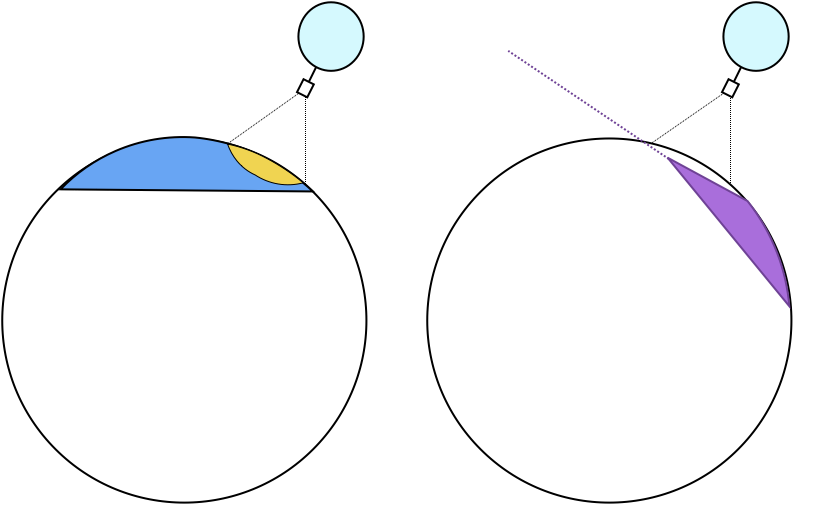
\includegraphics[width=.8\linewidth, trim = 0 6.5cm 0 0, clip]{./Figs/icemcWeightScheme.png}
  \caption{A schematic of the importance weights used in \icemc. The
    position weight arises because only interaction positions within
    the balloon horizon are simulated (yellow over blue area).
  The direction weight arises because only favourable directions within the
  Cherenkov cone are simulated (purple angle over a unit sphere).}
  \label{fig:weights}
\end{figure}


\section{Radio signal simulation} 
\label{sec:rf}

\subsection{Askaryan parametrization}
For each event the neutrino energy is picked randomly following the input energy spectrum.
Rather than simulating the particle shower development in the ice that
would produce the Askaryan radiation, a 1D parametrization is used 
to get the peak of the Askaryan signal at 1\,m from the point of interaction, $\mathcal{E}^{(\mathrm{@ 1m})}$, 
according to Reference~\cite{JaimeAskarian2000} and following:
\begin{equation}
\label{eq:vmmhz}
\mathcal{E}^{(\mathrm{@ 1m})} =2.53\times 10^{-7}\cdot \frac{\sin{\theta_{\mathrm{view}}}}{\sin{\theta_{\mathrm{Ch}}}}\cdot  \frac{E}{\mathrm{TeV}} \cdot \frac{\nu}{\nu_0} \cdot \frac{1}{1+\left( \frac{\nu}{\nu_0} \right)^{1.44}} \;,
\end{equation}
\noindent where $\nu$ is the frequency, $\nu_0=1.15$\,GHz, $E$ is
the shower energy (see Subsection~\ref{subsec:emhadshower}),
$\theta_{\mathrm{view}}$ is the viewing angle and $\theta_{\mathrm{Ch}}$ is the Cherenkov angle.
This parametrization is valid up to 5\,GHz, covering the ANITA
band of 0.2-1.2\,GHz.

\subsection{Neutrino flavors and interaction types}
\label{subsec:emhadshower}
The \icemc program assumes flavor democracy, assuming 
the flavors are fully mixed before the neutrinos get to the ice.
Information about each flavor is stored separately so the sensitivity to each flavor may be quoted separately.

The neutrino event undergoes a charged/neutral current interaction in
$69\%$/32\% of cases.
For charged current electron neutrino interactions, the electromagnetic
component is calculated as $1-y$, where $y$ is the inelasticity and is
approximated by a double-exponential function~\cite{gandhi}. 
In all other cases the electromagnetic component is considered negligible.
The hadronic component is equal to the inelasticity.
Secondary particles are not propagated.

\subsection{Cherenkov Cone}
\label{subsec:cherenkov_width}
The width of the Cherenkov cone is parametrized separately for the electromagnetic and hadronic components of the shower, according to References \cite{JaimeAskarian2000} and \cite{jaime05}, respectively.
The width of the electromagnetic
component in degrees is characterized by:
\begin{equation}
\label{eq:deltheta_em}
\Delta\theta_{em}(\nu)=2.7^{\circ} \cdot \frac{\nu_0}{\nu}\cdot \left(
  \frac{E_{LPM}}{ 0.14 E_{EM}+E_{LPM}} \right)^{0.3} \;,
\end{equation}
where 
$E_{EM}$ is the part of the shower energy associated with electromagnetic particles, and 
$E_{LPM}$ is energy above which the Landau-Pomeranchuk-Migdal
(LPM) effect becomes important.  
The LPM effect causes
the bremsstrahlung interaction to become suppressed because
the momentum transfer ($\propto k/E^2$) becomes so small 
that the Heisenberg uncertainty
causes the interaction to occur over many
scattering centers, resulting in destructive interference.  
This effect reduces the width of the Cherenkov cone, but not the magnitude of the electric field at the Cherenkov angle.
Following the recommendation in Reference~\cite{JaimeAskarian2000}, 
$E_{LPM}$ is set to $2\times10^{15}\ev$
and can be scaled to other media using the ratio of the respective radiation lengths.

The width of the Cherenkov cone for hadronic showers is modeled as laid out in Equation 9
in~\cite{jaime05}:
\begin{equation}
\Delta \theta_{\mathrm{had}} (\nu) =\frac{c}{\nu} \cdot
	\frac{\rho}{\mathrm{K}_{\Delta} X_0} \cdot
	\frac{1}{n^2-1} \;,
\end{equation}
\noindent where
$c$ is the speed of light,
$\nu$ is the frequency considered, 
$\rho$ is the density of ice,
$\mathrm{K}_{\Delta}$ is a normalization constant determined by a
separate Monte Carlo simulation~\cite{jaime05},
$X_0$ is the radiation length, and
$n$ is the index of refraction.

The signal strength at viewing angle $\theta$ 
away from the Cherenkov angle $\theta_{\mathrm{Ch}}$ is also parametrized following
Equation\,13 in Reference\,~\cite{jaime05}:
\begin{equation}
\mathcal{E}(\theta)=\frac{\sin{\theta}}{\sin{\theta_{\mathrm{Ch}}}} \cdot
\mathcal{E}(\theta_{\mathrm{Ch}})\cdot \exp\left[-\left(
    \frac{\theta-\theta_{\mathrm{Ch}}}{\Delta\theta_{\mathrm{em,had}}} \right)^2
\right] \;.
\end{equation}






\section{Propagation in ice and air}
\label{sec:propagation}

% The following equation is used for the index of fraction $n_{firn}$ as a function of altitude $h_{int}$ (a negative number in the firn here in meters), 
%\begin{equation}
%%n(h_{int})=1.325+0.463251\times e^{-0.140157\times h_{int}}
%n_{firn}(h_{int})=a+b\cdot e^{c\cdot h_{int}} \;,
%\end{equation}
%\noindent where
%$a=1.33$,
%$b=0.46$, and
%$c=-0.14$\,m$^{-1}$.
%This equation is a fit to the data measured by the 
 % See figure~\ref{fig:nrice}.
%\begin{figure}
%\begin{center}
%\epsfig{figure=nrice.eps,height=4.5in}
%\caption{Fit to RICE data for index of refraction as a function of depth below the surface.  Plot is from Peter Gorham.
%\label{fig:nrice}}
%\end{center}
%\end{figure}

%The specular paths through the ice and air are found through an iterative method.
%The initial seed for the surface RF exit point is the point on the ice surface directly above the interaction point.
%%From simple geometry we can calculate the surface normal, and smear it according to a Gaussian distribution of width 0.012 [WHERE DOES THIS COME FROM????] to account for surface ``slopeyness'' (this gives 0.01 rad as the mean magnitude of the slope).
%The second guess refines this by including Snell's law and the payload position.
%The in-air propagation vector, taken as the vector from the payload to the initial exit point seed, is refracted through the ice surface to determine its impact parameter with the interaction point (at constant depth).
%The exit point seed is shifted by this amount on the surface, and the refinement procedure is repeated.
%This allows for the calculation of the in-ice $\vec{n}_{ice}$ and -air $\vec{n}_{air}$ propagation vectors as well as the specular RF exit point $\vec{x}_{RF}$ on the ice surface.
%For reflected rays, we use the mirror interaction point instead. 
%A rejection cut is performed on the event based on the amount of expected attenuation,
%\begin{equation}
%F_{attn}(d_{ice}) = \mathrm{exp}(-d_{ice}\ /\ \ell_{attn}),
%\end{equation}
%due to the path length $d_{ice}$ and attenuation length $\ell_{attn}$ in ice.

The electric field is propagated to the payload using a standard ray tracing algorithm.
The electric field magnitude at the payload position (before applying
the ANITA instrument response) is calculated as follows:
\begin{equation}
 \mathcal{E}_{\perp,||} = \mathcal{E}^{(\mathrm{@ 1m})}  
 \mathrm{e}^{(-d_{\mathrm{ice}}\ /\ \ell_{\mathrm{attn}})}
 \frac{t_{\perp,||}}{d_{\mathrm{ice}} + d_{\mathrm{air}}}
 \ F(\theta_{\mathrm{view}}-\theta_{\mathrm{Ch}}) \,.
\end{equation}
The first factor after $\mathcal{E}^{(\mathrm{@ 1m})}$ accounts for propagation in ice, with $d_{\mathrm{ice}}$ being the path length and $\ell_{\mathrm{attn}}$ the attenuation length in ice. 
The second factor accounts for the refraction from ice to air, using
the specular Fresnel coefficients, $t_{||}$ and $t_{\perp}$, for the parallel and perpendicular components of the normalized transmitted electric field vector at the ice-air interface with respect to the local surface normal.
The surface normal includes a Gaussian 1.2\% direction perturbation to account for surface slope effects.
Finally, $F(\theta_{\mathrm{view}}-\theta_{\mathrm{Ch}})$ is a geometrical attenuation factor of the field strength in air resulting from viewing the Cherenkov emission at an angle $\theta_{\mathrm{view}}$ different from the Cherenkov angle $\theta_{\mathrm{Ch}}$.
The functional form of $F$ is taken to be Gaussian and is set to zero for ($\theta_{\mathrm{view}}-\theta_{\mathrm{Ch}}$) > 20 $\Delta \theta_{\mathrm{Ch}}$, where $\Delta \theta_{\mathrm{Ch}}$ is the width of the Cherenkov cone. 
%The user may set the attenuation length for radio in ice to be  a constant value (conservatively 700\,m), 

Cherenkov radiation is radially polarized, and the in-ice polarization vector of the Cherenkov radiation is radially outward in the plane formed by
the neutrino velocity vector and the Cherenkov propagation vector.
Attenuation lengths for radio in Antarctica are based on measurements performed at the Ross Ice Shelf and the South Pole~\cite{smex}.
The index of refraction is taken as 1.79 for deep ice and 1.325 at the surface. A model for the firn, a layer of packed snow above the ice, based on data taken by the RICE Collaboration~\cite{PhysRevD.73.082002} is used at depths shallower than 150\,m.

Surface roughness acts to allow different portions of the ice surface to contribute transmitted power to the payload for a given event, because it allows new scattering geometries at the air-ice interface.
The University of Hawaii ANITA group developed a simulation program, used for the ANITA-I and ANITA-II flights, which included surface roughness effects. They found that ice surface roughness contributed to an increase in acceptance of roughly a factor of 50\% at low energy (close to $10^{18}$\,eV) and 40\% at higher energy.
\icemc currently does not include ice surface roughness effects, and hence provides a conservative estimate of the sensitivity of the ANITA flights. Future versions of \icemc will include these effects.

%\subsection{Fresnel Factor}

%When the rays from the Cherenkov cone reach the ice-air boundary they just obey boundary conditions and thus the magnitude of the electric field is altered and the signal traverses the boundary~\cite{dawn}.
%For the pokey case, the polarization vector is perpendicular to the plane of incidence, and for the slappy case the polarization vector is in the plane of incidence.  The general case is composed of both components.

%After dividing up the electric field emerging from the ice 
%into its ``pokey'' and
%``slappy'' components, $E^{ice}_{\parallel}$ and 
%$E^{ice}_{\perp}$, the
%electric field that emerges from the ice $E_{air}$ is
%\begin{equation}
%E_{air}=\sqrt{\left( E^{ice}_{\parallel}\cdot r_{\parallel} \right)^2 + \left( E^{ice}_{\perp} \cdot r_{\perp} \right)^2 }
%\end{equation}



%\subsection{Ice Surface Roughness}
%\label{subsec:roughness}
%Surface roughness acts to allow different portions of the ice surface to contribute transmitted power to the payload for a single event, due to new allowable scattering geometries at the air-ice interface.
%These geometries depend on the characteristics of the roughness at the interface.

%These contributions are estimated by gridding the surface in the vicinity of the specular RF exit point.
%Each point $i$ on the grid has individual local values for $\vec{x}_{RF}^{i}$, $\vec{n}_{air}^{i}$, and $\vec{n}_{ice}^{i}$.
%Using only the local surface normal $\hat{n}^{i}$, the local incidence $\theta_{inc}^{i}$ and transmission $\theta_{trans}^{i}$ angles are calculated; in other words, the ray tracing procedure for the specular case is not used in the geometry determination of grid point $i$, except to determine the placement of the grid using the RF exit point seed.

%A toy facet model was developed to determine the all-sky transmitted power distribution for specified roughness parameters.
%The simulation was validated with measurements of laser light refracting through ground glass diffuser plates~\cite{Griswold:07}; see Section~\ref{subsec:validation_lab} for additional information.
%Different Antarctic locations are characterized by different roughness parameters, for which this implementation is able to account.
%It is important to note that ($\theta_{inc}^{i}$, $\theta_{trans}^{i}$) pairs satisfy $local$ EM boundary conditions since the toy facet model generates a distribution of tilted surface facets allowing transmission.

%The simulation generates a distribution of tilted facet elements with slopes randomly sampled according to a Rayleigh distribution characterized by a rms slope value $s_{rms}$.
%For each element, the basic calculation involves projecting the incident ray along the facet element normal to determine the local incidence angle for use with Snell's law, as well as basis vectors oriented in the element plane.
%The local transmission vector is constructed from the element normal and basis vectors, then projected along the global surface normal to determine the direction relative to the global surface.
%This procedure is performed, for both parallel and perpendicular transmission, many times to provide the average transmitted intensity as a function of position on the sky.

%For a specified roughness parameterization, simulations of the facet model are used to generate look-up tables in ($\theta_{inc}^{i}$, $\theta_{trans}^{i}$), which are used by \icemc to estimate the contributed power for a given grid point $i$ and its associated geometry.
%Resources at the Ohio Supercomputer Center~\cite{OhioSupercomputerCenter1987} were used to perform the validations and generate high statistics look-up tables.
%The calculation for the transmitted electric field vector at the payload is otherwise the same as described above for the specular case, except that the specular Fresnel coefficients are replaced by ($Power^{1/2}$) for the respective field vector component.
%Since the total simulated time-domain waveform at the payload will be the sum of the individual waveforms, the relative time delay due to the varying path length\footnote{measured relative to the specular travel time} for each grid point is also recorded.





%%% Local Variables:
%%% mode: latex
%%% TeX-master: "icemc.tex"
%%% End:


\section{ANITA detector model}
\label{sec:ANITA}
The simulated signal is
propagated to the front of each of the ANITA antennas and through the
trigger and digitizer paths of the ANITA instrument, taking into
account the payload rotation.
The payload position chosen along the flight path is used to load appropriate information about the payload rotation, channel threshold values and channel masking.
The payload geometry is simulated using photogrammetry measurements
and phase-center calibration measurements taken with a ground pulser
during the flights.
Antenna gains measured in the lab previous to the flight are
applied to the signal according to the incident angles on the E and H planes. 

The signal then follows the signal chain as shown in
Figure~\ref{fig:ANITA3_signalChain}.
First, the incident fields are folded into the vertical-polarization (VPOL) and horizontal polarization (HPOL) responses of the antennas. 
The outputs of these components are divided into the trigger and digitizer paths.
The digitizer and trigger responses were measured before the flights
by injecting an RF signal directly into the amplifiers behind the
ANITA antennas and measuring the output of the digitizer and trigger paths. 
Figure~\ref{fig:ANITA_ImpulseResponses}~(left) shows the
power spectra of the trigger and digitizer impulse responses for a
sample channel of the ANITA-III payload.
To avoid continuous wave (CW) noise from satellite and station transmissions, ANITA-IV adopted 
tunable notch filters (see Section~\ref{subsec:tuffs} and Reference~\cite{Allison:2017vtk}).
Figure~\ref{fig:ANITA_ImpulseResponses}~(right) shows the
power spectra of the trigger and digitizer impulse responses for a
sample channel of the ANITA-IV payload with the most common filter configuration used during flight.
Thermal noise is generated based on flight measurements (see Section~\ref{subsec:ANITA_thermalNoise}) and added to the waveforms.
Finally, the modeled tunnel diode response (see
Section~\ref{subsec:ANITA_trigger}) is convolved with the signal
waveforms from all the channels, and if an event passes the trigger
logic, the RF signal and truth information about the neutrino
interaction are saved in the final output.

\begin{figure}[!h]\centering
  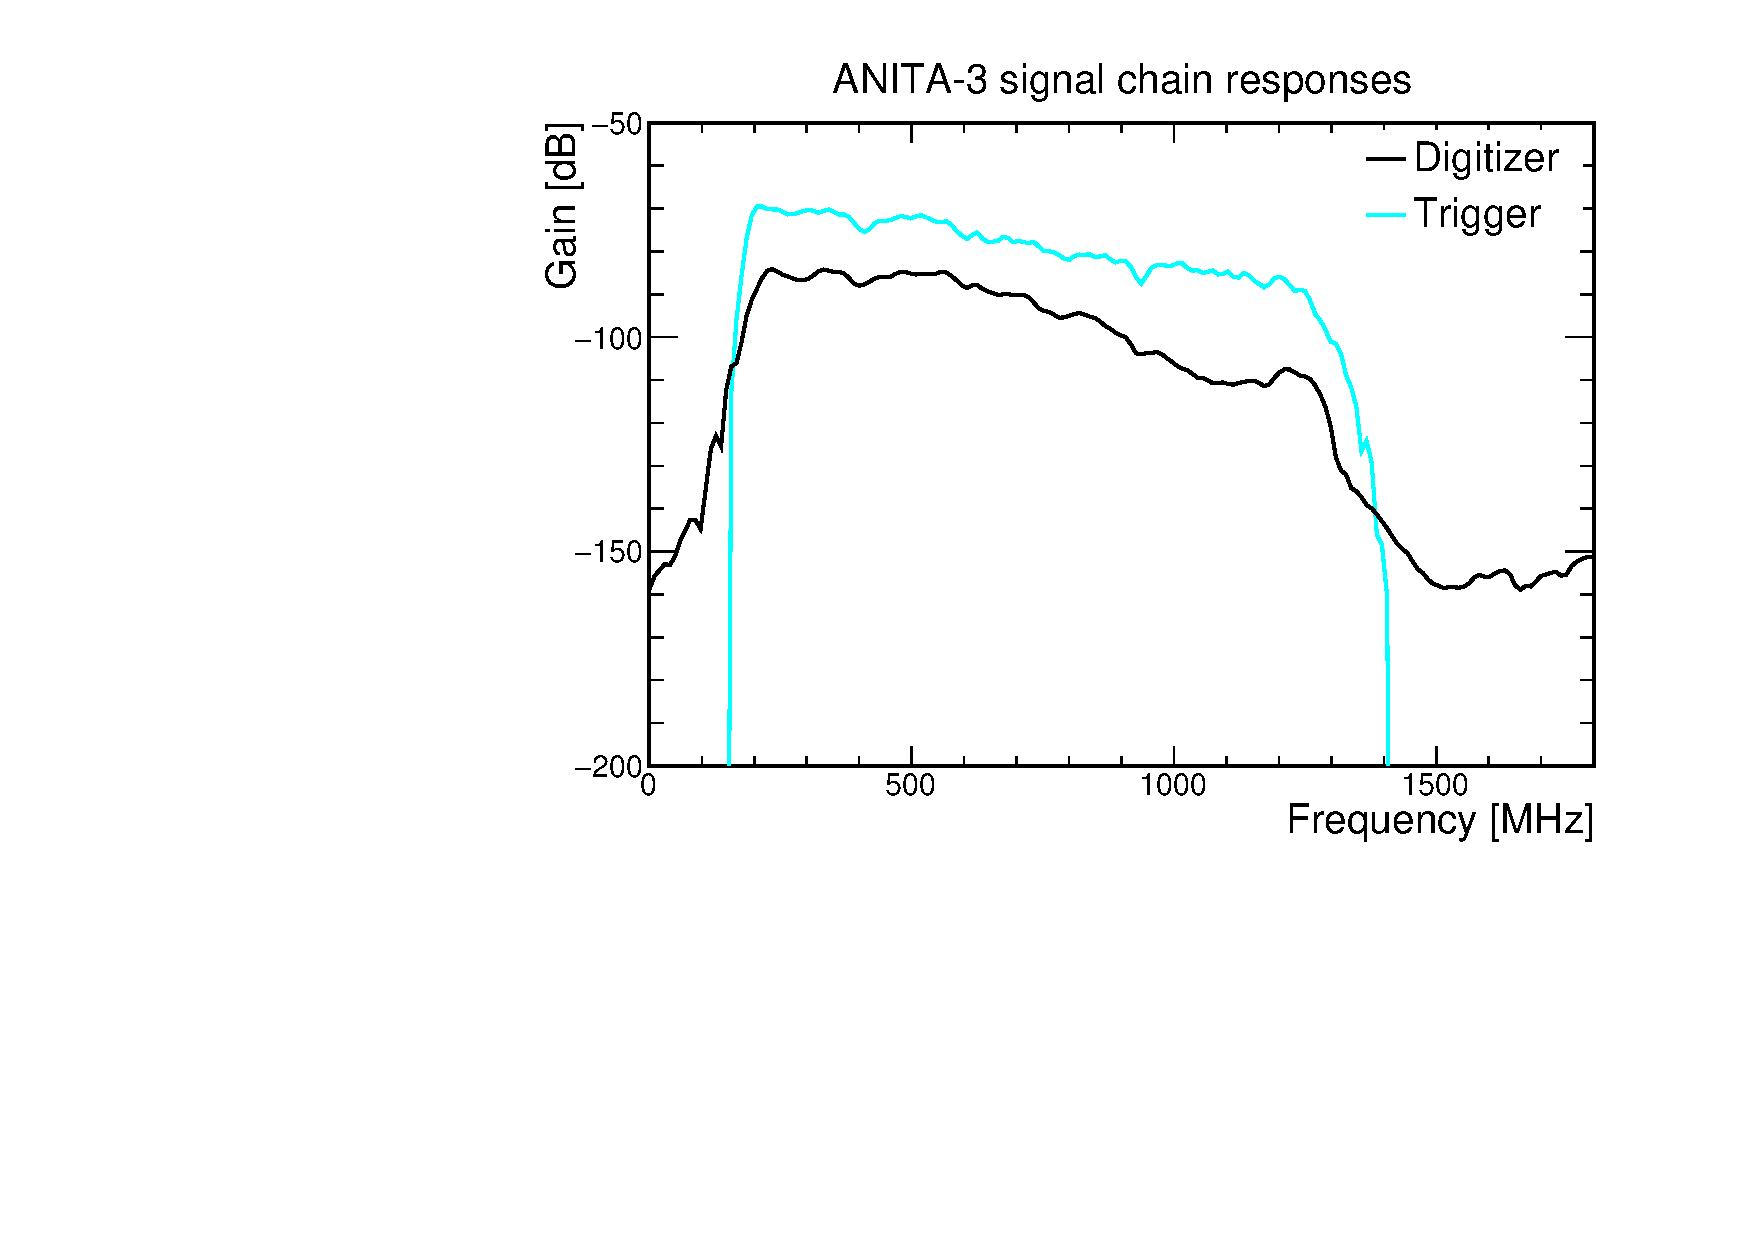
\includegraphics[width=.45\linewidth]{./Figs/A3ImpulseResponses.pdf}
  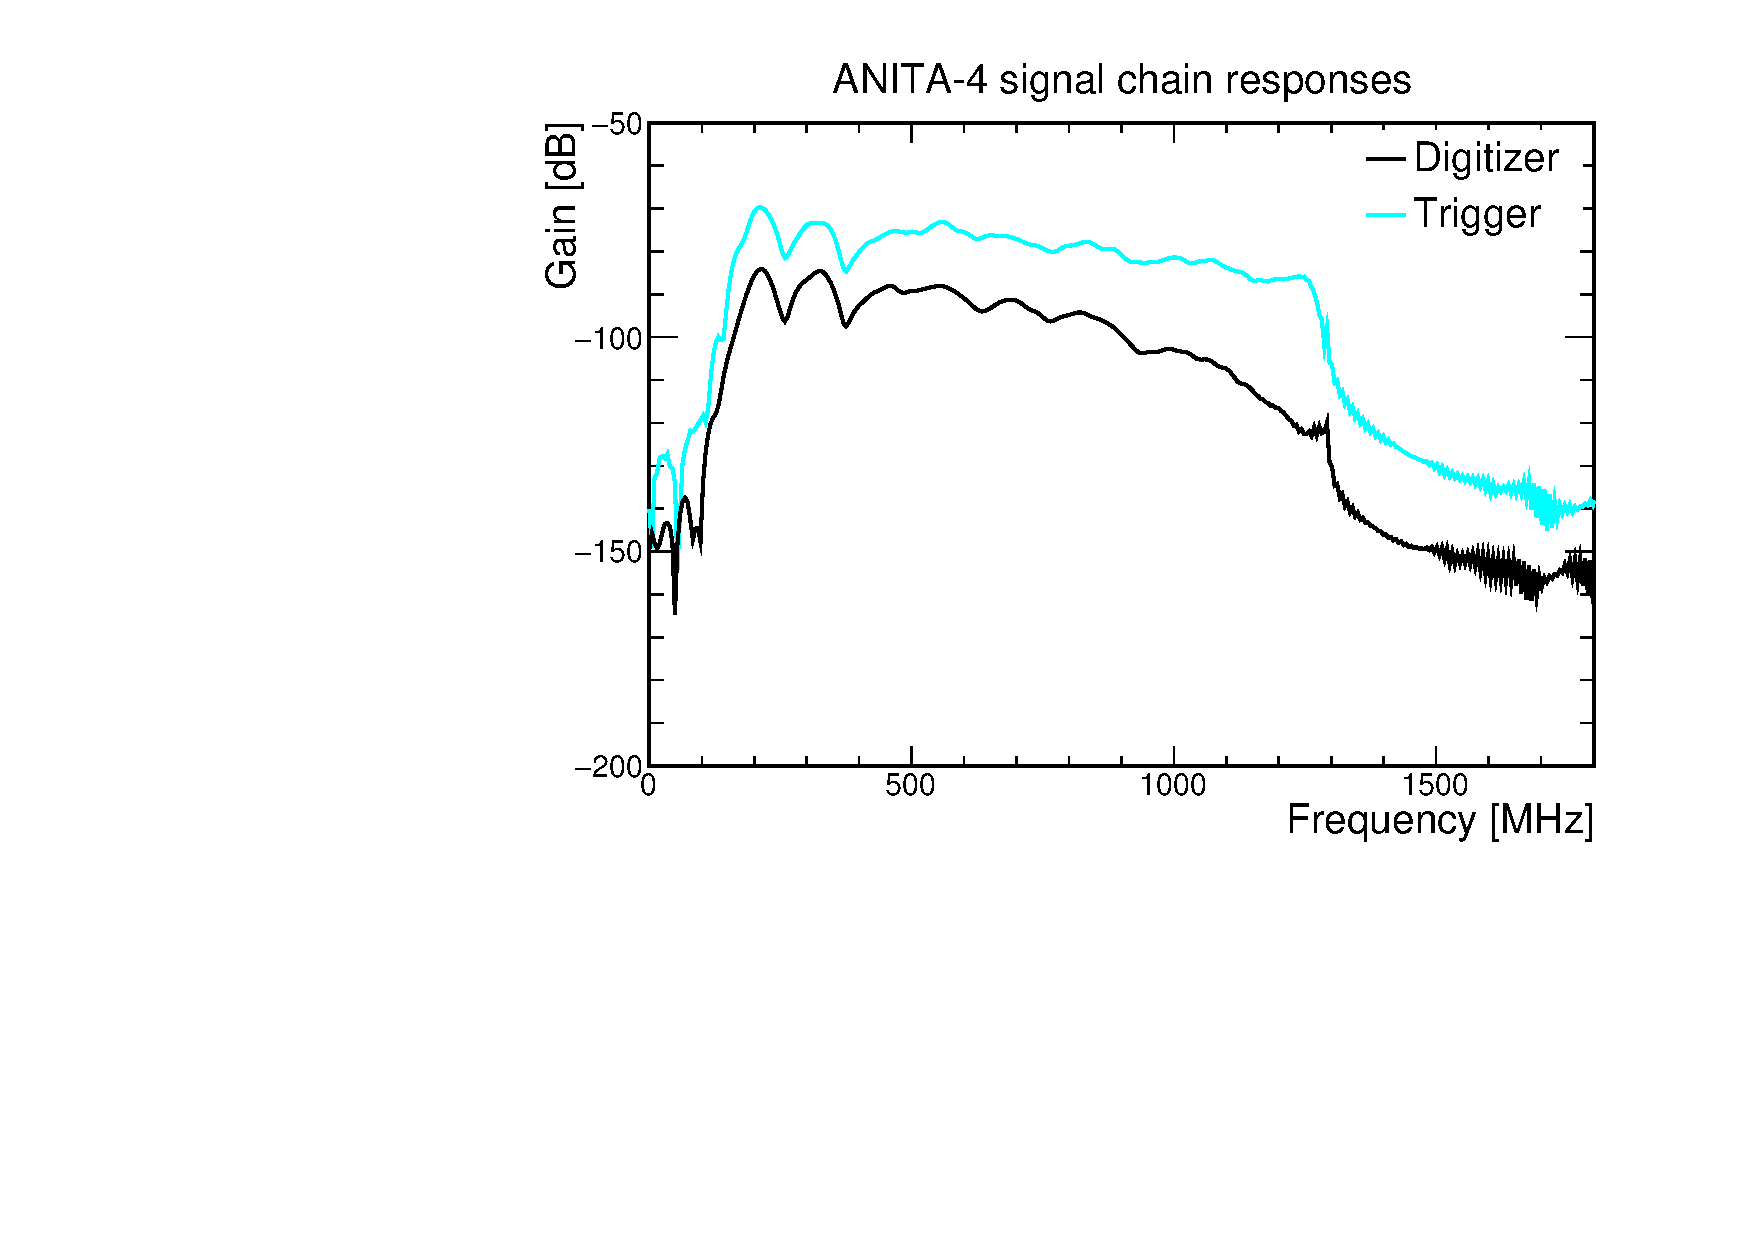
\includegraphics[width=.45\linewidth]{./Figs/A4ImpulseResponses.pdf}
  \caption{Power spectrum of the trigger and digitizer impulse
    response for a sample channel, for the ANITA-III (left) and ANITA-IV (right) instruments. 
    %\CD{Why is there power above Nyquist?}
    }
  \label{fig:ANITA_ImpulseResponses}
\end{figure}


\subsection{Tunable Universal Filter Front-end boards}
\label{subsec:tuffs}
To alleviate the anthropogenic noise observed in ANITA-III that caused
significant amounts of deadtime, ANITA-IV added the Tunable Universal
Filter Front-end, or TUFF, boards~\cite{Allison:2017vtk}.
This board uses up to three notches to attenuate
the gain by a maximum of 13\,dB around each notch
frequency:
the notches are tunable, but default to 260, 375, and 460\,MHz, corresponding to known satellite communications frequencies. 
Whether each notch is activated and at which frequency is called
a "configuration".
There were seven unique configurations for the ANITA-IV flight  which are simulated in 
\icemc. 
The measured TUFF response for the configuration when all notches are on and at default frequencies is plotted in Figure~\ref{fig:TUFFs}~(left). 
An example of the effect of the third notch switched on or off when 460\,MHz carrier wave noise is simulated is shown in Figure~\ref{fig:TUFFs}~(right).

The measured TUFF response for a given configuration is loaded
into \icemc and convolved with the trigger and digitizer impulse
responses for each channel. 

\begin{figure}
  \centering
 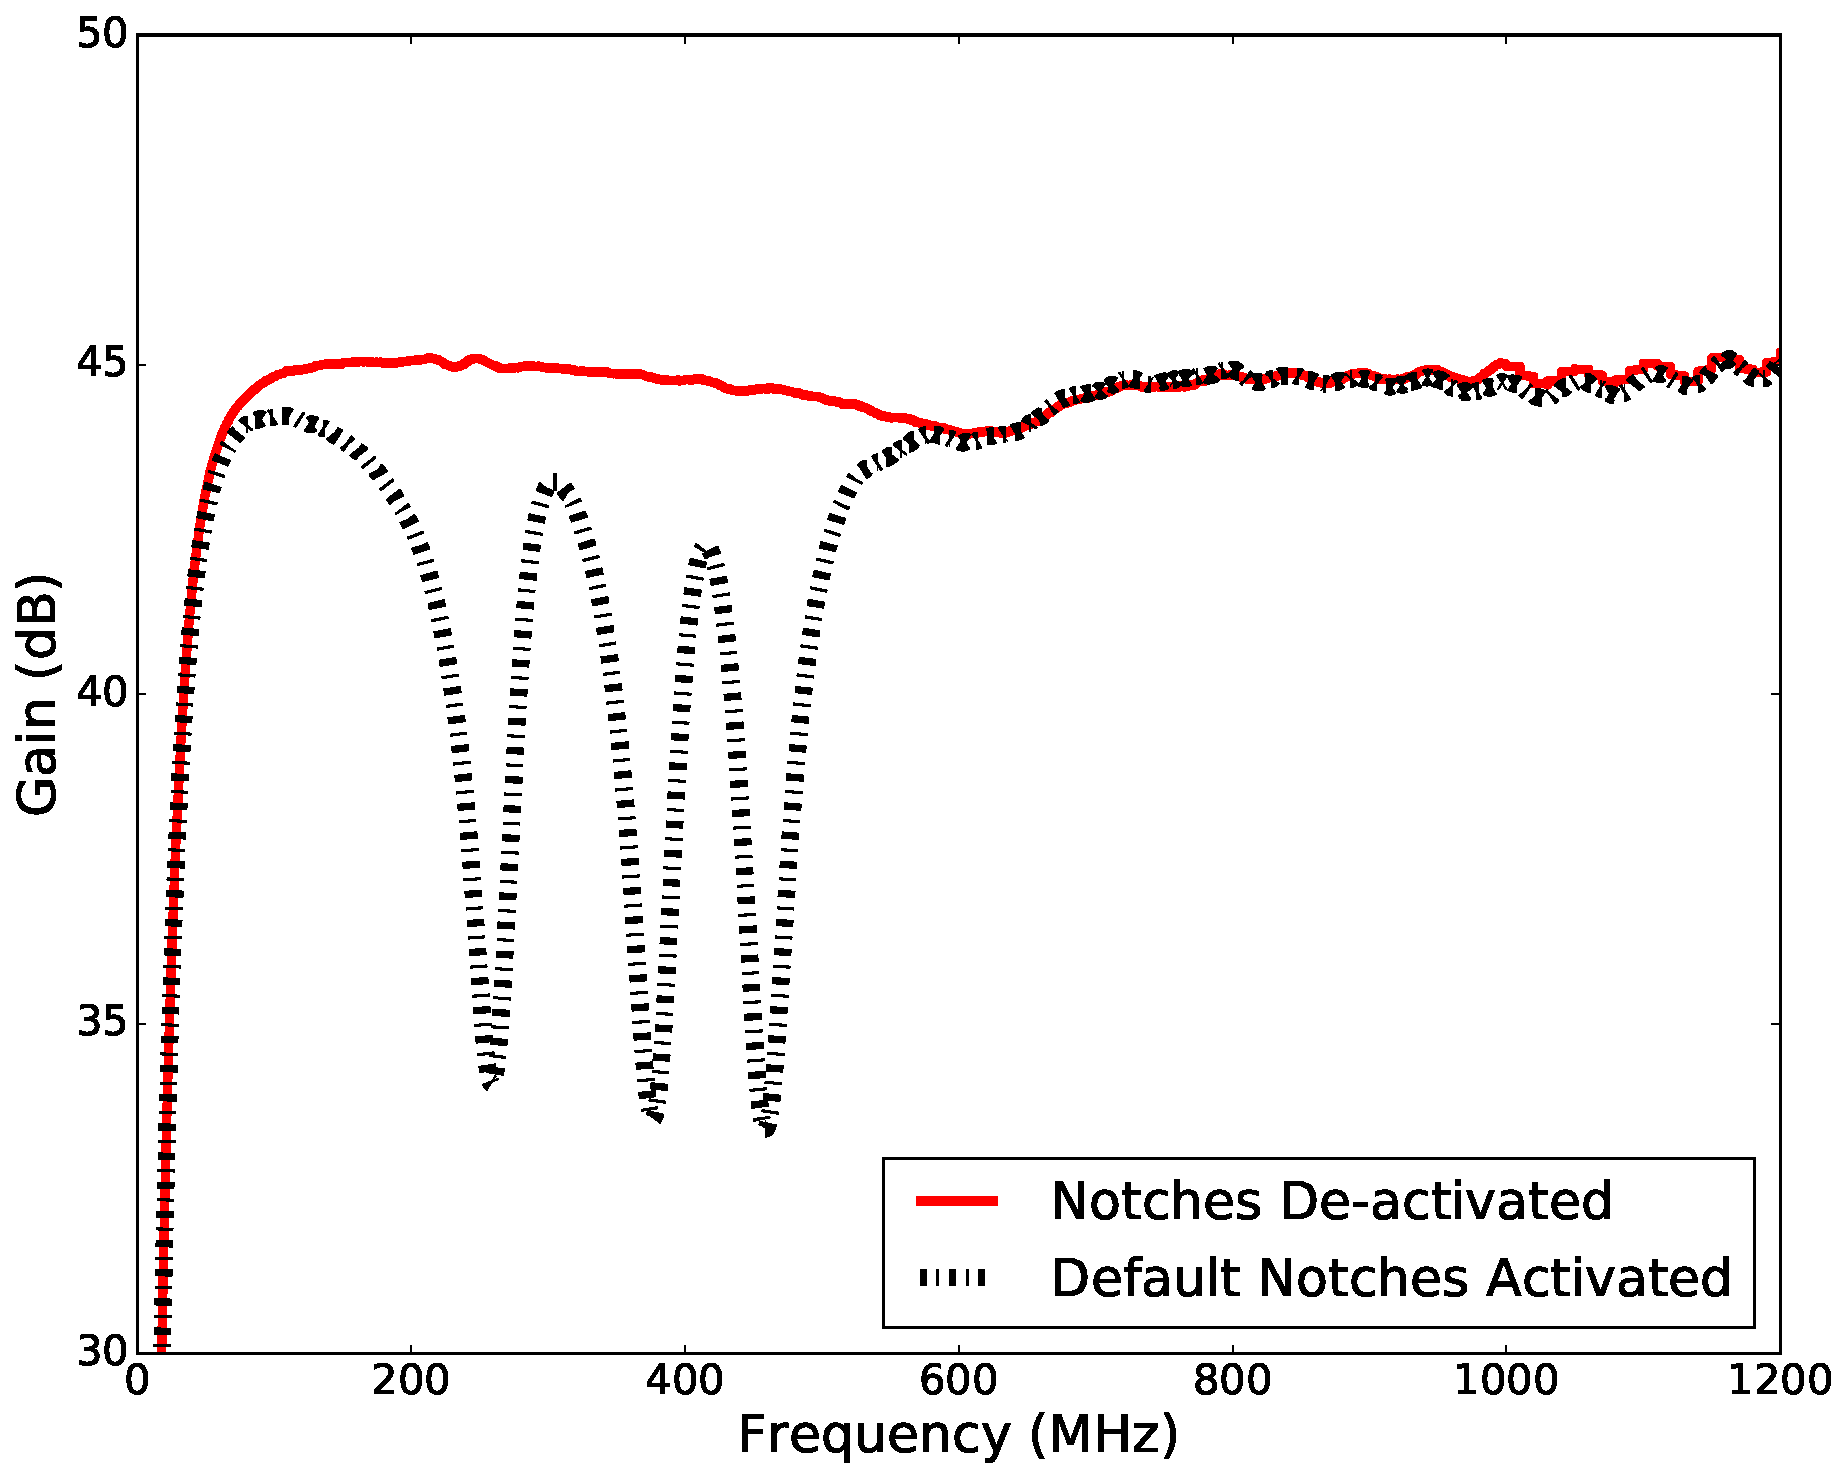
\includegraphics[width=0.4\linewidth] {./Figs/measured_gain_freq_on_off.pdf} 
 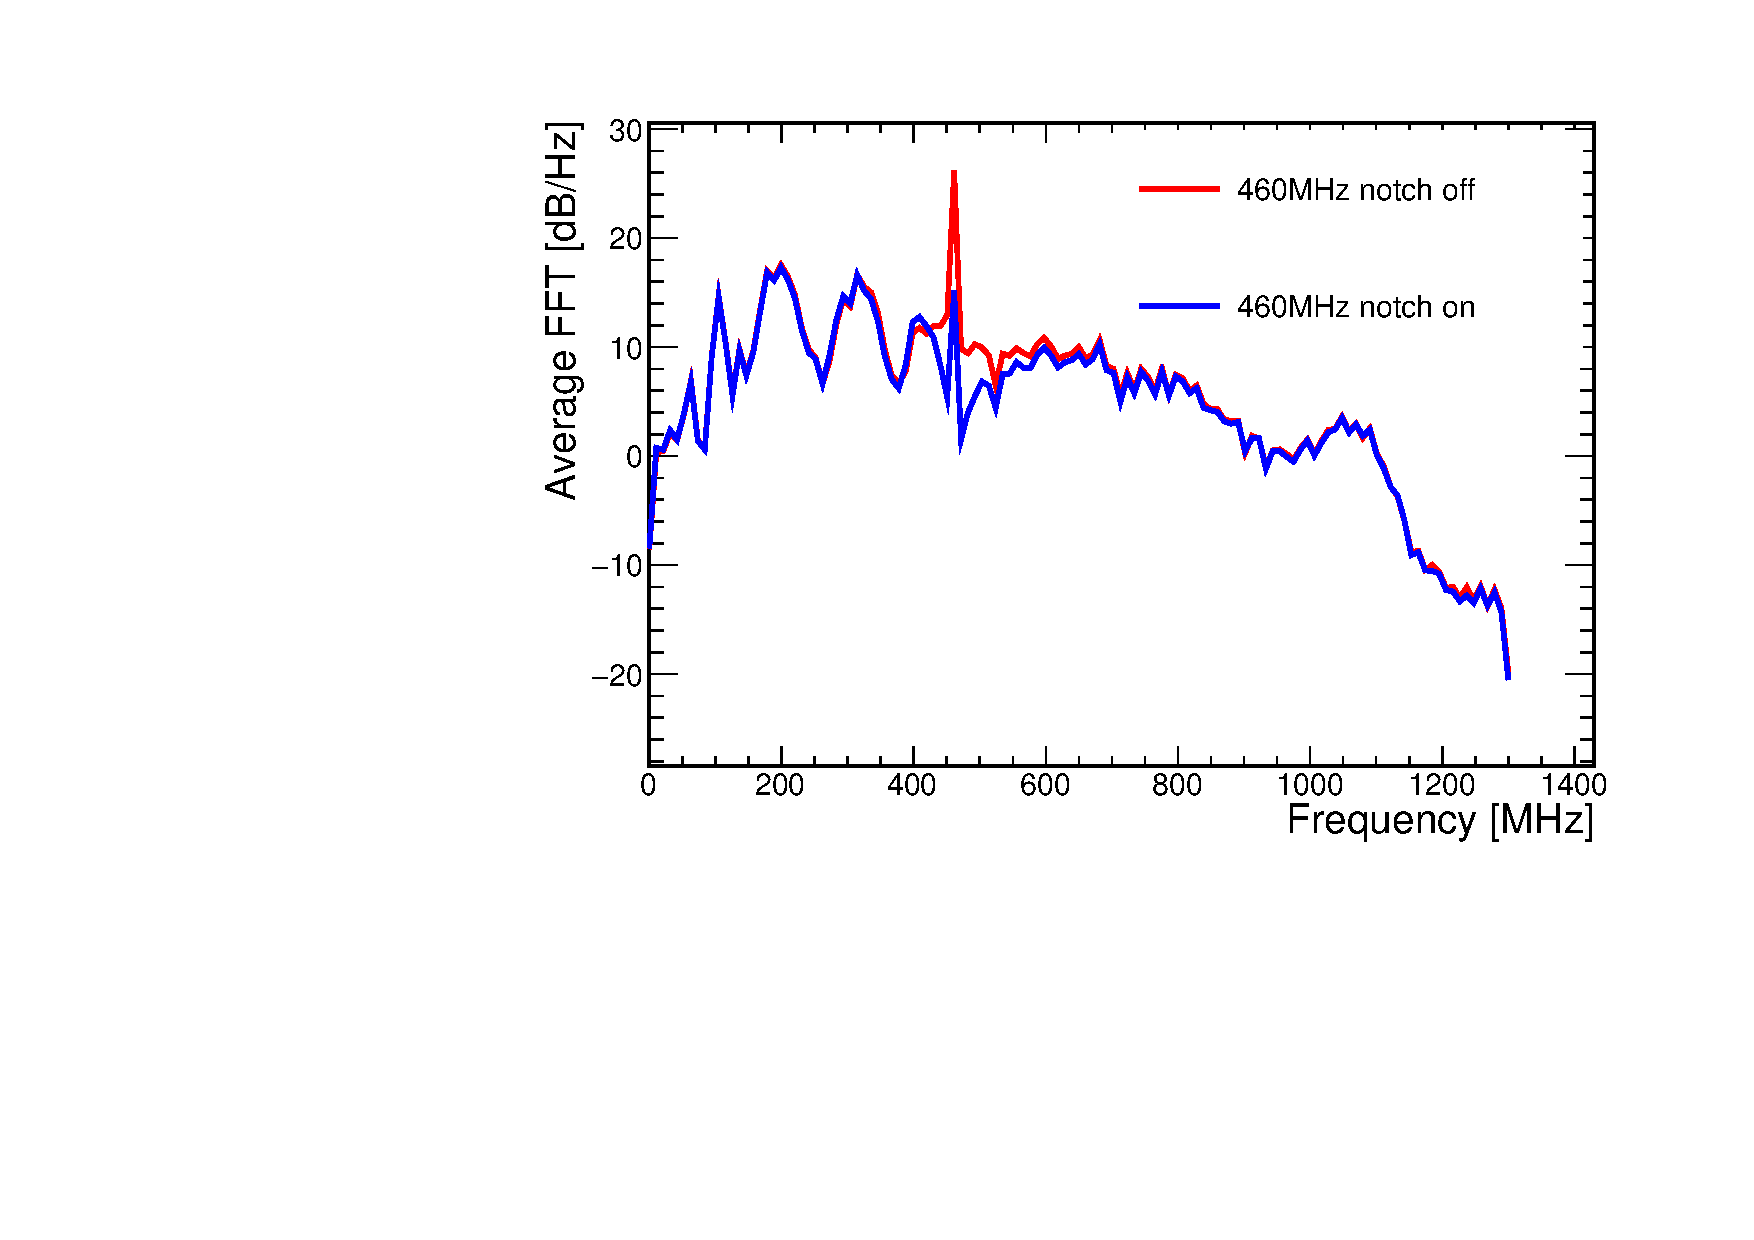
\includegraphics[width=0.45\linewidth] {./Figs/Icemc_tuffs.pdf} 
  \caption{(Left) Measured TUFF response in frequency domain (dB vs frequency) obtained in the lab. The dips in the response clearly mark the 260, 375, and 460 MHz notches turned on in this configuration and the 13\,dB attenuation at those frequencies is clear~\cite{Allison:2017vtk}.
  (Right) Example of carrier wave noise injected in \icemc with the third notch activated and not activated.}
\label{fig:TUFFs}
\end{figure}



\subsection{Thermal noise}
\label{subsec:ANITA_thermalNoise}
Modeling thermal noise correctly is crucial to the simulation of ANITA’s
sensitivity to neutrino interactions as it affects both the trigger and analysis efficiencies.
An accurate model of the thermal noise makes it possible to simulate both the
accidental noise triggers and the effect of noise fluctuations on the
reconstructed correlation maps used to calculate the event direction in the ANITA analyses~\cite{romero2015interferometric}.

To provide a realistic model of the thermal noise during the ANITA flights, events coming from minimum bias triggers during
a quiet time of the ANITA-III flight are used to produce power spectra in bins of 10\,MHz for each digitizer channel.
As the ANITA-III flight suffered more than the previous flights 
from continuous wave noise coming
from satellites and human bases, frequencies in the ranges
234-286\,MHz and 344-410\,MHz are filtered out in software analysis
using two simple notch filters. 
Data from antennas facing the sun were also excluded.

For each channel and each frequency bin a Rayleigh PDF is fit to the data:
\begin{equation} 
  f(A, \sigma)=\dfrac{A}{\sigma^2}e^{-A^2/(2\sigma^2)} \;,
  \label{eq:rayleigh}
\end{equation}
\noindent where $A$ is the amplitude in the frequency domain (in mV/MHz) and $\sigma$ is the
Rayleigh amplitude in that frequency bin.
As most of the carrier wave noise is in the tail of these
distributions, the Rayleigh fits are performed only to the rising edge and peak of the distributions.
Figure~\ref{fig:rayleighFits}(left) shows an example of Rayleigh distribution fits for a sample channel in the frequency bin centred at 710.94\,MHz.
Events in this sample come from minimum bias triggers during the ANITA-III quiet time.
 
\begin{figure}[!h]\centering
  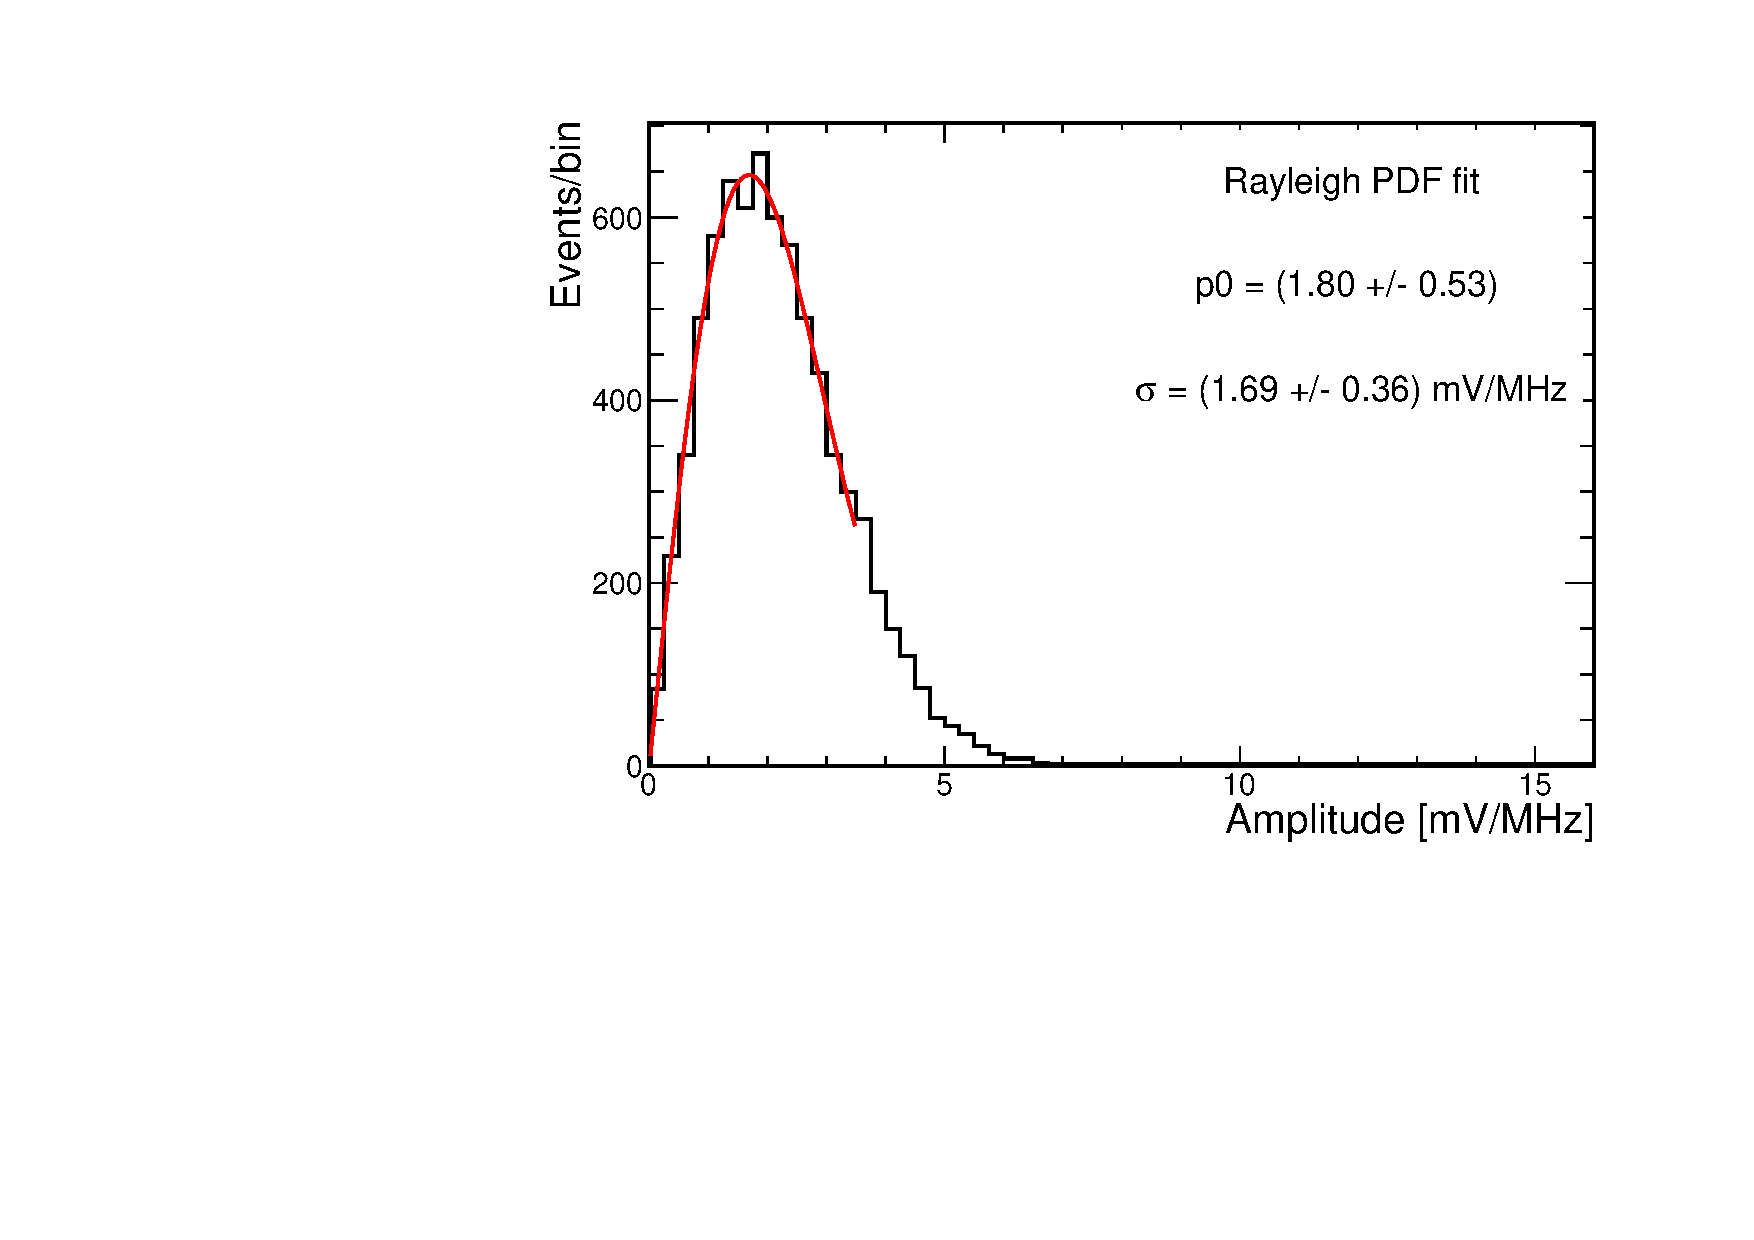
\includegraphics[width=.45\linewidth]{./Figs/RayleighExample.pdf}
  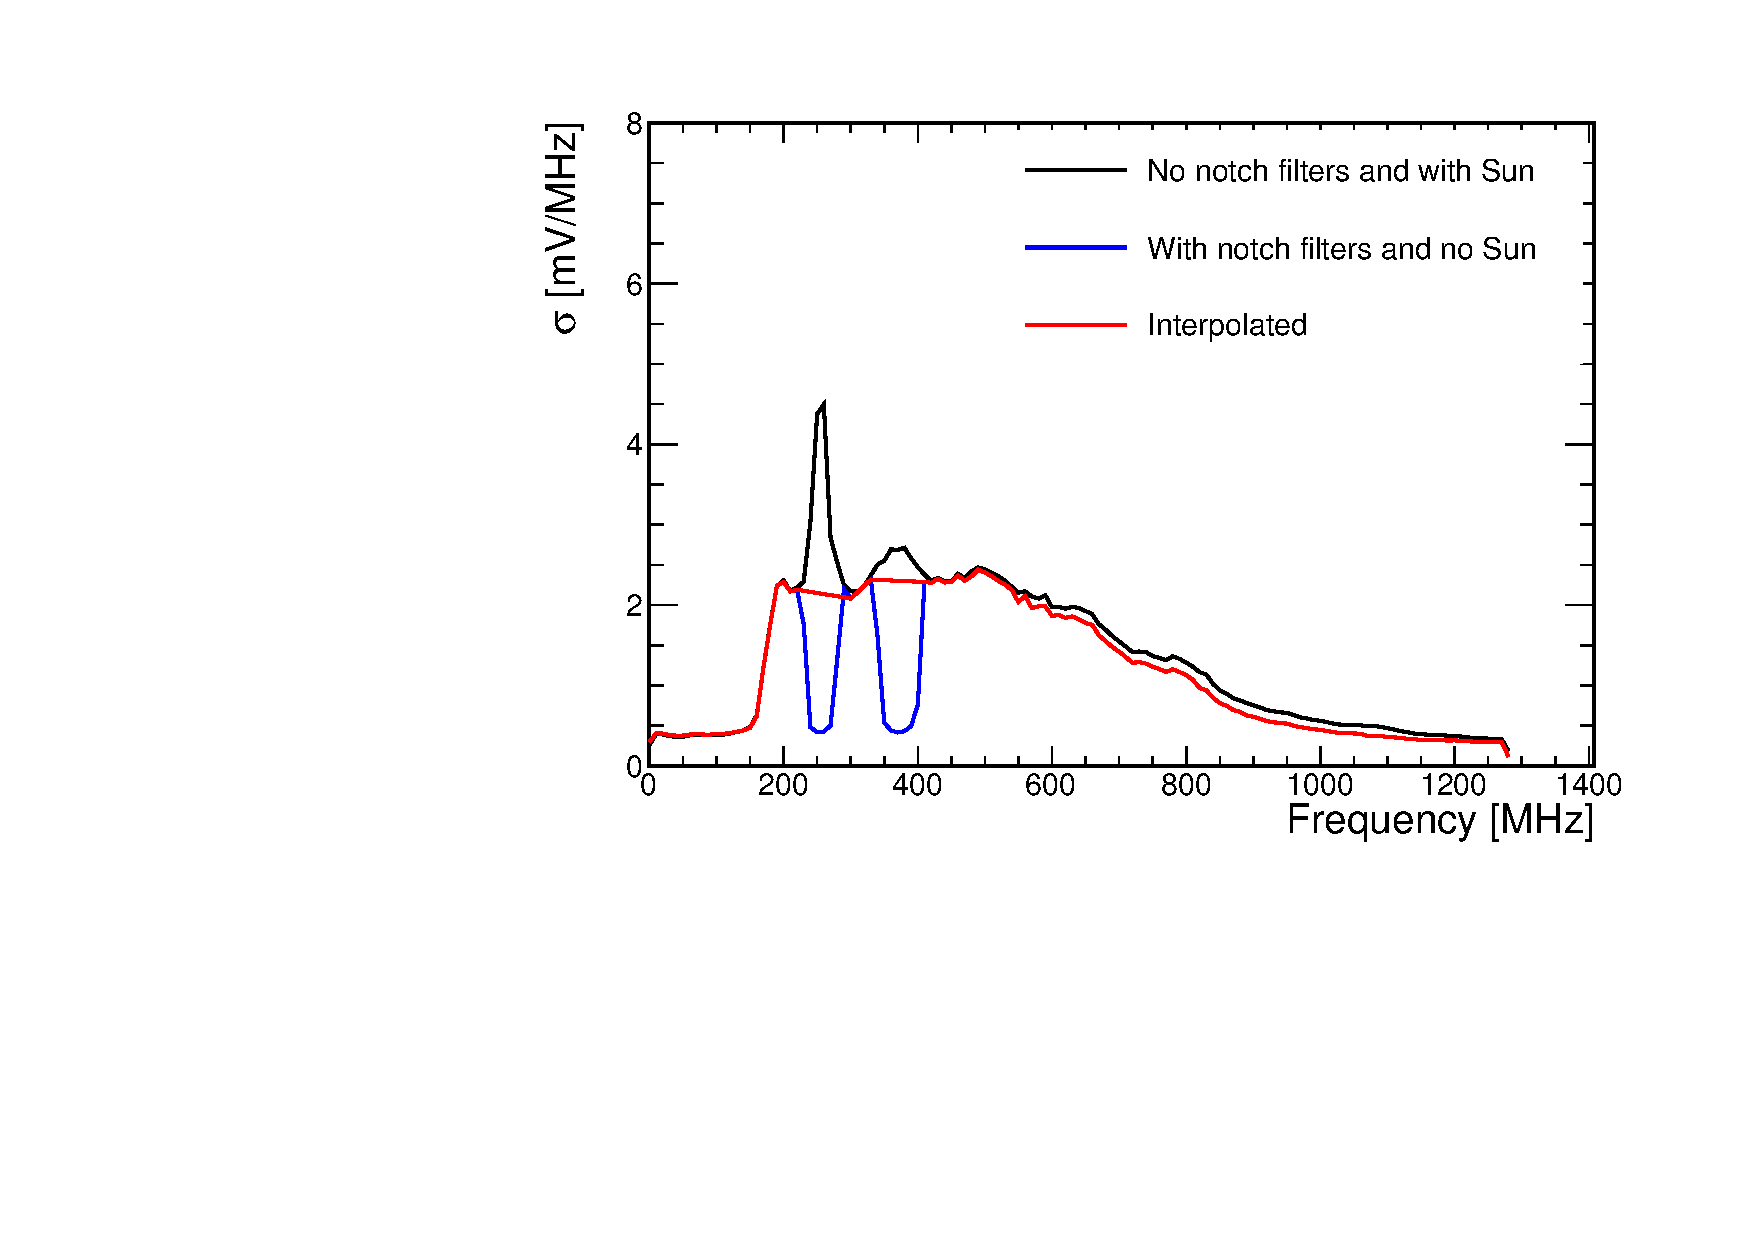
\includegraphics[width=.45\linewidth]{./Figs/RayleighSigma_1V_old.pdf}
  \caption{Example of a Rayleigh fit for a sample channel in the
    710.94\,MHz frequency bin (left). The fit is performed only to the rising edge and peak of the distributions, as most CW noise is in the tail. 
Right: fitted amplitude, $\sigma(f_i)$, as a
    function of frequency (interpolating in the frequency range where power is filtered). }
  \label{fig:rayleighFits}
\end{figure}

Graphs of the fitted amplitude, $\sigma(f_i)$, as a function of
frequency were produced for each channel (interpolating in the frequency range where power is filtered), as seen in Figure~\ref{fig:rayleighFits}(right).
In \icemc these graphs are used to generate random noise in the
frequency domain for each channel: for each frequency bin $f_i$ the real and imaginary part are randomly extracted from a Gaussian distribution with zero mean and amplitude
%\begin{equation} 
%  \begin{split}
%    \Re{f_i} & = RandomGaus(0, \sigma(f_i))/\sqrt{N_f} \\
%    \Im{f_i} & = RandomGaus(0, \sigma(f_i))/\sqrt{N_f} \\
%  \end{split}
%  \label{eq:thermalNoise}
%\end{equation}
%\noindent where $f_i$ is a frequency bin,
$\sigma(f_i)$, the fitted Rayleigh amplitude in that bin.
%and $N_f$ is the total number of frequencies.

This noise is added to the signal in the digitizer path.
For the trigger path the noise is re-normalized using the bin-by-bin ratio of the
trigger to digitizer path impulse response in the frequency domain
before adding it to the signal.

Thermal noise for the ANITA-IV simulation is derived from the ANITA-III measurements, accounting for the different electronics response (including the use of low noise amplifiers and variable filter configurations during the flight) for the two missions.
Samples containing only thermal noise are also produced, and they are used in
the main ANITA analyses to test the robustness of our analysis selection.
Subsection~\ref{subsec:validation_flight} details the thermal noise validation for both ANITA flights.

%While producing Rayleigh fits to all channels, it turned out that two
%channels (T04V and T04H) showed a different behavior than all the
%others, as shown in Figure~\ref{fig:noiseWeird}.
%T04V showed very irregular behavior during the whole flight (coming
%off and on at different periods), while T04H is the channel with the
%ALFA antenna attached to it, hence all frequencies above 700\,MHz were
%filtered out.
%For the moment these two graphs are used to simulate thermal noise in these two
%channels for the ANITA-III flight. 
%\begin{figure}[!h]\centering
%  \includegraphics[width=.45\linewidth]{/Users/linda/ANITA/anita3/anitaBuildTool/RandomMacros/powerSpectra/plots/RayleighSigma_4V.png}\,
%  \includegraphics[width=.45\linewidth]{/Users/linda/ANITA/anita3/anitaBuildTool/RandomMacros/powerSpectra/plots/RayleighSigma_4H.png}
%  \caption{Graphs of the fitted amplitude ($\sigma(f_i)$) as a
%    function of frequency for channels T04V and T04H (interpolating
%    between filtered frequencies).}
%  \label{fig:noiseWeird}
%\end{figure}

%\subsection{Anthropogenic noise} 
%\label{subsec:ANITA_anthropogenicNoise}



\subsection{Trigger simulation}
\label{subsec:ANITA_trigger}
The simulation models the L0 trigger by passing the
trigger-path signal through a time-domain tunnel diode model and comparing it to the
appropriate threshold from the flight for that channel at the event
time.
The tunnel diode response can be thought of as an integral of the power over about 10\,ns, but the true response is non-trivial.
The tunnel diode response function is constructed based on the
measured diode output for each channel.
The shape of the diode response is described by the sum of two negative Gaussians and a positive function that is the product of a quadratic and an exponential:
\begin{equation}
      f(t) = A_1 \cdot e^{-(t-t_0^1)^2/2\sigma_1^2} + 
      A_2 \cdot e^{-(t-t_0^2)^2/2\sigma_2^2} +
      A_3 \cdot \left( t-t_0^3 \right)^2 \cdot
      e^{-(t-t_0^3)/\sigma_3} \;,
    \end{equation}
\noindent where the values for the parameters used for all channels are shown in
Table~\ref{tab:diodeModelParameters};
$f(t)$ is dimensionless.
%Reference~\cite{diodeModel} describes how the model was found. 
Figure~\ref{fig:ANITA_diodeModel} shows the diode response model function.

\begin{table}[h!]
\caption{Tunnel diode model parameters used for the full band trigger in ANITA-III and ANITA-IV.}
  \begin{center}
    \begin{tabular}{c|c|c|c} 
      & Value 1 & Value 2 & Value 3 \\
     \hline
      $A$           & -0.8  & -0.2   &  0.00964   \\
      $\sigma$ [ns] &  2.3  &  4.0   &  7.0       \\ 
      $t_0$  [ns]   & 15.0  & 15.0   & 18.0       \\
    \end{tabular}
  \end{center}
  \label{tab:diodeModelParameters}
\end{table}


\begin{figure}[!h]\centering
  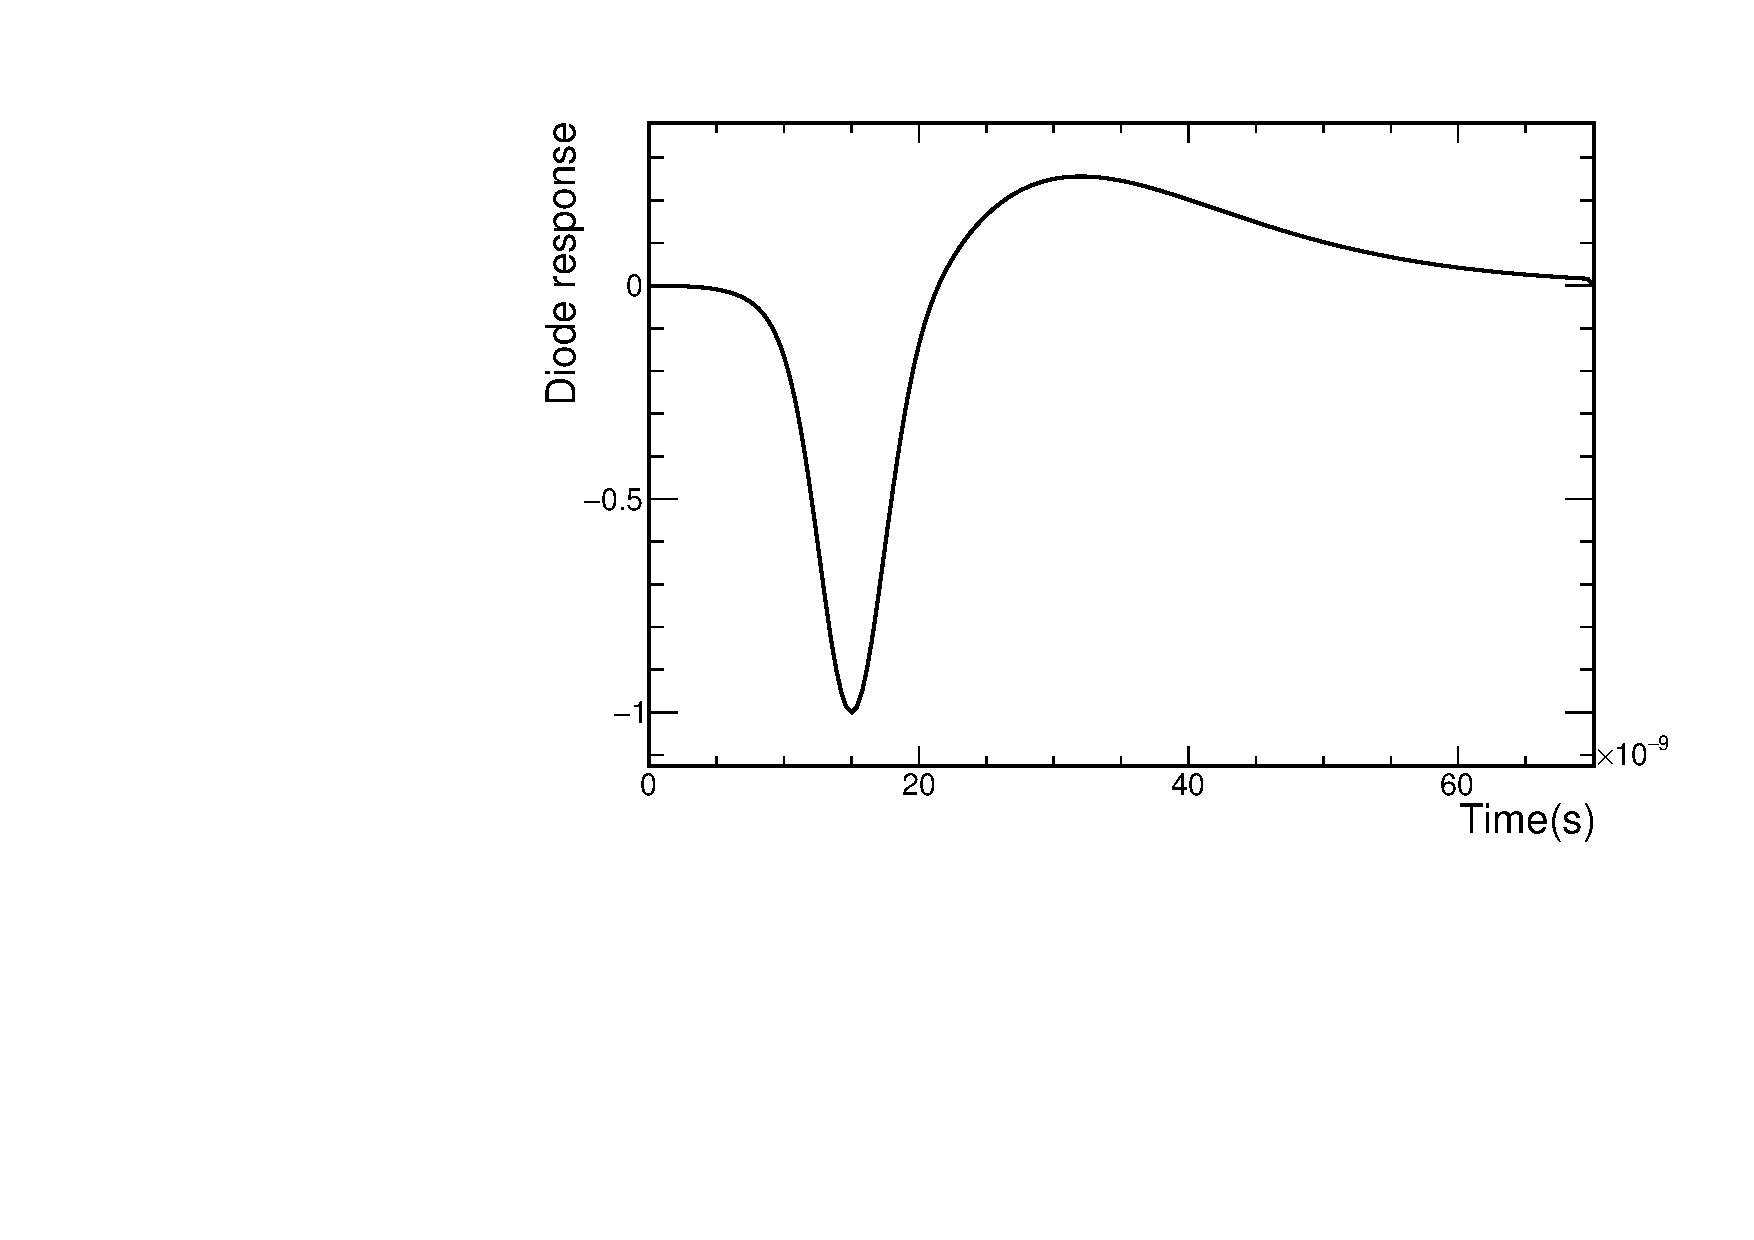
\includegraphics[width=.45\linewidth]{./Figs/FullBand_diodeResponse.pdf}
  \caption{Tunnel diode response model used in \icemc.}
  \label{fig:ANITA_diodeModel}
\end{figure}

For each signal, the power as a function of time is calculated as:
\begin{equation}
  P (t) = \dfrac{V(t) \cdot V(t)}{Z} \;,
\end{equation}
\noindent where $V(t)$ is the voltage at time $t$, and $Z=50\,\Omega$ is the system impedance.
The next step is to convolve the waveform power with the diode
response to find the diode output $D(t)$:
\begin{equation}
  D(t) = (f * P)(t) \;.
\end{equation}
For each time bin, the diode output is compared to the channel
threshold, $V_T$, multiplied by the RMS voltage of the diode outputs coming from pure thermal noise, $V_{RMS}$, following:
\begin{equation} 
  D(t) < V_T \cdot V_{RMS} \;.
\end{equation}
If the power output is more negative than the threshold multiplied by $V_{RMS}$ at any point, then that channel passes the L0 trigger.
  See Figure~\ref{fig:ANITA_diodeOutput} for an example of diode
  output that does not pass the L0 trigger (left) and that does pass
  the L0 trigger (right).

\begin{figure}[!h]\centering
  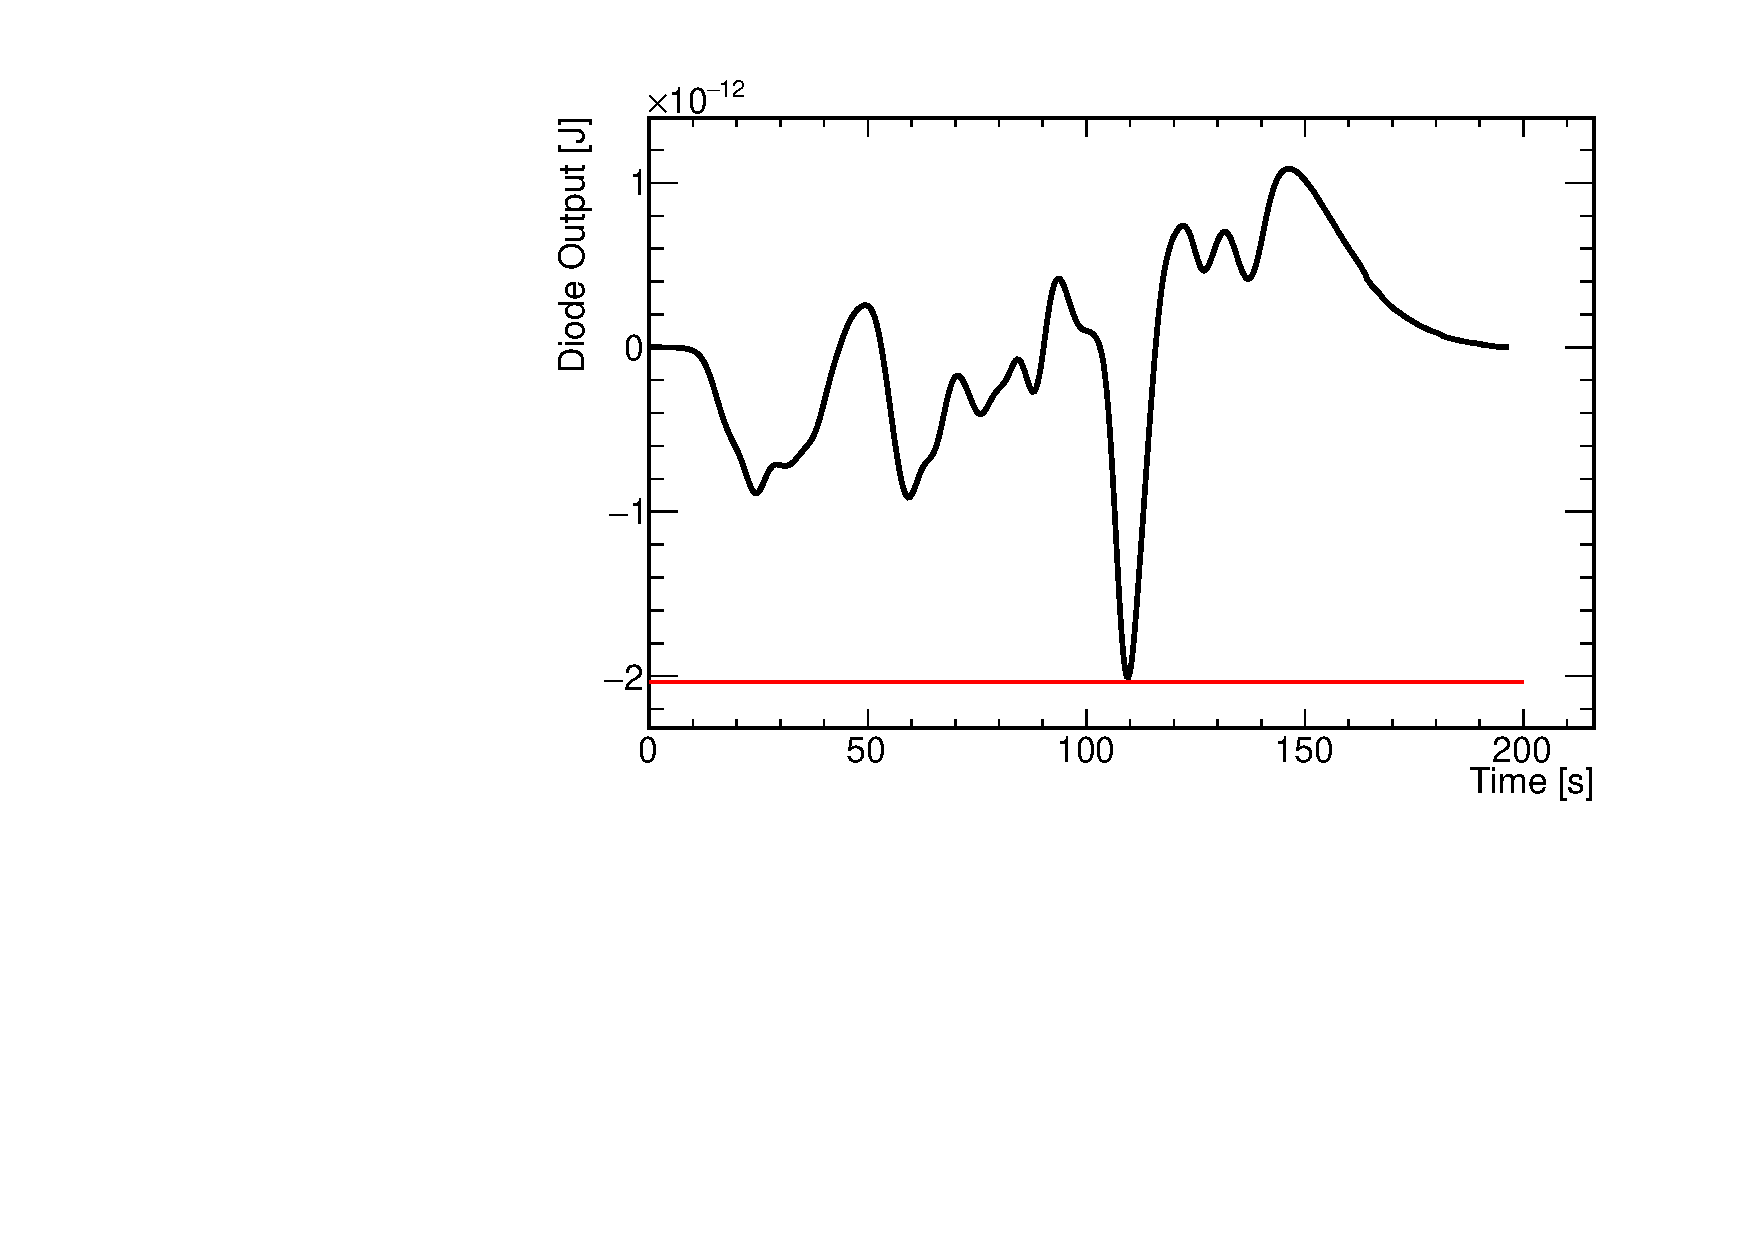
\includegraphics[width=.45\linewidth]{./Figs/ExampleDiodeOutput_NOpass.pdf}
  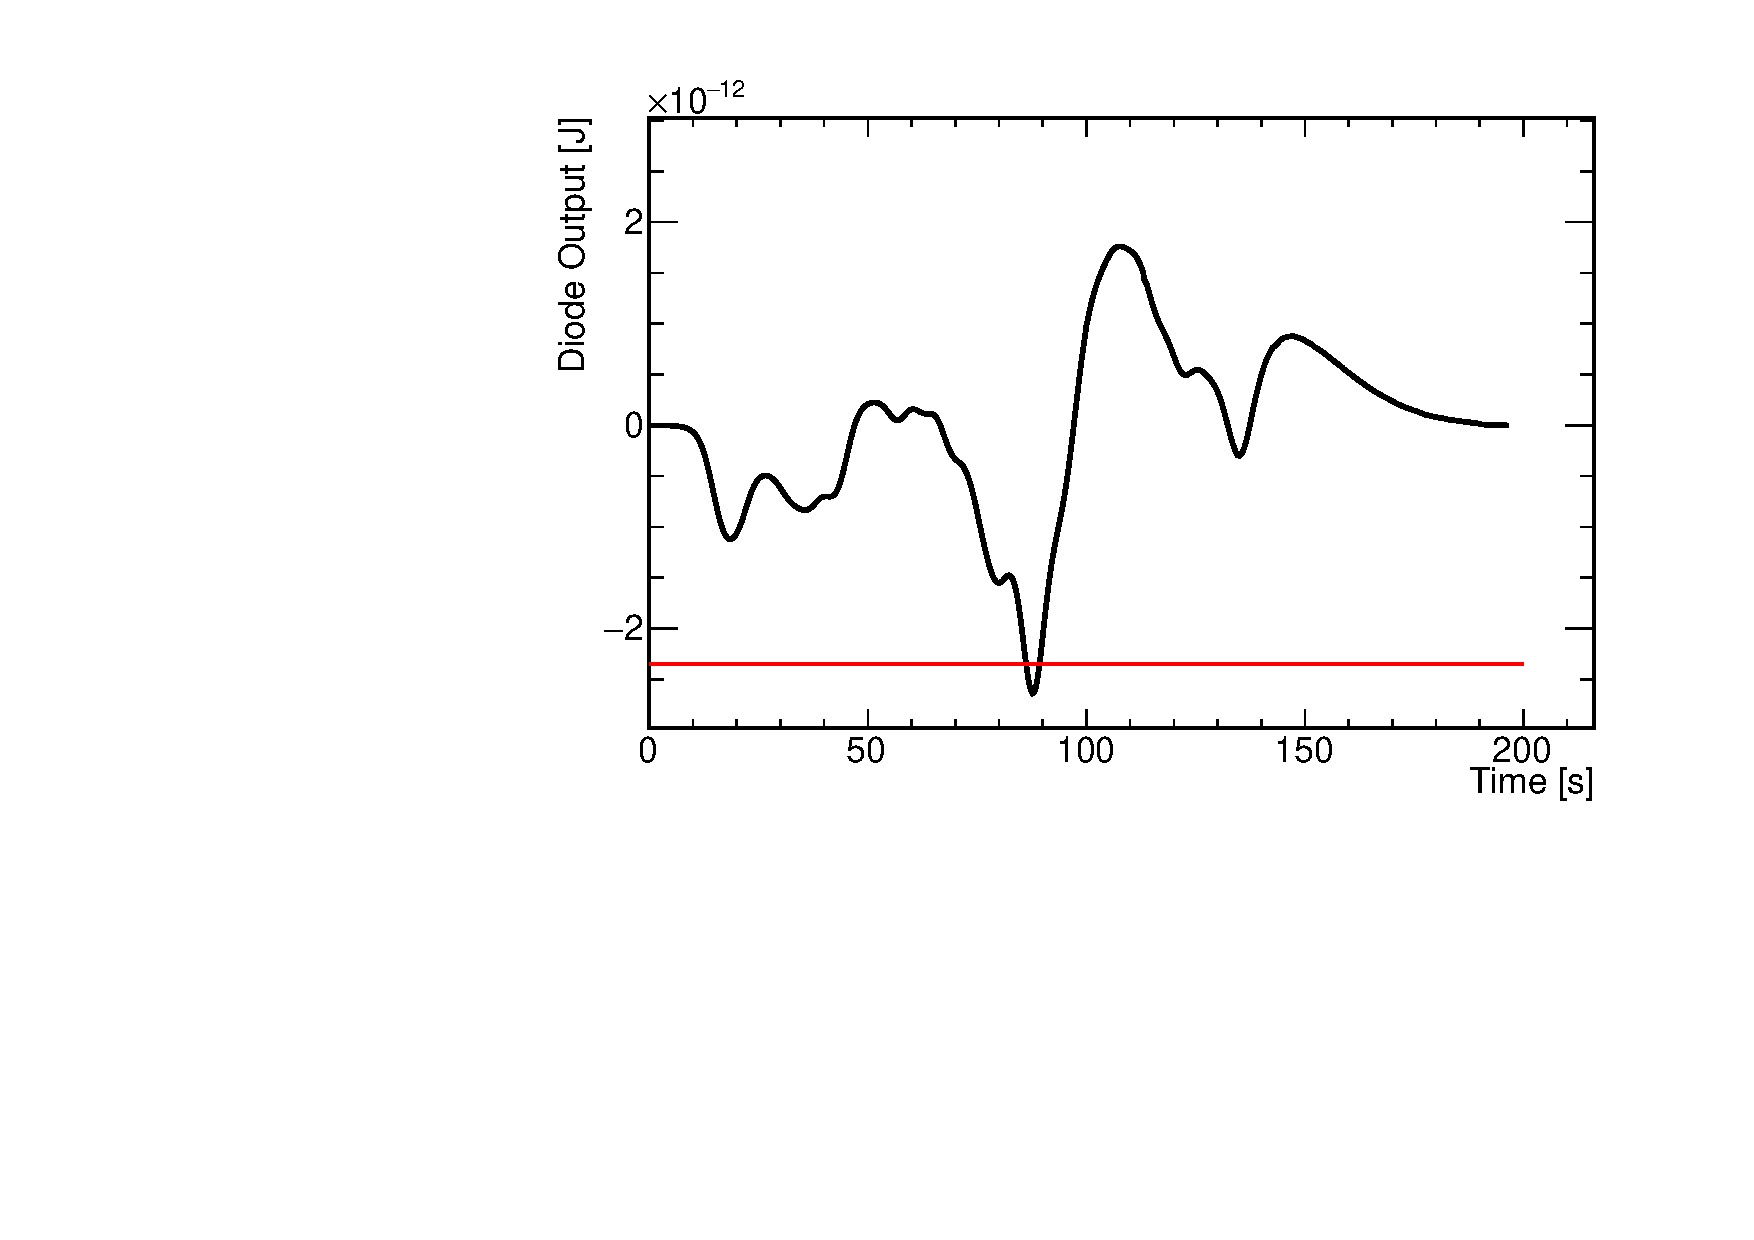
\includegraphics[width=.45\linewidth]{./Figs/ExampleDiodeOutput_pass.pdf}
  \caption{Example of diode output that does not pass the L0 trigger (left) and that does pass the L0 trigger (right). The red
    line shows the value of $V_T \cdot V_{RMS}$, showing that the
    waveform on the right passes the L0 trigger and the waveform on
    the left does not.}
  \label{fig:ANITA_diodeOutput}
\end{figure}

At the beginning of a run, $V_{RMS}$ is calculated for each channel 
by simulating 1000 noise waveforms
(Subsection~\ref{subsec:ANITA_thermalNoise}) 
and sampling the diode output at the center of each waveform
(see Figure~\ref{fig:ANITA_diodeRMS}).
In ANITA-III, two channels had very large $V_{RMS}$ associated with them that prevents them from triggering in the simulation: one was broken during the flight, and the other one had an additional filter applied during flight to
allow an in-flight calibration pulser to be used.

\begin{figure}[!h]\centering
  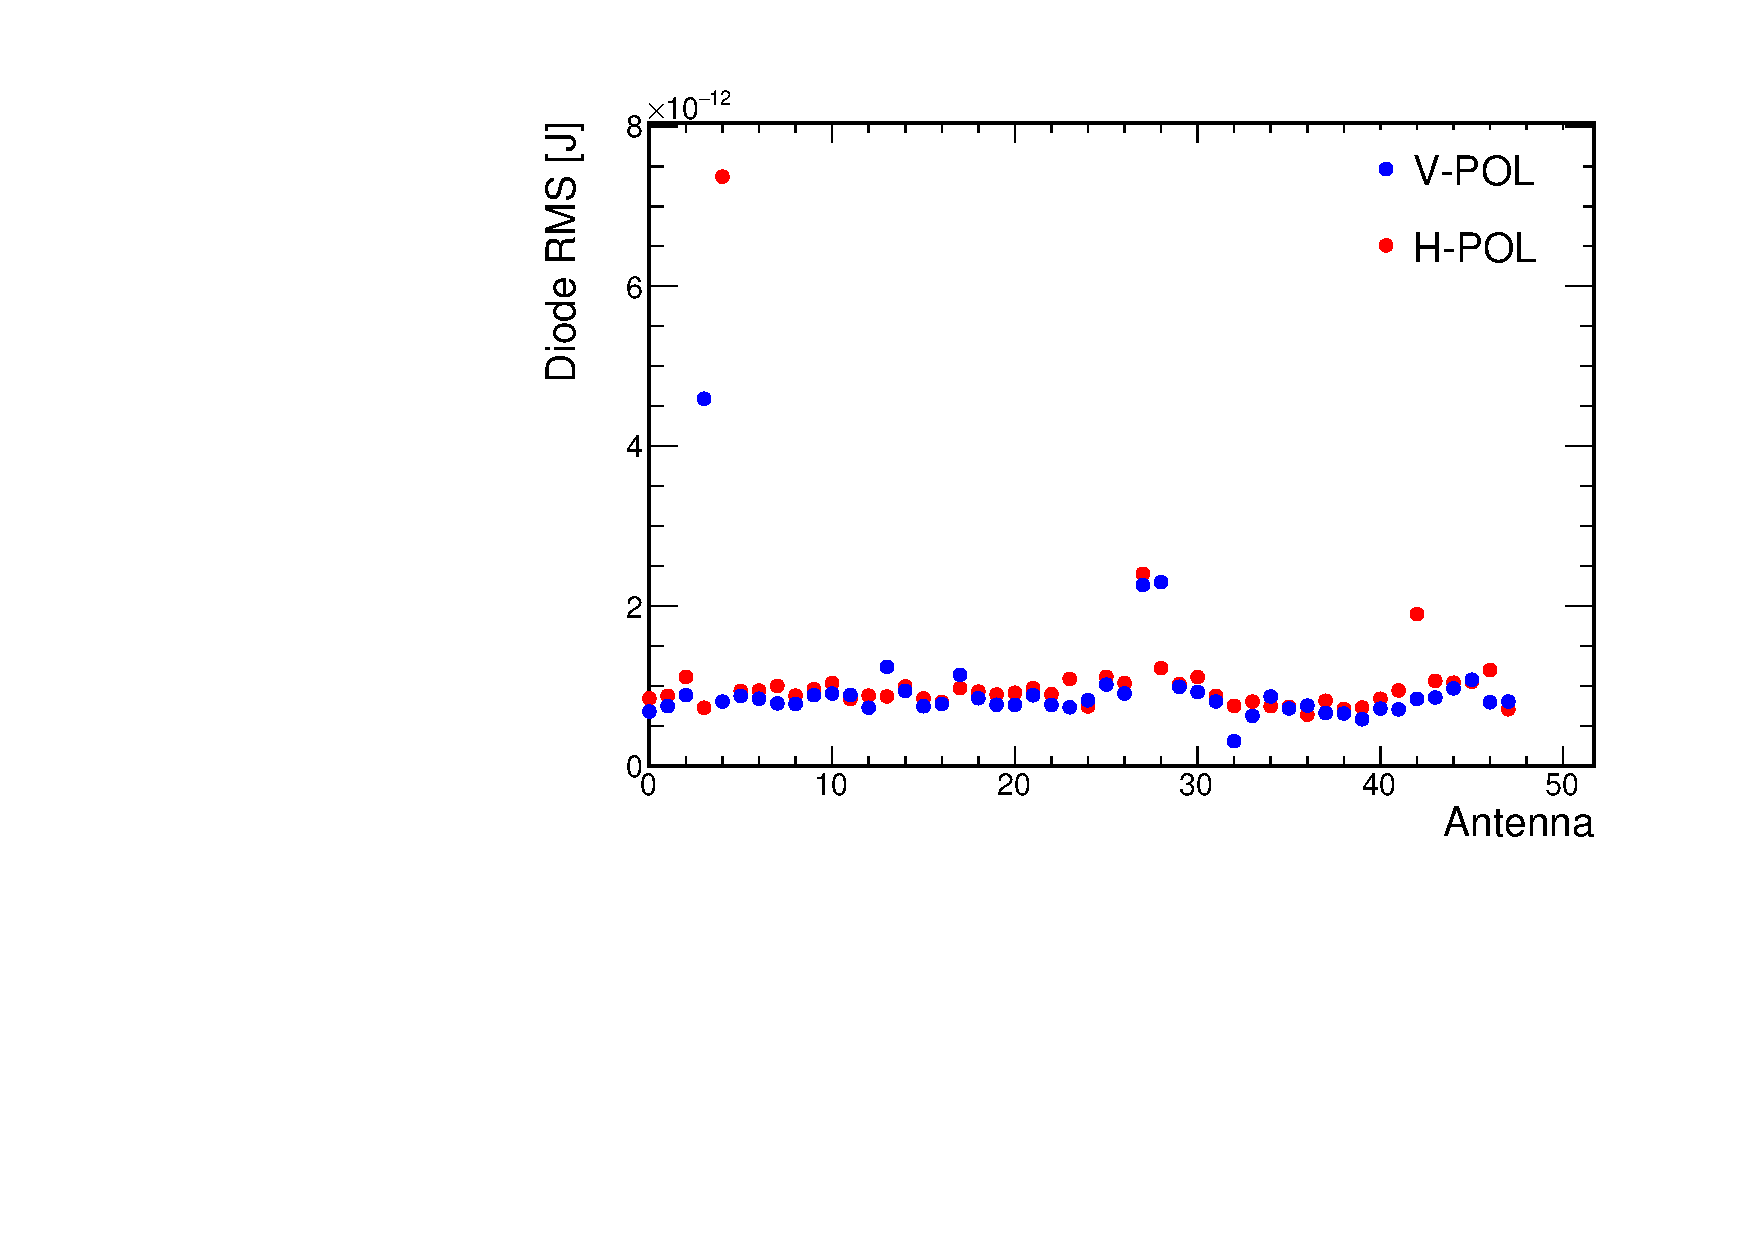
\includegraphics[width=.45\linewidth]{./Figs/DiodeRMSfromFile.pdf}
  \caption{Tunnel diode $V_{RMS}$ for each channel. The two channels with much higher $V_{RMS}$ are the broken channel, and the channel which had an additional filter applied to accommodate the use of an in-flight calibration system.}
  \label{fig:ANITA_diodeRMS}
\end{figure}
 
The trigger logic for the ANITA-III and ANITA-IV triggers is very similar.
The main difference is that ANITA-IV used 90 degree hybrids to transform HPOL and VPOL signals into LCP and RCP components of waveforms, so the ANITA-IV L1 trigger requires a LCP and RCP L0 coincidence in the same antenna within one 4\,ns clock cycle.
The ANITA-III instrument did not have an L1 trigger.
The L2 trigger is formed by a coincidence of two out of three
antennas (top, middle, bottom) in the same azimuthal
sector. As ANITA is intended to look for plane-waves from below, a simple
causal requirement is enforced on the coincidence windows.  An L1 on the bottom
antenna opens a coincidence window open for four FPGA clock cycles (nominally 16\,ns).
Middle and top L1's open the window for three and one-clock cycles (nominally 12 and 4
ns), respectively (see
Figure~\ref{fig:ANITA_triggerLogic} (left)).  
Finally, the global trigger is formed by the coincidence of L2 triggers in
two adjacent azimuthal sectors (see Figure~\ref{fig:ANITA_triggerLogic} (right)) within 3 clock cycles.
For ANITA-III either polarization or both may produce a global trigger. 
Either the L2 or global-trigger may be masked for an
azimuthal sector if the L2 or global rate is too high in the sector.
The actual time-dependent masking status from the flight is used in the simulation.


\begin{figure}[!h]\centering
  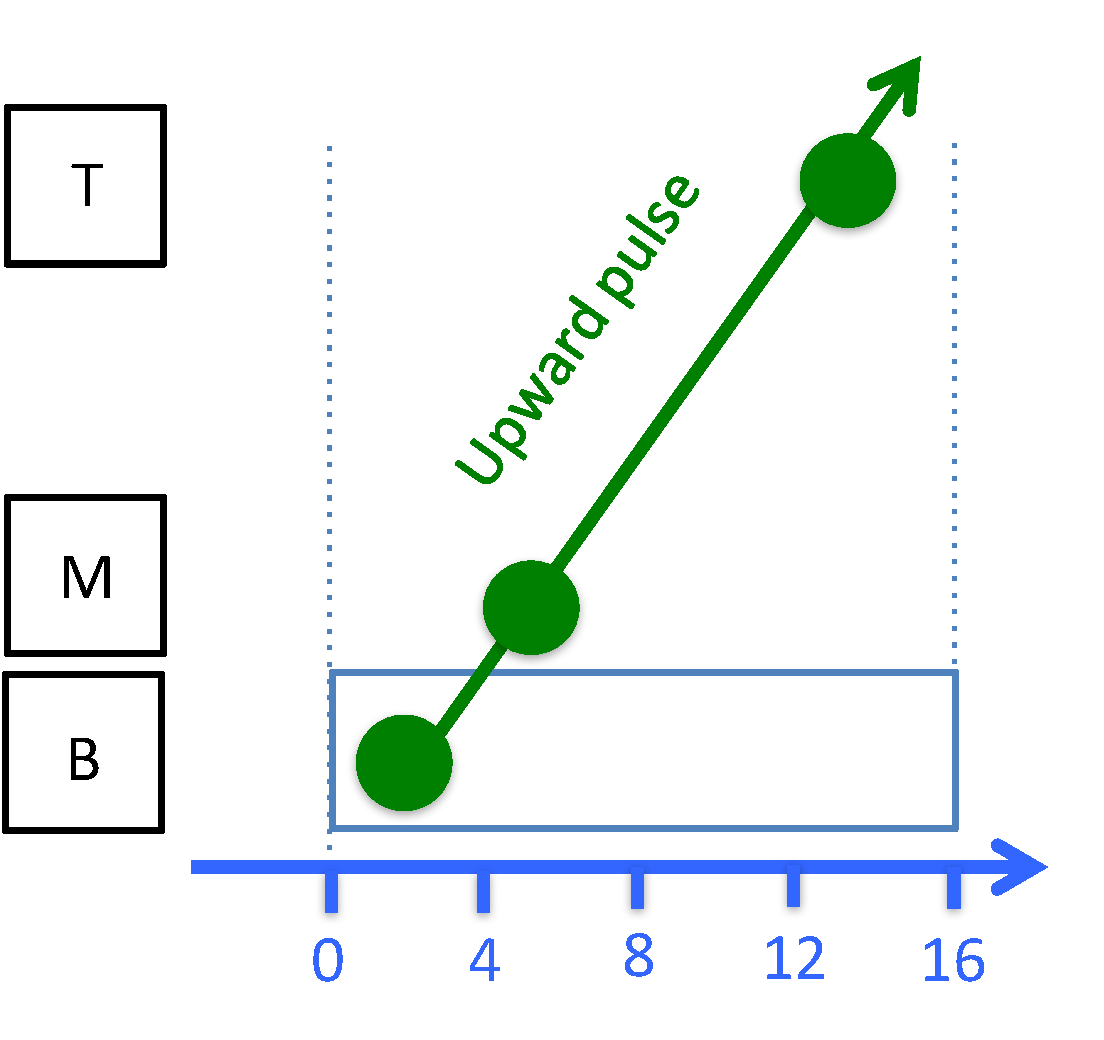
\includegraphics[width=.45\linewidth]{./Figs/ANITA3_l1trigger.pdf}
  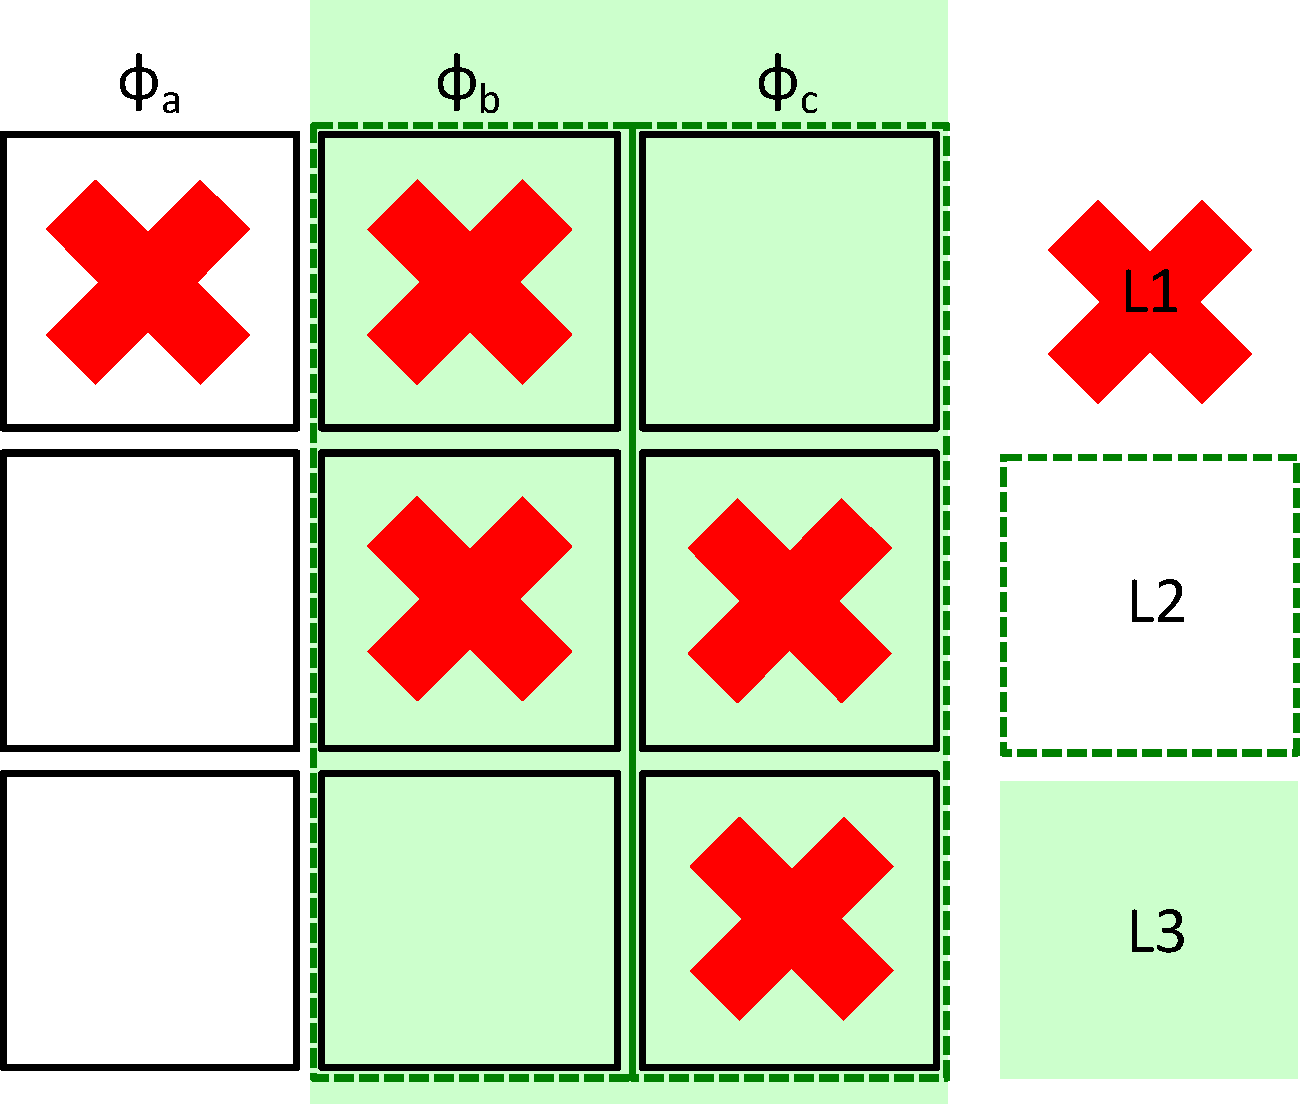
\includegraphics[width=.45\linewidth]{./Figs/ANITA3_globalTrigger.pdf}
  \caption{Schematic of a second-level trigger example (left), where a
  plane-wave triggers an antenna in the bottom ring first, and a
  16\,ns window is opened to check L1 triggers in the middle and top
  ring.
The diagram on the right shows the issuance of a global trigger when two
adjacent azimuthal sectors had an L2 trigger.}
  \label{fig:ANITA_triggerLogic}
\end{figure}




%\subsubsection{Time dependent thresholds}
%\label{subsubsec:ANITA_thresholds}
%The ANITA-III flight softwares used an algorithm to vary the channel power thresholds during the flight and avoid overloading the DAQ in
%regions where the anthropogenic noise was higher.
%This algorithm tried to keep the scalers at roughly 500\,kHz.
%The current version of \icemc does not include anthropogenic noise or thermal variation coming from the Sun, but we still need to simulate the power threshold changes to have a more accurate simulation of our flights.

%In \icemc for every event, when picking the balloon position, the
%scalers for each channel are set by looking at sample data taken from the ANITA-III flight.
%The scalers are converted into relative power thresholds using
%a log function in the range 1-25\,MHz, assuming an exponential diode
%model with time constant $3.75 \times 10^{-9}$\,s.
%This was calculated from a fit to single channel power thresholds taken with
%an oscilloscope in 2008.

%Section~\ref{sec:validation} shows the variation of the acceptance when using the time-dependent thresholds or using constant thresholds throughout the simulated flight.

%Future versions of \icemc will include the simulation of anthropogenic noise, the contribution of the Sun, and a better treatment of the time varying thresholds.





\section{Validation}
\label{sec:validation}
Different parts of the simulation are validated from measurements
taken in the lab (Subsection~\ref{subsec:validation_lab}) and during
the flights (Subsection~\ref{subsec:validation_flight}).


\subsection{Comparisons with lab measurements}
\label{subsec:validation_lab}
Before each of the ANITA flights a series of calibration measurements was
taken at the NASA Long Duration Balloon Facility near McMurdo Station, Antarctica.
These measurements are used to cross-check different parts of the simulation.

\subsubsection{Trigger efficiency scans}
\label{subsec:validation_scans}
Trigger efficiency scans are used to measure the ANITA trigger efficiency
for signals with different signal-to-noise ratios (SNRs).
The setup used before the ANITA-III flights is shown in Figure~\ref{fig:scan_setup}. 
A Picosecond Pulse generator is used to produce an RF signal. 
This is recorded with an oscilloscope and fed directly into the
amplifiers  behind the ANITA antennas (after going through some attenuators and a 12-way splitter).
Six of these channels are sent through the trigger and digitizer paths of
two azimuthal sectors and
are used to measure the global trigger efficiency. 
One is fed back into the oscilloscope to measure the SNR values.

\begin{figure}[!h]\centering
  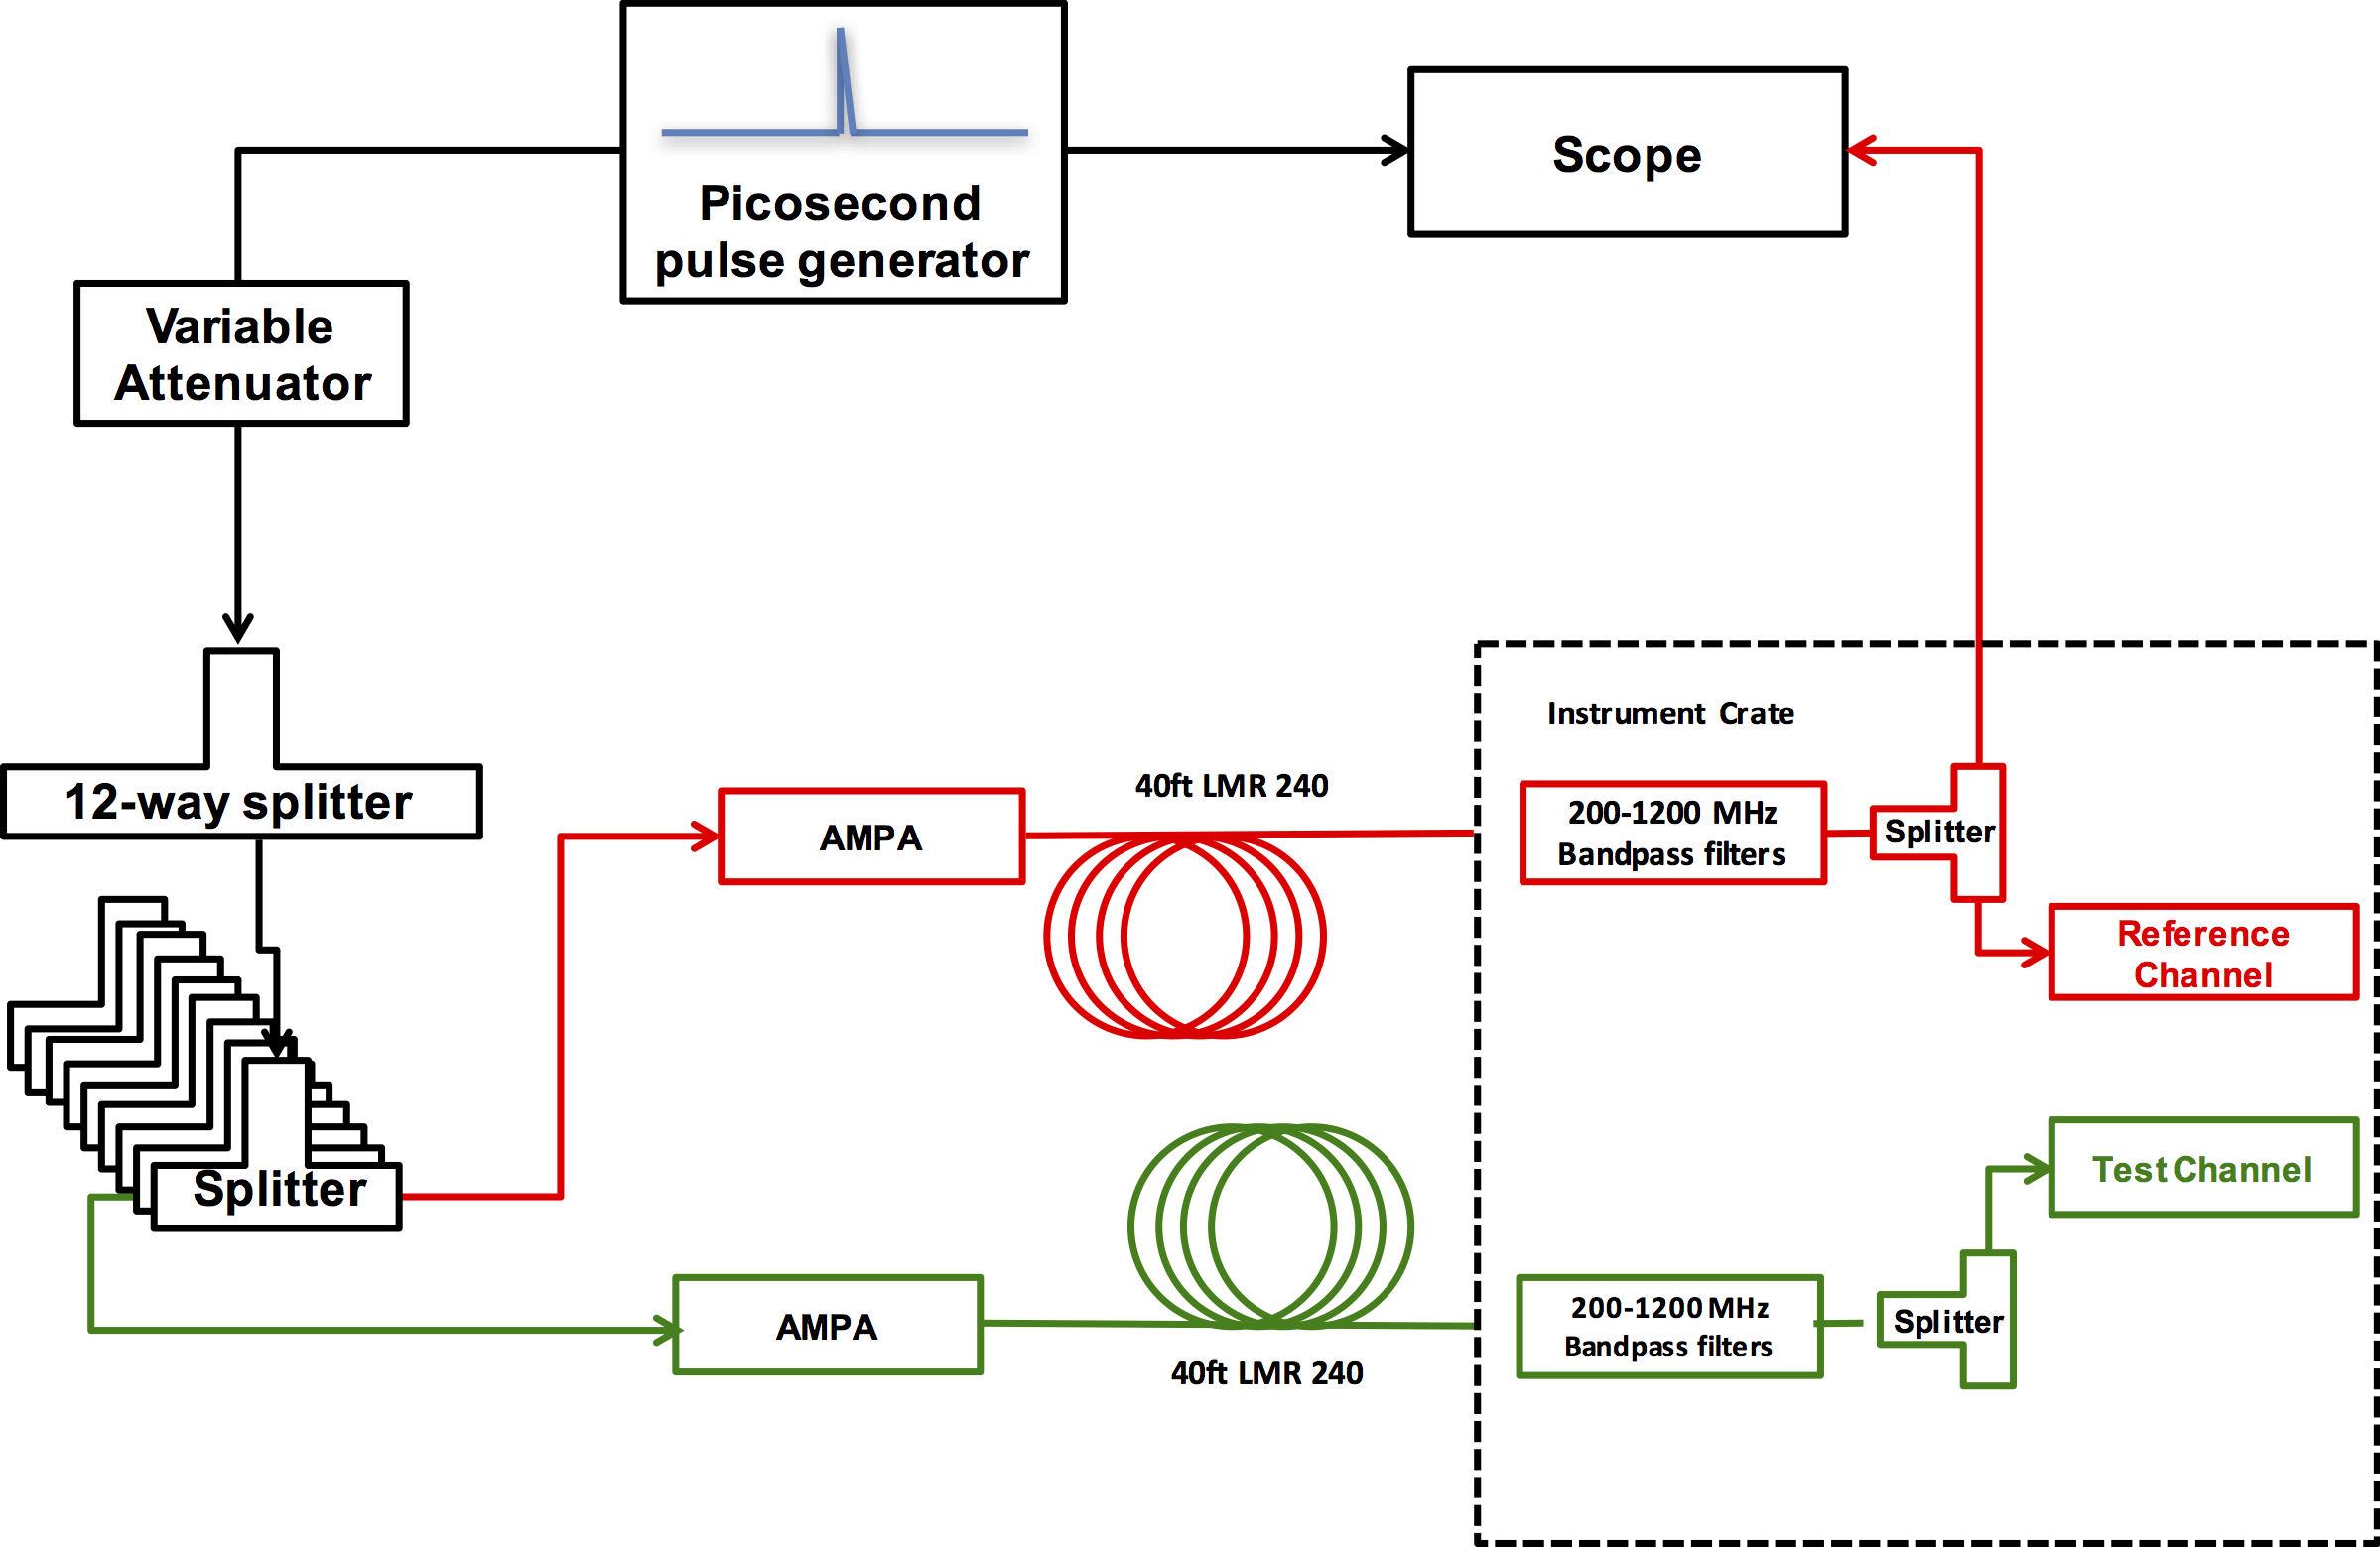
\includegraphics[width=.8\linewidth]{./Figs/TriggerEfficiencyScanSetup.png}
  \caption{Trigger efficiency scans setup in Antarctica before the ANITA-III flight.}
  \label{fig:scan_setup}
\end{figure}

%See Figure~\ref{fig:scan_waveforms} for examples of the RF signals measured by the oscilloscope during a trigger efficiency scan.
%\begin{figure}[!h]\centering
%  \includegraphics[width=.45\linewidth]{./Figs/Comparison_inputWaveform.png} \,
%  \includegraphics[width=.45\linewidth]{./Figs/Comparison_finalWaveform.png}
%  \caption{Left: RF signal as generated by the pulser and read in by \icemc.
%  Right: Example RF signal as read in by the oscilloscope after having passed through the trigger path compared to what is simulated in \icemc.
%  {\color{red}LINDA: Make better plots}}
%  \label{fig:scan_waveforms}
%\end{figure}

%A custom program, {\tt testInputAfterAntenna}, can be used to test the
%ANITA instrument model response on any inputs injected behind the antennas.
To simulate the trigger efficiency scan setup, the signals
measured at the oscilloscope (see Figure~\ref{fig:scan_setup}) are
injected into the same six channels used in the data scans, after
appropriate attenuation is applied.
These go through the trigger/digitizer path and produce ANITA
data-like outputs.
When simulating trigger efficiency scans, constant power
thresholds corresponding to 450\,kHz scalers are used for all channels.

The signals are recorded at the trigger (red line going to the
oscilloscope in Figure~\ref{fig:scan_setup}) and the digitizer paths
are used to validate the simulation.
Figure~\ref{fig:scan_snr} shows a comparison between data and \icemc
of the SNR measured at the trigger (left)
and at the digitizer (right) as a function of the variable attenuation used
during the scan.
The measured SNR in the digitizer path has generally higher errors compared to the SNR in the trigger path, because the ANITA digitizer has on average a
2.6\,GHz sampling rate, whereas the trigger path is measured with a
fast oscilloscope. 

\begin{figure}[!h]\centering
  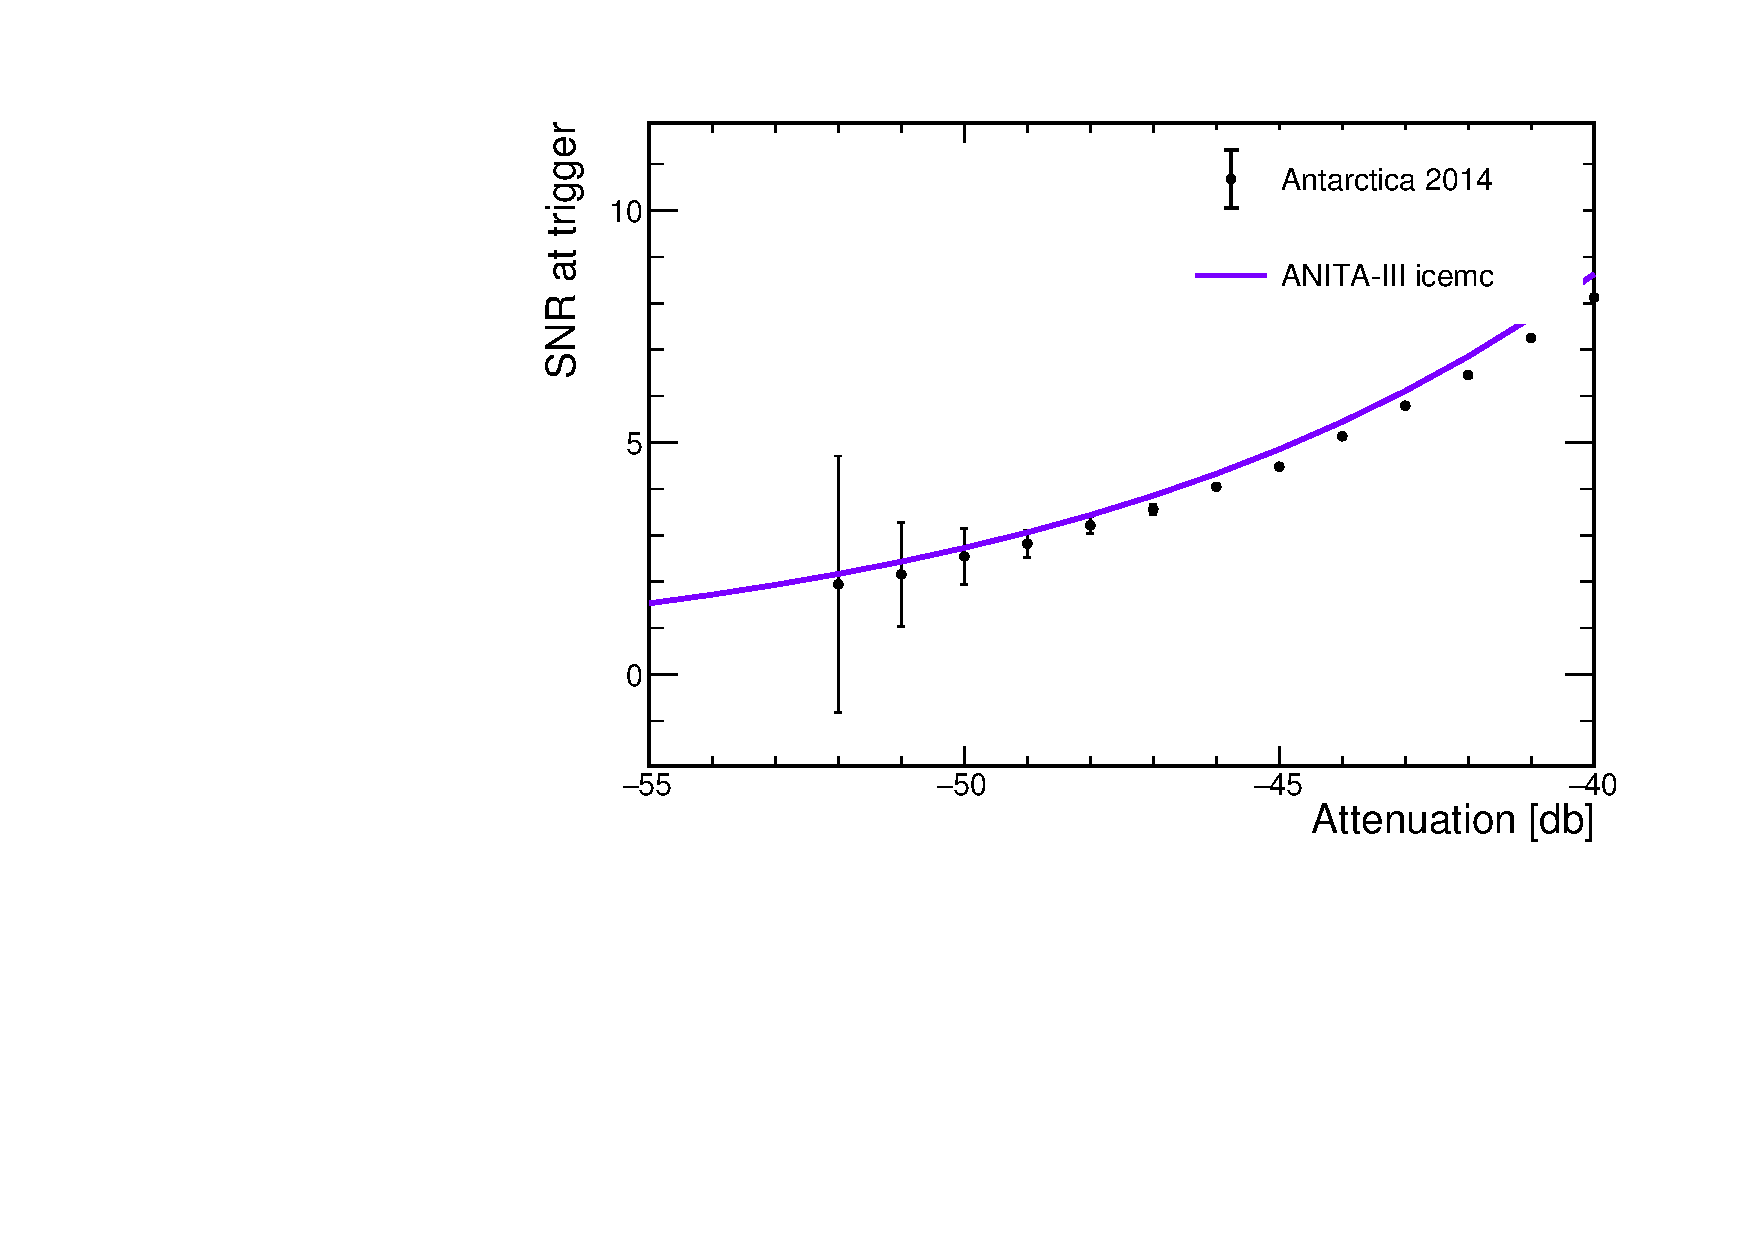
\includegraphics[width=.45\linewidth]{./Figs/EfficiencyScanNoDelaysA3_snrTriggerVSattenuation.pdf} 
  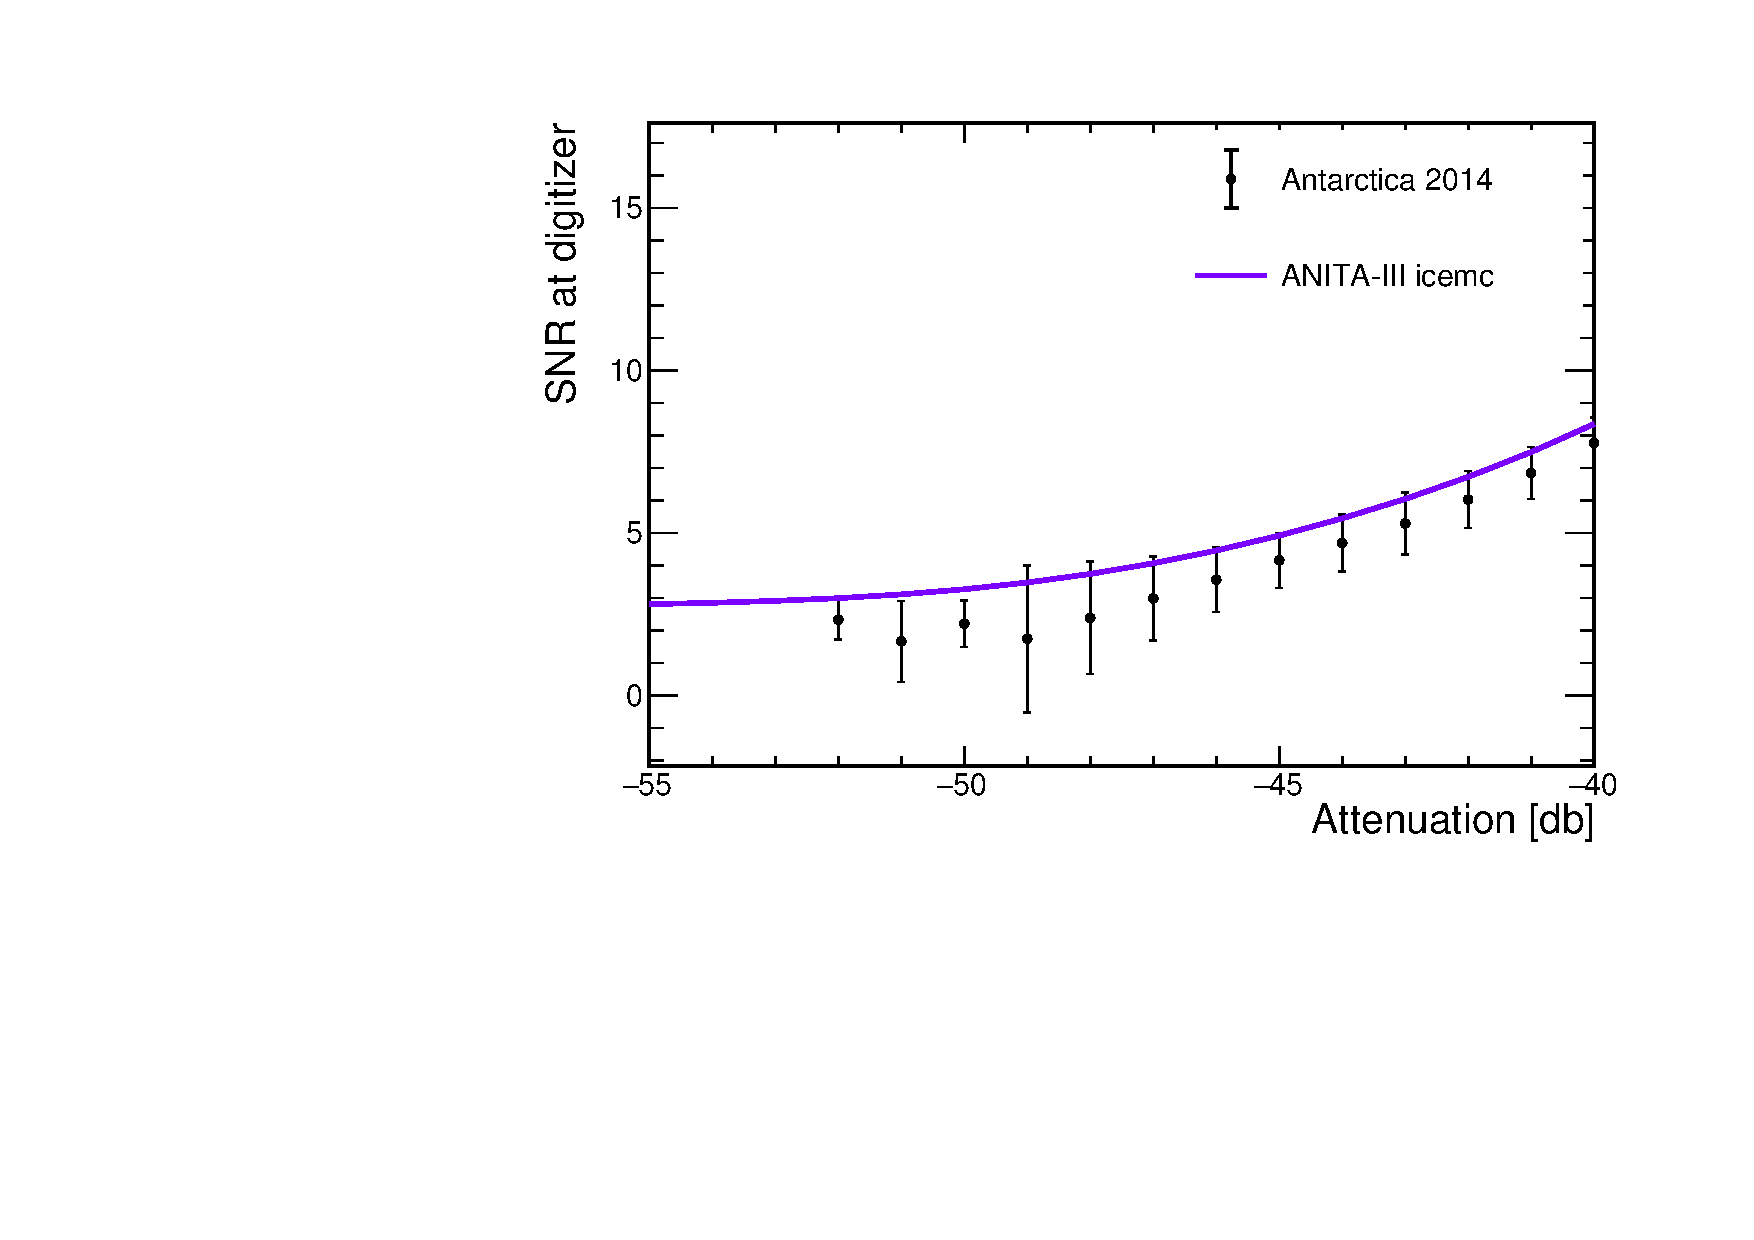
\includegraphics[width=.45\linewidth]{./Figs/EfficiencyScanNoDelaysA3_snrDigitizerVSattenuation.pdf}
  \caption{SNR measured at the trigger (left) and digitizer (right) as
  a function of the variable attenuation applied during the trigger
  efficiency scans. The data points were measured in 2014 in Antarctica prior to the
  ANITA-III flight.
}
  \label{fig:scan_snr}
\end{figure}

Figure~\ref{fig:scans}(left) shows a data and simulation comparison of a trigger
efficiency scan for the ANITA-III payload.
The trigger efficiency is plotted a function of the SNR
measured in the trigger path.

Before the ANITA-IV flight (Antarctica 2016), a similar set of measurements was collected at a 6\,MHz rate. 
A data and simulation comparison of the trigger efficiency for the ANITA-IV instrument is shown in Figure~\ref{fig:scans}(right).

\begin{figure}[!h]\centering
  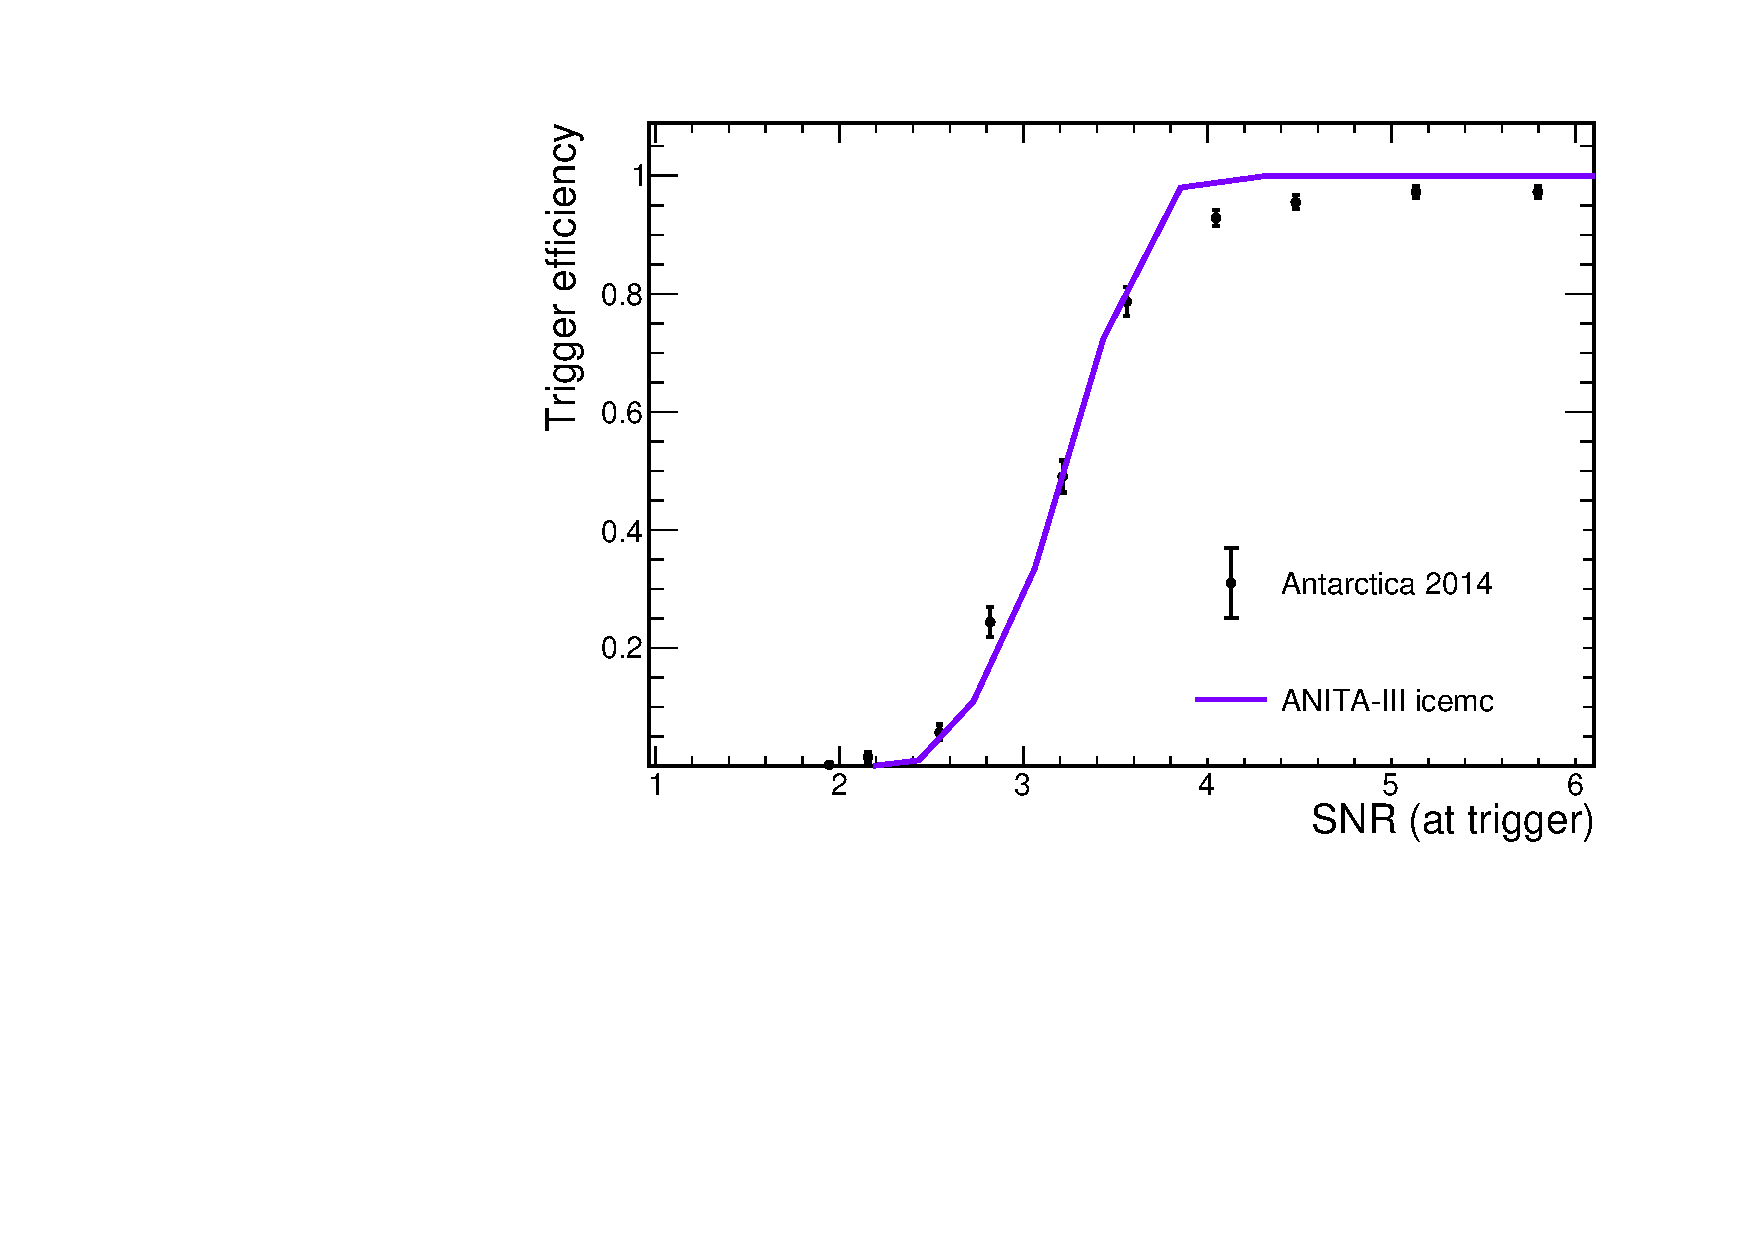
\includegraphics[width=.45\linewidth]{./Figs/EfficiencyScanNoDelaysA3_efficiencyVSsnrTrigger.pdf}
    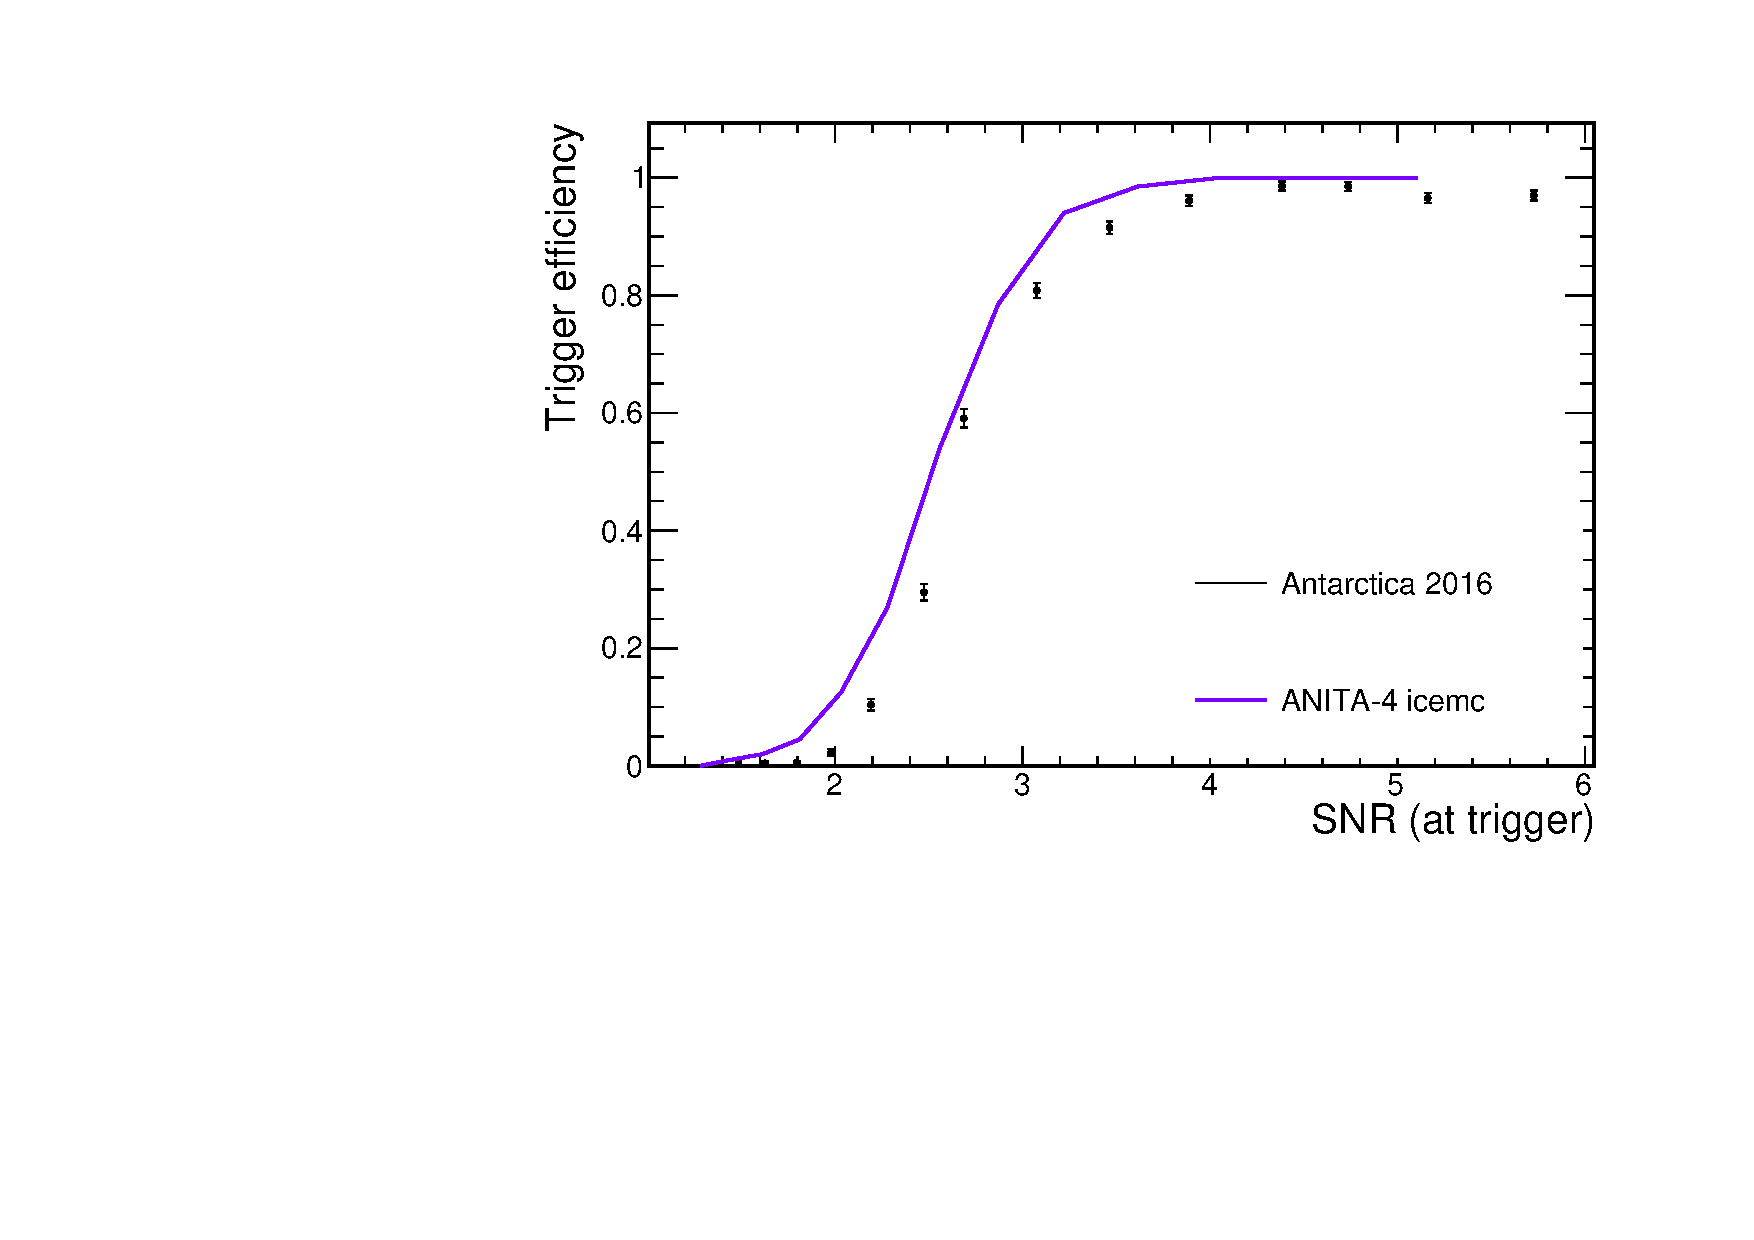
\includegraphics[width=.45\linewidth]{./Figs/EfficiencyScanNoDelaysA4_efficiencyVSsnrTrigger.pdf}
  \caption{Data and simulation comparison of a trigger efficiency scan for the ANITA-III (left) and ANITA-IV (right) instruments. 
    The trigger efficiency is plotted a function of the SNR
    measured at the oscilloscope for the data, and the SNR estimated in the trigger path for the simulation. 
    %\CD{Hmm, how come the left differs from what's in the A3 paper and the right differs from elog 691? Is it because there is no relative attenuation applied between the two sectors?}
    }
  \label{fig:scans}
\end{figure}

%In the same dataset we performed checks of the trigger coincidence
%windows between 2 phi sectors and different rings. 
%The first were done by injecting a pulse in 4 channels (2 rings and 2
%phi sectors) and delay one phi sector with respect to the other one.
%Figure~\ref{fig:scan_phidelay} shows the data and \icemc comparison of
%this scan: why delaying phi sector 16 with respect to 1 gives a larger
%plateau that delaying phi sector 16 with respect to 15. 
%Even though the MC has larger accepting windows than the data, this
%behavior seems to be reproduced.
%
%\begin{figure}[!h]\centering
%  \includegraphics[width=.65\linewidth]{./Figs/EfficiencyScanPhiDelay.pdf}
%  \caption{Data and MC comparison of a trigger efficiency scan for the
%    ANITA-III payload. Pulses were injected in two phi sectors and one
%    phi sector was delayed with respect to the other one.}
%  \label{fig:scan_phidelay}
%\end{figure}
%
%The other type was scan consists in checking the trigger ring
%coincidence windows. 
%This is done by injecting the pulse in 4 phi sectors, and delaying
%only one of them (see Figure~\ref{fig:scan_ringdelay}), or delaying
%both phi sectors in one ring with respect to the other ring (see
%Figure~\ref{fig:scan_ringdelay} bottom right).
%
%\begin{figure}[!h]\centering
%  \includegraphics[width=.45\linewidth]{./Figs/EfficiencyScanRingDelay_singleTM.pdf} 
%  \includegraphics[width=.45\linewidth]{./Figs/EfficiencyScanRingDelay_singleTB.pdf} \\
%  \includegraphics[width=.45\linewidth]{./Figs/EfficiencyScanRingDelay_singleMB.pdf}
%  \includegraphics[width=.45\linewidth]{./Figs/EfficiencyScanRingDelay_togetherTM.pdf}
%
%  \caption{Data and MC comparison of a trigger efficiency scan for the
%    ANITA-III payload. Pulses were injected in two phi sectors on two
%    different rings. One phi sector was delayed with respect to the
%    other 3 (top left, top right and bottom left), or both phi sectors
%    were delayed in one right with respect to the other (bottom right).}
%  \label{fig:scan_ringdelay}
%\end{figure}



\subsection{Comparisons with flight measurements}
\label{subsec:validation_flight}
Data taken during the ANITA-III and ANITA-IV flights is used to validate 
the thermal noise, the trigger efficiency to a ground pulser, and the pointing reconstruction.

\subsubsection{Thermal noise validation}
\label{subsec:ANITA_validation_thermalNoise}
The digitized thermal noise is validated using distributions of
the RMS of the simulated waveforms compared to a relatively quiet time
during the flights.
The ANITA-III quiet time is defined in Subsection~\ref{subsec:ANITA_thermalNoise}); for the ANITA-IV quiet time, we used forced triggers from run 200.
Figure~\ref{fig:RMSwaveform} shows the RMS of waveforms produced
in \icemc compared with the ones coming from a quiet time during
the ANITA-III (left) and ANITA-IV (right) flights.

As the ANITA-III data contained a significant amount of carrier wave
contamination, two notch filters are applied to both the data and the
simulation, improving the data and simulation agreement.
The remaining differences are due to continuous wave noise in the data that
could not be simply removed with two notch filters.

The ANITA-IV payload was less affected by carrier wave noise, as the TUFF boards were directly filtering out noisy frequencies, and the requirement of the coincidence between LCP and RCP signals to form a trigger ensured that only linearly polarized signals triggered the payload.
A direct comparison between the measured and simulated noise is seen in Figure~\ref{fig:RMSwaveform}(right). 
%The usage of low noise amplifiers reduced the ANITA-IV thermal noise to roughly 85\% of the ANITA-III one. 
%\CD{What about the elephant trunk? I don't think the mV tells us much about the noise level (although it could be true that the noise is a bit lower in A4).

\begin{figure}[!h]\centering
  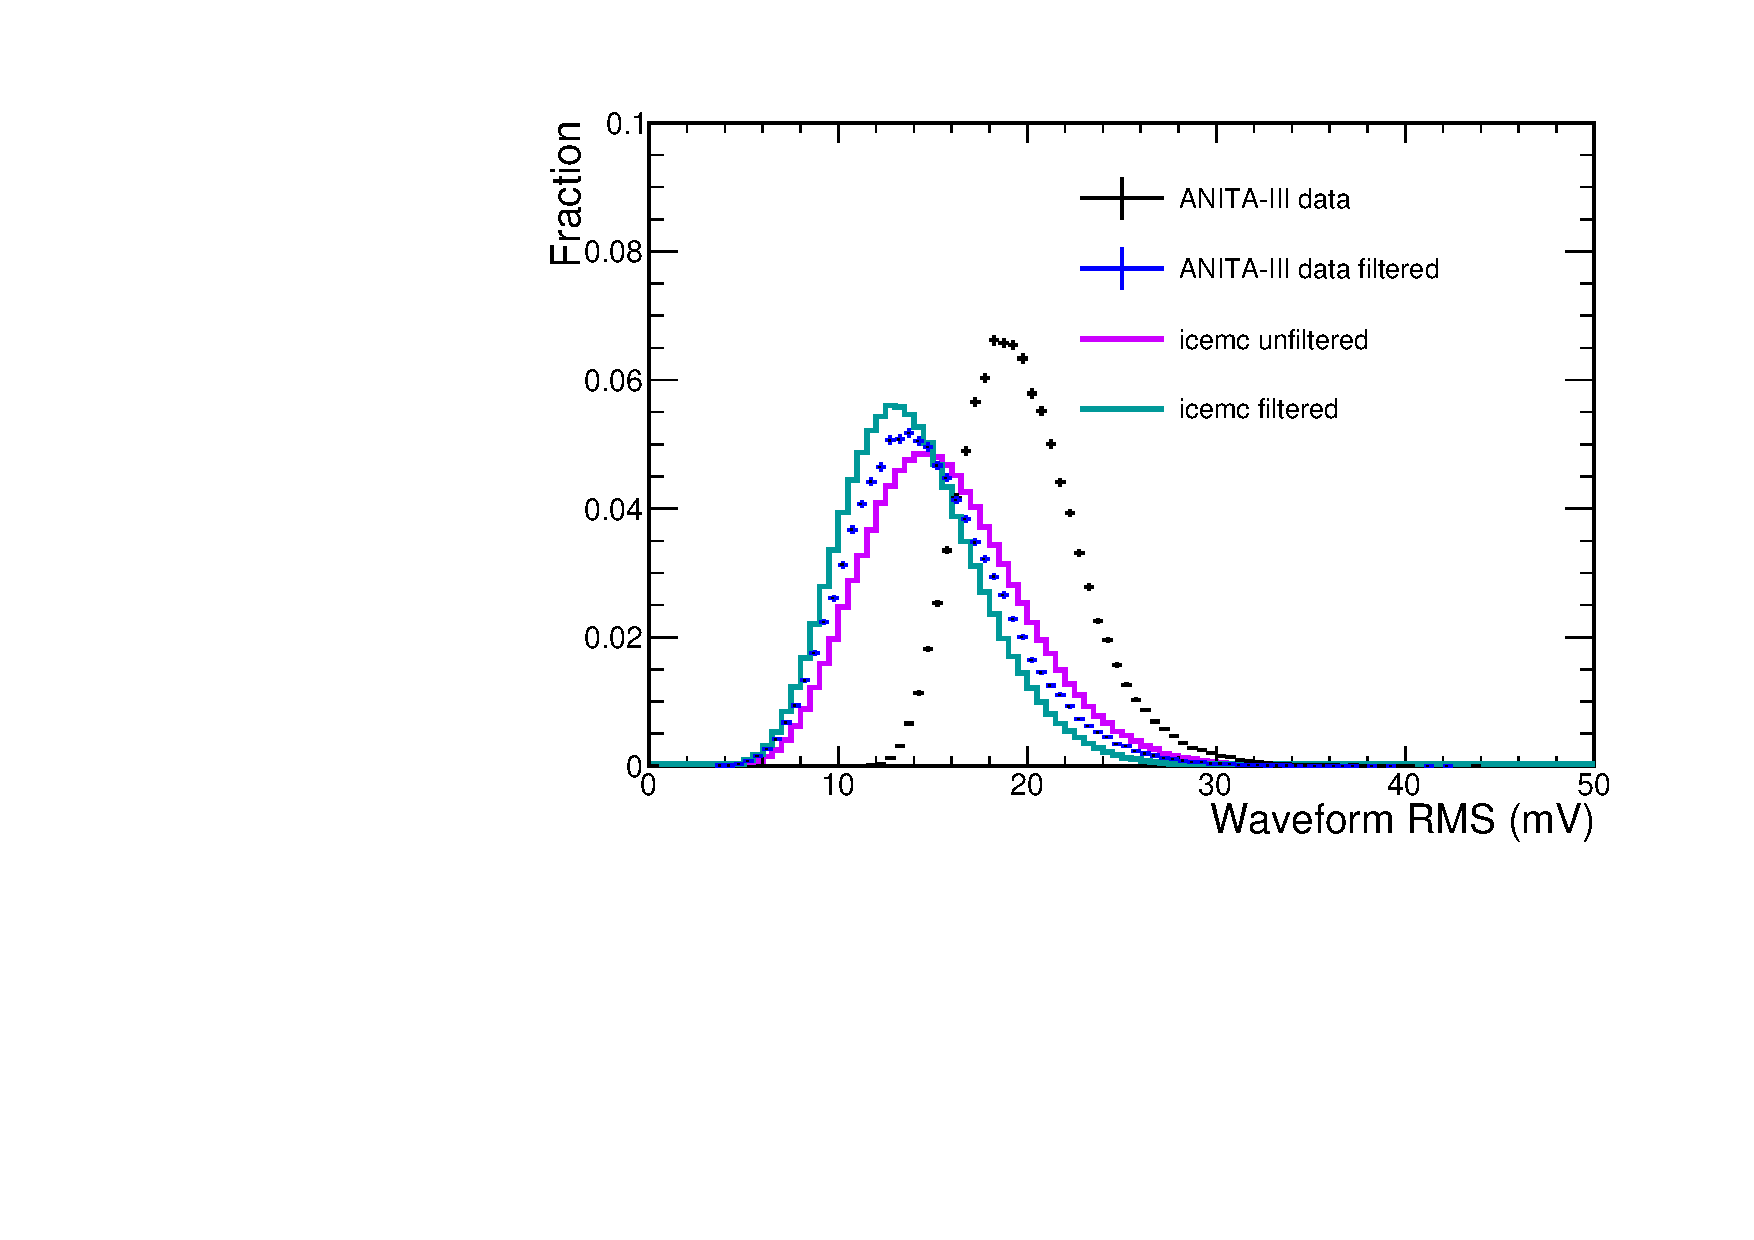
\includegraphics[width=.45\linewidth]{./Figs/ValidationThermalNoiseA3_RMSwaveform.pdf}
  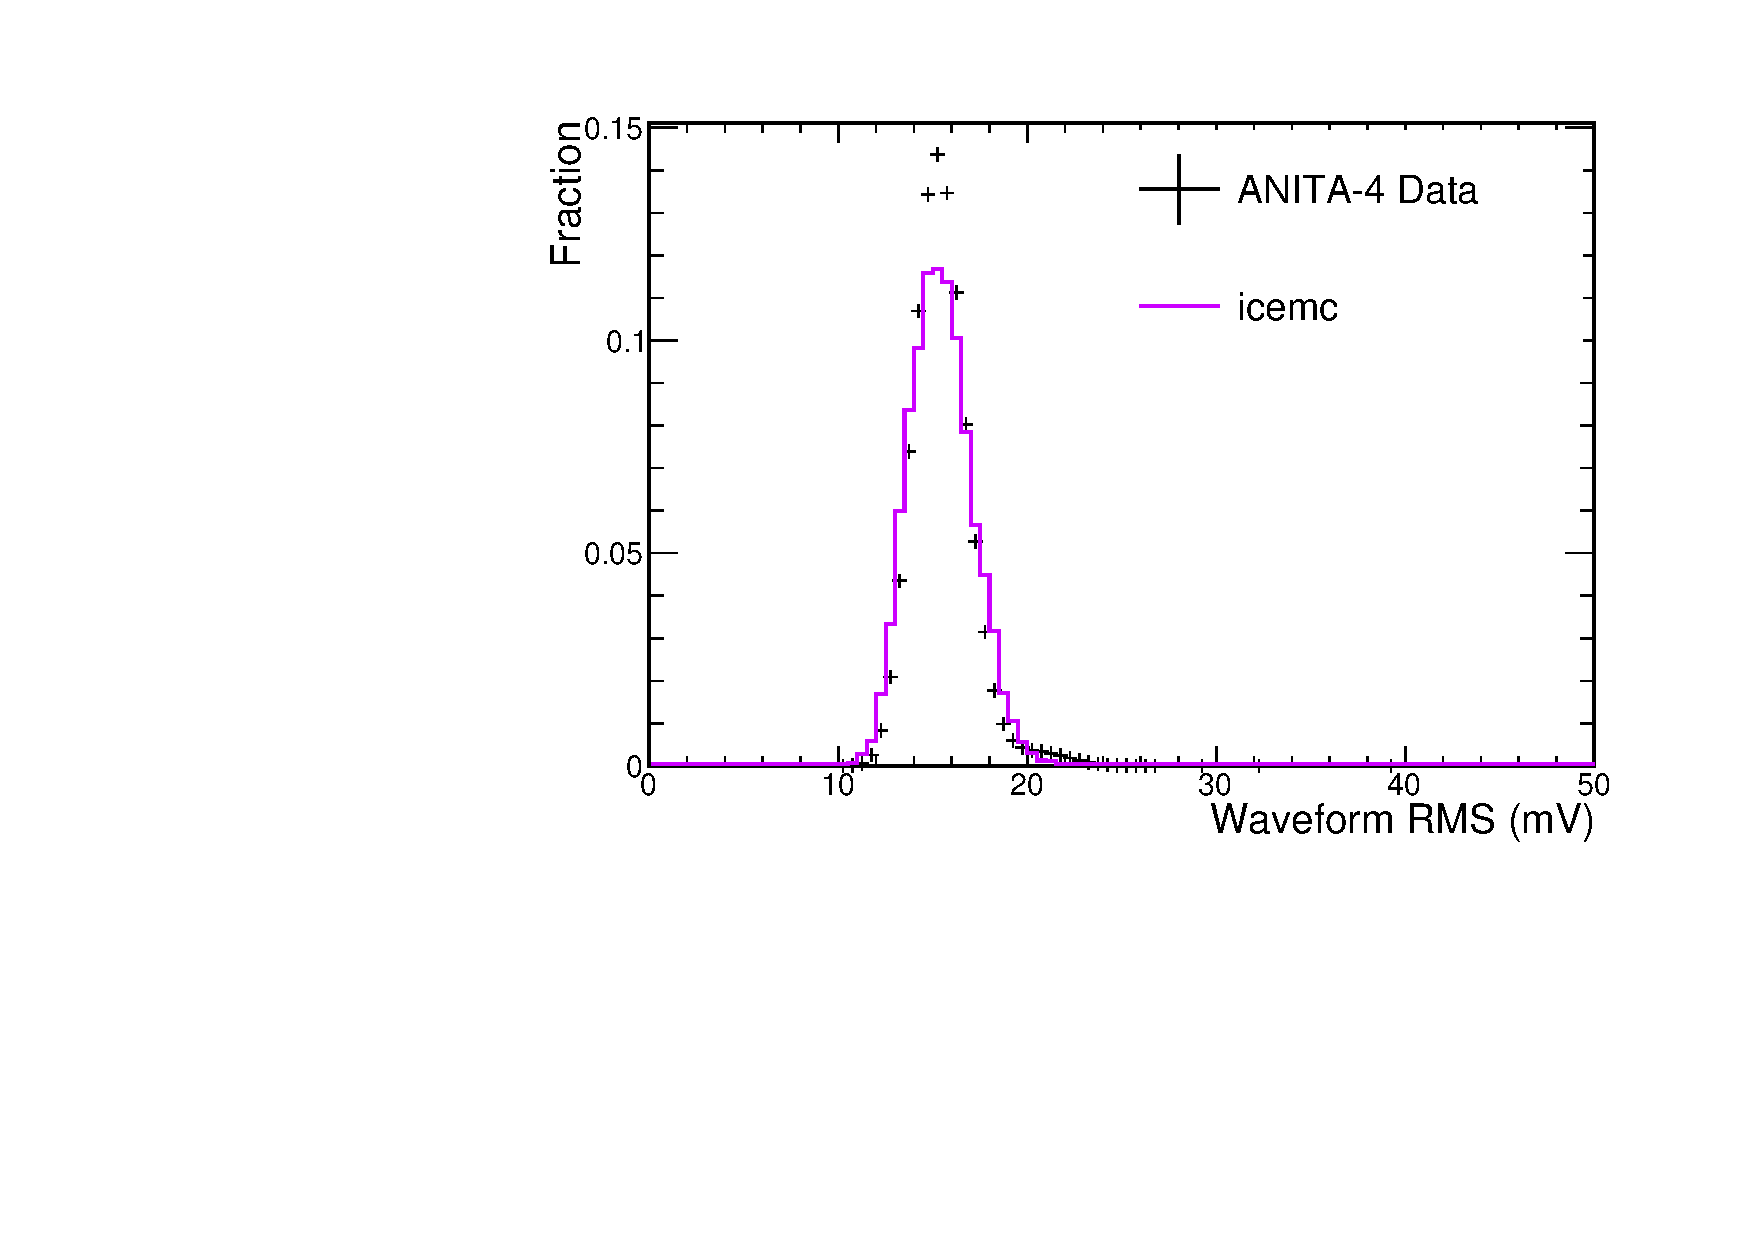
\includegraphics[width=.45\linewidth]{./Figs/ValidationThermalNoiseA4_RMSwaveform.pdf}

\caption{Thermal noise validation. Comparison of RMS of waveforms for an \icemc simulation and a relatively quiet period of the ANITA-III (left) and ANITA-IV (right) flights.
    The ANITA-III flight was affected by strong CW noise that for a better comparison has been filtered out.
    These distributions are area normalized to better compare their shape.
  }
  \label{fig:RMSwaveform}
\end{figure}

As a second self-consistency check, the ANITA-III simulated thermal
noise is also used to produce Rayleigh fits (as described in
Subsection~\ref{subsec:ANITA_thermalNoise}) and shows complete overlap with the fits to the
ANITA-III quiet time.
%Figure~\ref{fig:rayleighGraphs_new} shows that the fits of simulated noise
%completely overlap with the ones coming from the ANITA-III quiet time.

%\begin{figure}[!h]\centering
%  \includegraphics[width=.43\linewidth]{./Figs/RayleighSigma_15H.png}
%  \includegraphics[width=.43\linewidth]{./Figs/RayleighSigma_43H.png}
%  \caption{Thermal noise validation. Graphs of the fitted amplitude ($\sigma(f_i)$) as a
%    function of frequency for channels T15H and B11H (interpolating
%    between filtered frequencies). The new \icemc noise fits
%    completely overlap with the ones coming from the ANITA-III quiet time.}
%  \label{fig:rayleighGraphs_new}
%\end{figure}


\subsubsection{WAIS pulser model}
\label{subsec:wais}
%To aid the validation process, a calibration pulser
%located at West Antarctic Ice Sheet field camp is being added to the simulation

As an additional validation, we model the a calibration pulser located at the West Antarctic Ice Sheet (WAIS) field camp. The WAIS pulser consisted of a 6-kV FID brand pulser that generates a broadband impulse and drives a horizontally polarized antenna. The pulser was triggered on the GPS second with a known delay, permitting a measurement of the  ANITA trigger efficiency while the payload is in view of the pulser.

The antenna used at WAIS, shown and modelled in Fig.~\ref{fig:waisPulser}, is a custom design based on a quad-slot model, for which the slots of the antenna are parallel to the ground. The antenna was installed $\sim$1~m below the surface of the snow. Similar to a discone, the bottom portion of the antenna acts as a reflector, and the angles of the taper on both the reflector and the upper cone tunes the orientation of the peak gain. This design is a scaled down version of the VHF antenna used as a low frequency extension to ANITA-III. The antenna was modelled with the NEC antenna modelling software.

We model the electric field (Figure~\ref{fig:waisPulser}d) generated by the WAIS pulser by convolving the NEC model of the antenna with measurements of the voltage generated by the FID pulser on an oscilloscope.  Fig.~\ref{fig:waisPulser} shows the peak gain for each frequency, the associated phase at that frequency, and the reflection coefficient, $\Gamma$, from the antenna model. The electric field at 1~m from the pulser, $E$, results from relating the power density radiated by the antenna to the power density generated by the pulser with a characteristic impedance $Z_{c}$ and voltage $V$, accounting for loss from imperfect antenna matching between the antenna and the pulser, the magnitude and phase of the gain, $G$, propagation loss, and the impedance of free space, $Z_0$:

\begin{equation}
|E| = \sqrt{\frac{|V|^2}{8 Z_c} (1 -|\Gamma|^2 ) \frac{Z_0}{2\pi (1~\textrm{m})^2} G}
\end{equation}

The electric field shown in Fig.~\ref{fig:waisPulser} is treated as a source in icemc at the location of the WAIS pulser. Figure~\ref{fig:waisEff} shows the efficiency of the ANITA-III payload to generate a trigger from pulses coming from WAIS divide. The simulation efficiency does not asymptote to 1, as it also includes inefficiencies due to the channel masking and the instrument dead time. 
%\CD{And maybe because of the metastability + too-short time windows in A3?} 

\begin{figure}
\centering
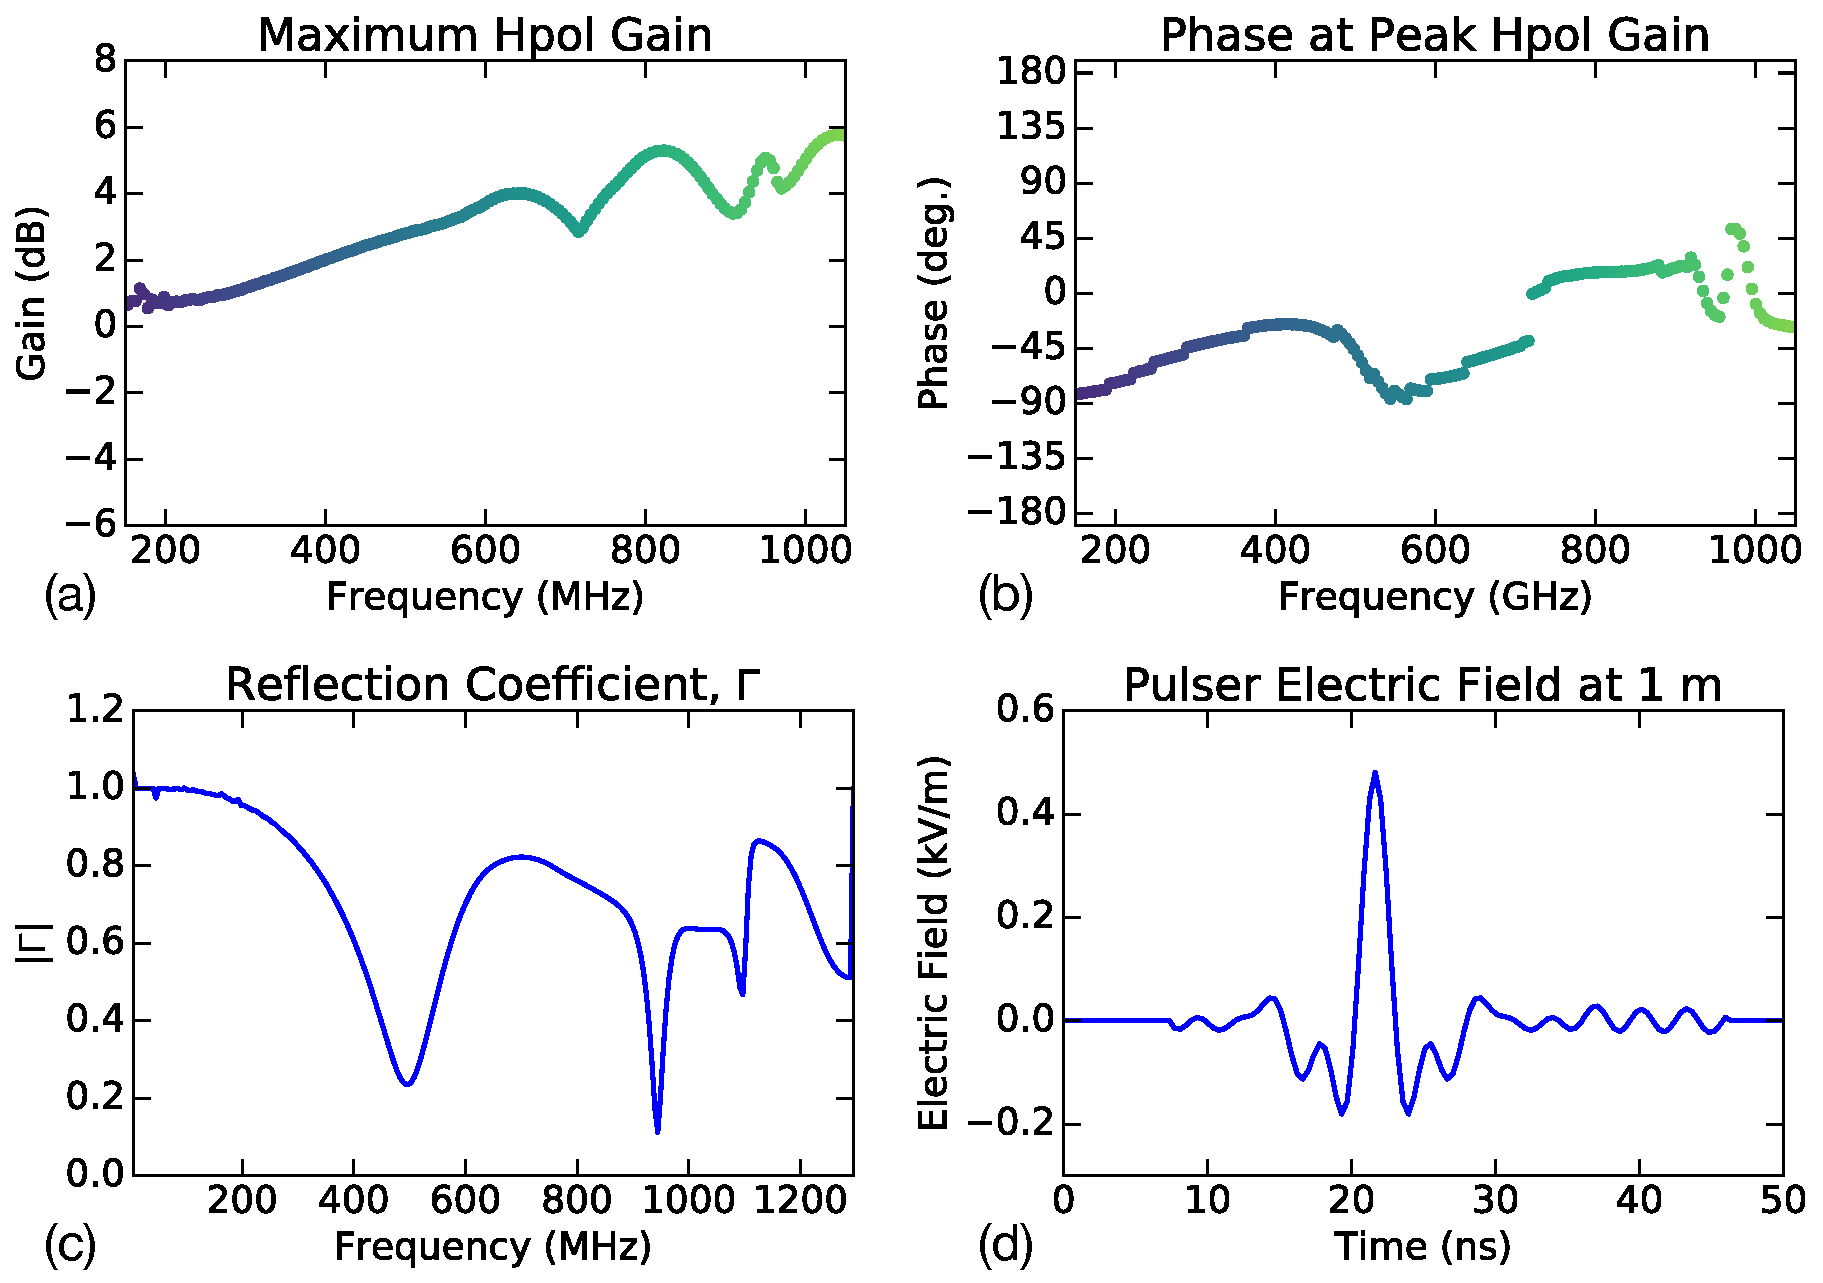
\includegraphics[width=\linewidth]{./Figs/waisPulser.pdf}
\caption{ANITA-III horizontally polarized antenna used in the WAIS pulser}
\label{fig:waisPulser}
\end{figure}

\begin{figure}
\centering
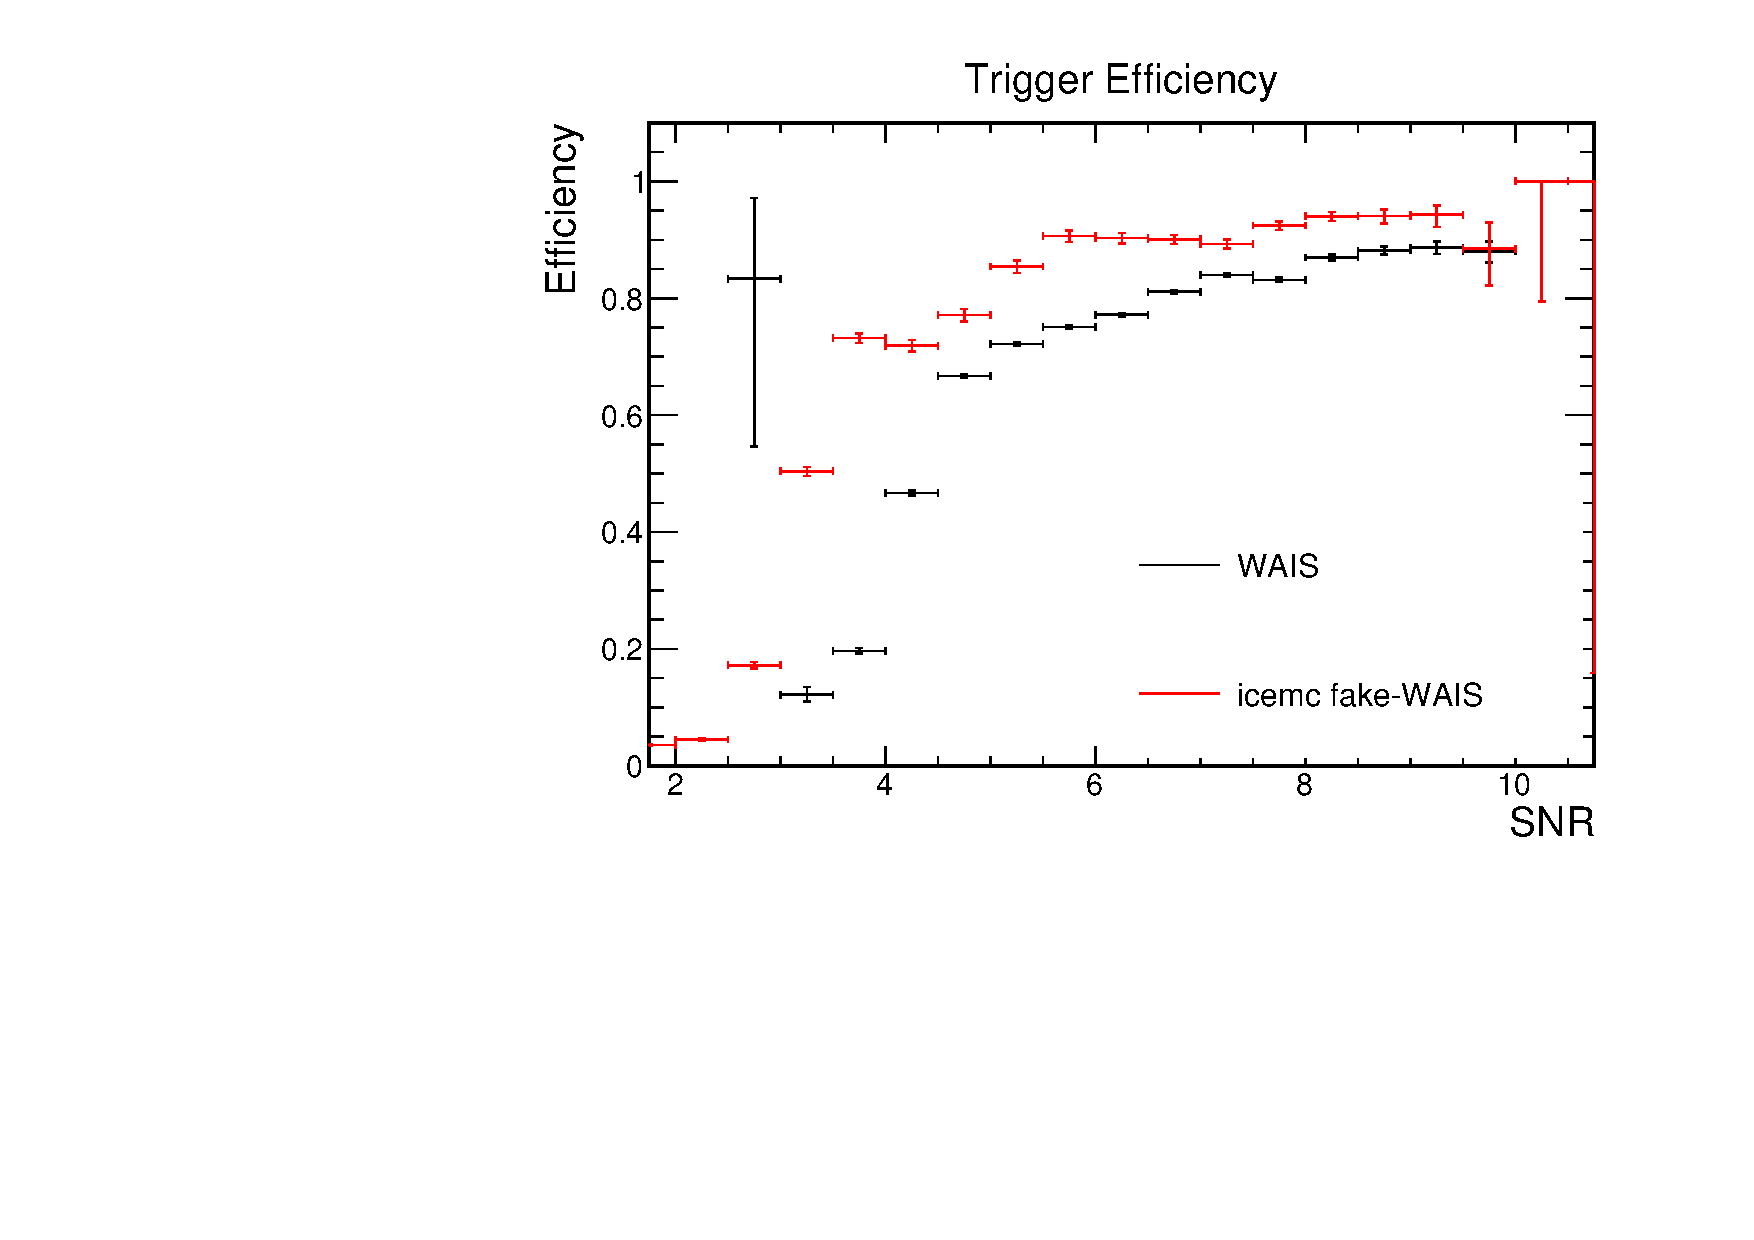
\includegraphics[width=.5\linewidth]{./Figs/Efficiency_WAIS.pdf}
\caption{ANITA-III trigger efficiency to a pulser coming from the WAIS divide station as a function of SNR.}
\label{fig:waisEff}
\end{figure}

\subsubsection{Reconstruction validation}
\label{subsec:ANITA_validation_reconstruction}
To fully validate the simulation, a large sample of simulated
neutrinos is produced following the cosmogenic neutrino flux arising from a mixed cosmic-ray composition as modelled by Kotera et al.~\cite{kotera}.
Simulated waveforms from different triggering channels are
cross-correlated to form a pointing map in the ANITA payload
coordinates, azimuth ($\phi_{meas}$) and elevation
($\theta_{meas}$). 
The peak of the correlation map is then compared to the expected
azimuth ($\phi_{theory}$) and elevation
($\theta_{theory}$), calculated from the true neutrino interaction point.
Details of our reconstruction and analysis can be found in our
previous publications~\cite{ANITA1paper,ANITA2paper,romero2015interferometric}.

%Figure~\ref{fig:pointing} shows the simulation pointing resolution for
%the azimuth and elevation coordinates.
%Both resolutions are compatible with the ANITA-III
%pointing resolution measured using a calibration pulser to be
%0.4\degree in azimuth and 0.2\degree in elevation.


%\begin{figure}[!h]\centering
%  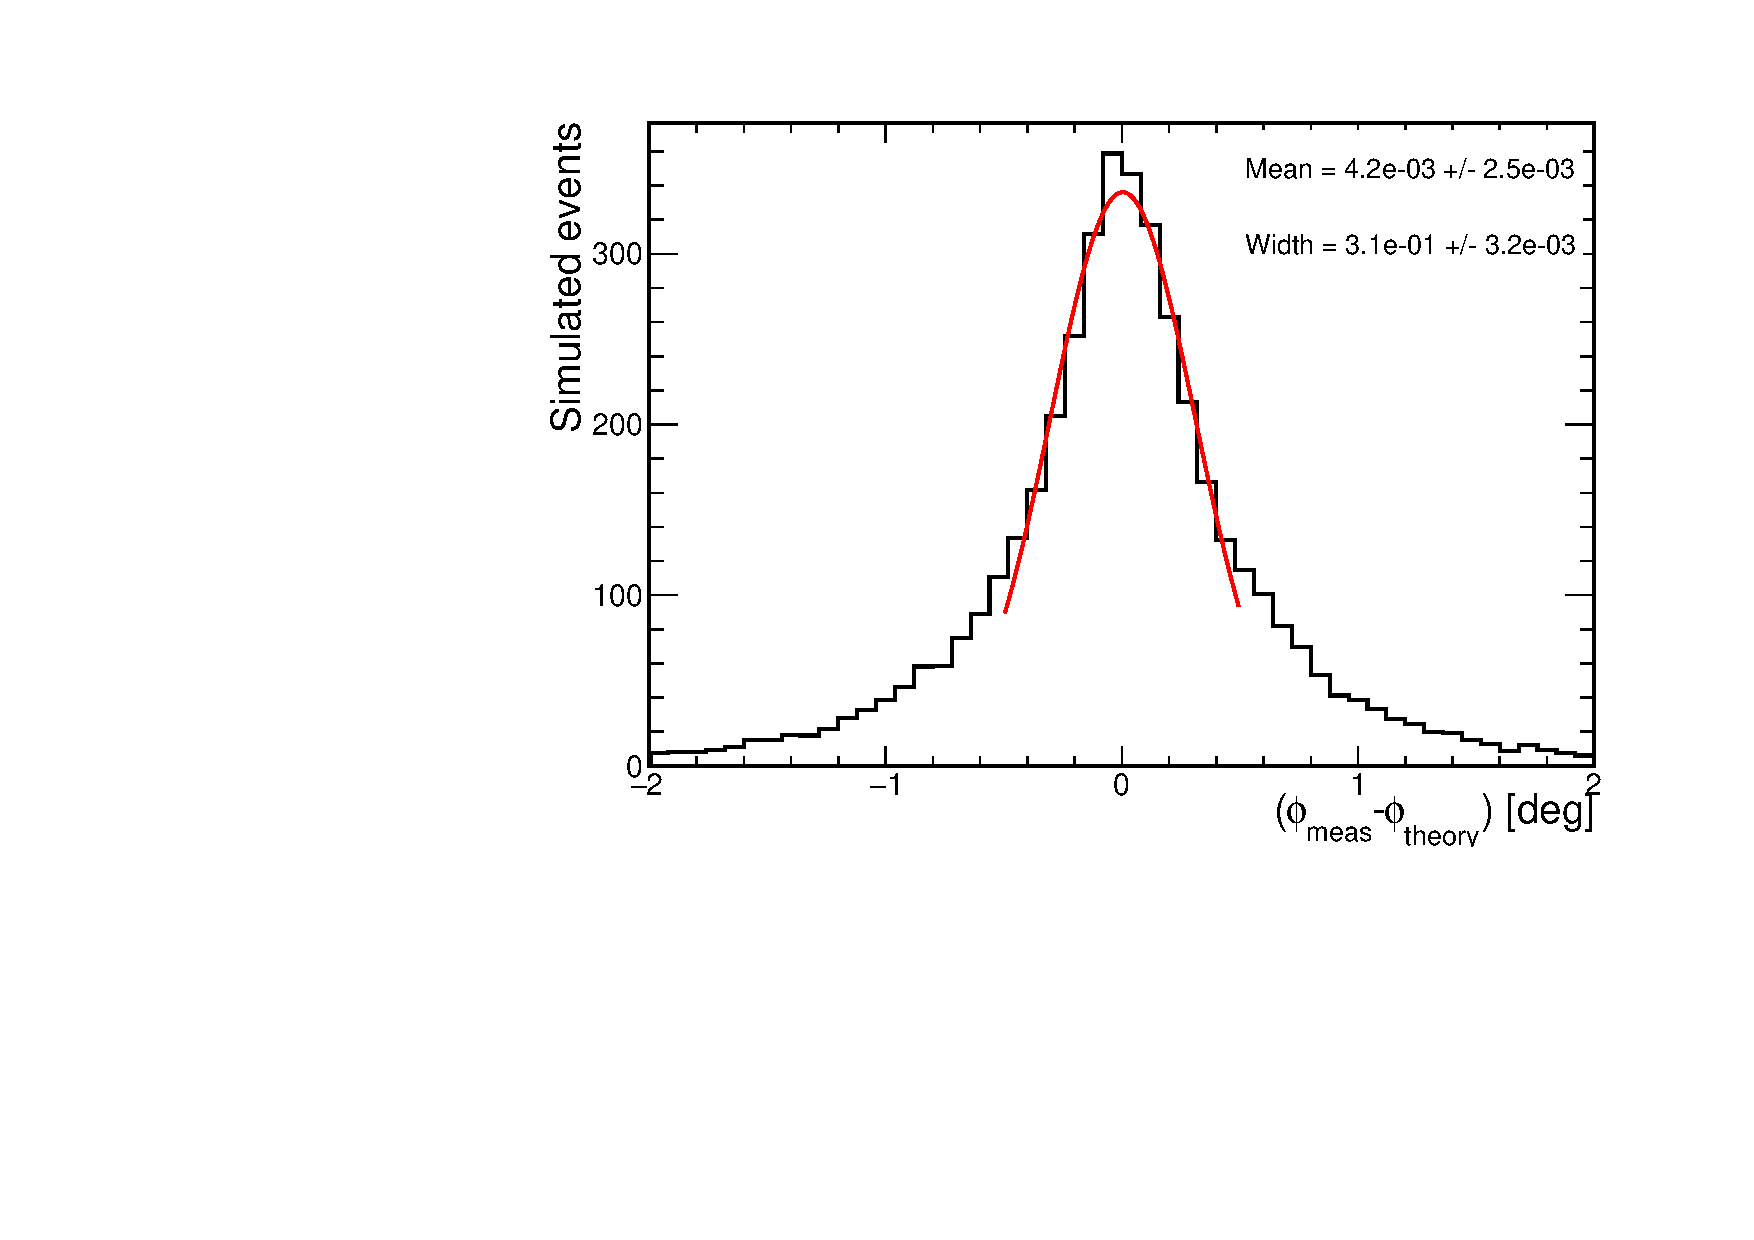
\includegraphics[width=.43\linewidth]{./Figs/KoteraMax_phiresolution.pdf}
%  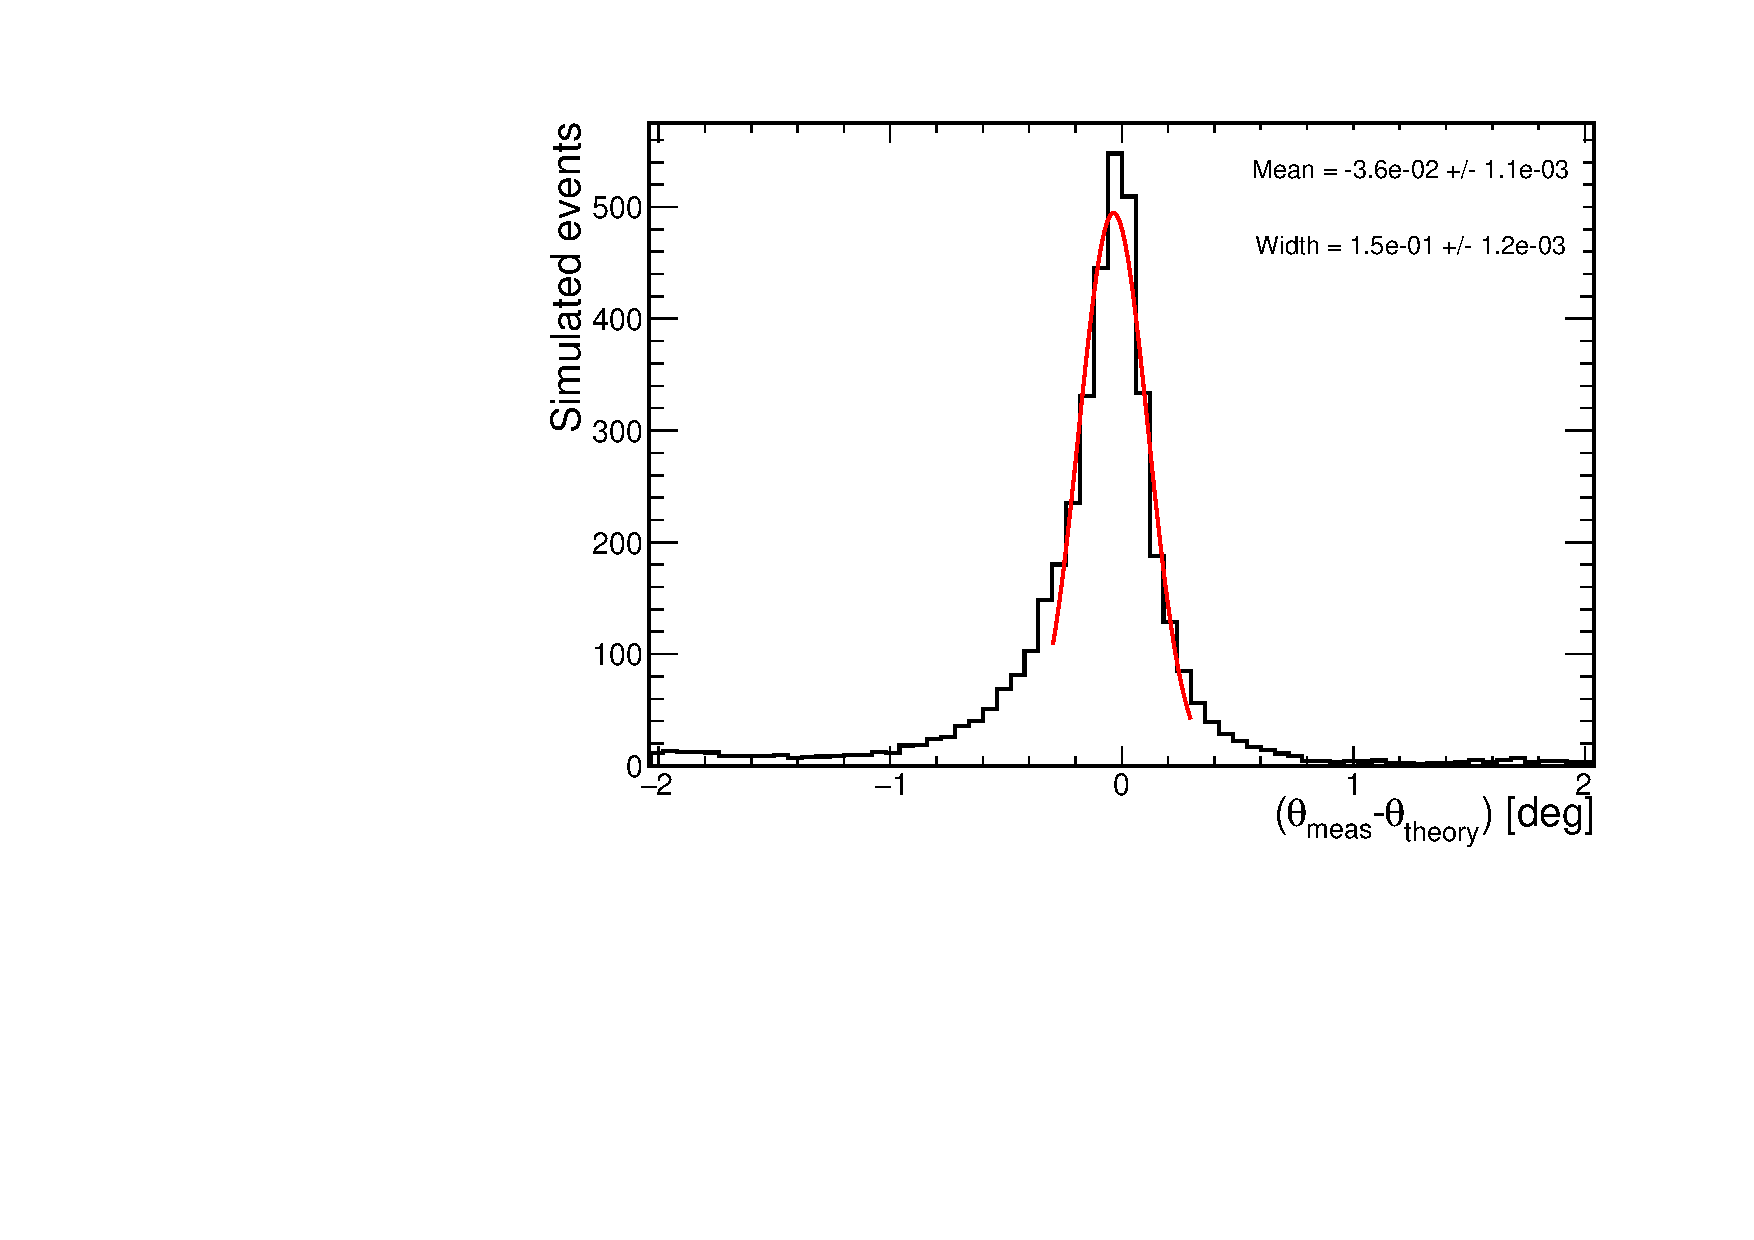
\includegraphics[width=.43\linewidth]{./Figs/KoteraMax_thetaresolution.pdf}
%  \caption{Simulation pointing resolution in azimuth (left) and elevation (right). \CD{The tails don't look very Gaussian here. I think this is because of the quantization of the time intervals. I would leave this out (it doesn't really matter what the pointing resolution is in MC}}
%  \label{fig:pointing}
%\end{figure}


%\subsection{Toy facet model}
%\label{subsec:facet_validation}
%To better understand the effects of surface roughness on the transmitted intensity of the signal, measurements were performed on laser light refracting through ground glass diffusers to determine the transmitted intensity at angles up to and beyond the critical angle~\cite{Griswold:07}.
%The scale of the diffuser surface features compared to the laser wavelength approximately matches the ratio of the dominant Antarctic surface features (sastrugi) to the radio wavelengths sensitive to ANITA.
%Most of the East Antarctic Ice Sheet is characterized by sastrugi with characteristic slopes of about 0.1, corresponding to rms deviations from the surface normal of about 6 degrees \cite{Warren:98}.
%Electron microscope measurements of the diffuser surfaces allow for the determination of their slope distribution, providing a direct comparison to the facet simulations.

%The characteristics rms slope $s_{rms}$ for each diffuser plate is obtained from electron microscope measurements of the local surface heights and features.
%Example images are shown in \cite{Griswold:07}.
%The slope distribution between all points is calculated from the height measurements.
%For self-affine surfaces (surfaces that scale differently in orthogonal directions), the rms slope follows a scaling relationship,
%\begin{equation}
%\label{eqn:affinescaling}
%s(\Delta x) = s_{0}\left( \frac{\Delta x}{\Delta x_{0}} \right)^{H-1},
%\end{equation}
%where $\Delta x$ is stepsize, $\Delta x_{0}$ is the reference stepsize, and $s_{0}$ is the reference slope value for stepsize $\Delta x_{0}$.
%$H$ is the Hurst parameter which describes the slope scaling behavior.
%Additional information can be found in \cite{SHEPARD1999156}.
%For each set of diffuser plate measurements, Eq. \ref{eqn:affinescaling} is fit as a function of the stepsize $\Delta x$ between each set of points, with free parameters $s_{0}$, $\Delta x_{0}$, and $H$.
%This allows for an estimate of the reference slope value $s_{0}$ of the diffuser plate, which is used as input in the facet simulation.

%Figure \ref{fig:facetvalidation} shows a representative comparison of the laser measurement for two different diffuser plates with facet simulation results.
%The thick red dashed line shows the measurement, and the three black thin lines show simulation results for different values of the solid angle subtended by the photosensor.
%The angular extent of the photosensor was about 0.75$^{\circ}$, which is bracketed by the simulation results.
%There is good agreement for all three diffuser plates and across the incidence angle measurements.
%\begin{figure}[!h]\centering
%  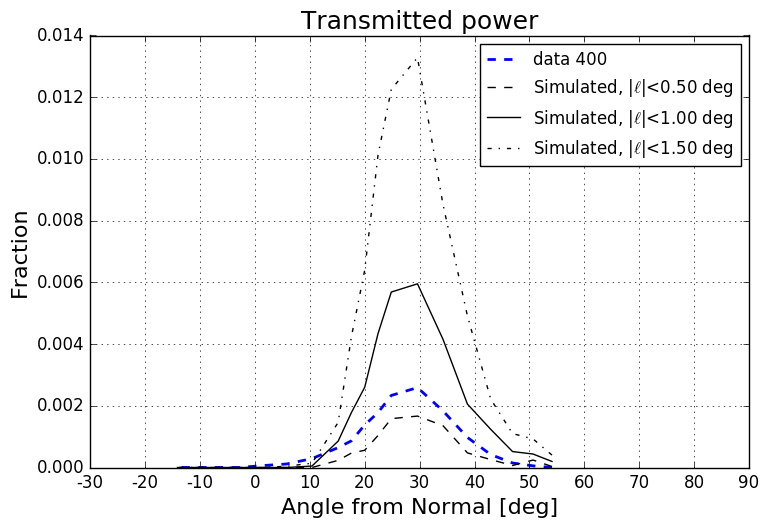
\includegraphics[width=.3\linewidth]{./Figs/reproduce_dist_inc20p0_400.png} %400grit 100um 20deg
%  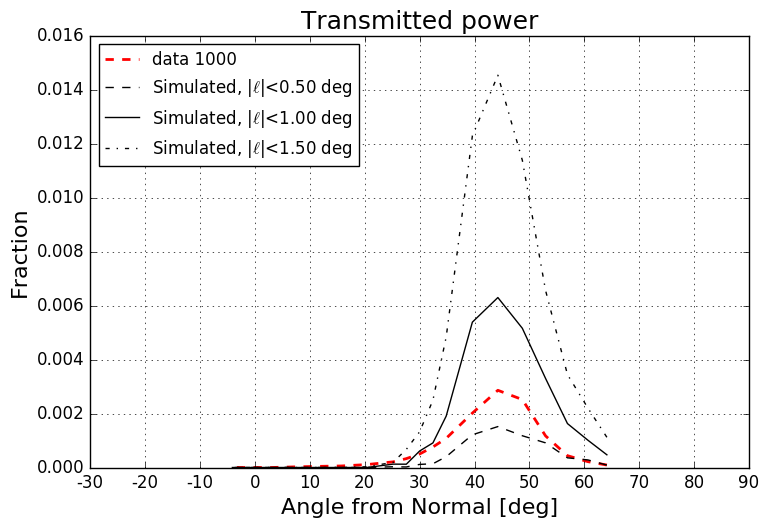
\includegraphics[width=.3\linewidth]{./Figs/reproduce_dist_inc30p0_1000.png} %1000grit 30um 30deg
%  \caption{Facet model validation with laser light measurements.
%  Plots show the fractional transmitted power as a function of the angle away from the surface normal for two of the diffuser plates.
%  Angles larger than 90 degrees lie parallel to the direction of the incident ray.}
%  \label{fig:facetvalidation}
%\end{figure}


\section{ANITA sensitivity}
\label{sec:results}

The simulation files produced with \icemc are used by the ANITA analysts to tune analysis cuts, check the rate of accidental clustering, and also to simulate sources like Gamma Ray Bursts and Active Galactic Nuclei.
Finally, the simulation is used to calculate the experiment sensitivity.

\subsection{Acceptance}
\label{subsec:acceptance}
The ANITA collaboration uses \icemc to calculate the experiment volumetric acceptance \effvol, following:
\begin{equation}
  \label{eq:volacceptance}
  \effvol = \dfrac{n_{{pass}}(E)V_0\Omega}{N(E)} \;,
\end{equation}
\noindent where
 $n_{{pass}}(E)$ is the weighted (see Section~\ref{sec:weights}) number of events that pass the trigger at a given energy $E$,
 $V_0$ is the volume of ice in Antarctica viewed by ANITA,
$\Omega$ is $4\pi$ steradians, and 
 $N(E)$ is the number of neutrino events thrown by each simulation at that energy $E$.

The ANITA acceptance (\effarea) is calculated following:
\begin{equation}
  \label{eq:acceptance}
  \effarea = \dfrac{\effvol}{\ell_{{int}}(E)} \;,
\end{equation}
\noindent where
 \effvol is the volumetric acceptance and
 $\ell_{{int}}(E)$ is the average interaction length in that energy bin. 
The interaction length is calculated following:
 \begin{equation}
   \label{eq:intlength}
    \ell_{{int}}(E_\nu) =   \dfrac{M_{NUCL}}{\sigma(E) \rho_{H_2O} } \;,
  \end{equation}
  
\noindent where
 $M_{NUCL}$ is the atomic nuclear mass ($1.66\cdot 10^{-27}$\,kg),
 $\rho_{H_2O}$ is the density of water (1000\,kg/m$^3$), 
and $\sigma(E)$ is the neutrino cross-section for $\nu$ charged-current interactions.
Currently the neutrino cross-section is calculated using either the
Reno {\it et al.}~\cite{reno2005high}
or the Connolly {\it et al.}~\cite{PhysRevD.83.113009} parametrizations.
The latter is the default.

Although recent neutrino cross-section measurements by the IceCube
Collaboration reached the multi-TeV
scale~\cite{aartsen2017measurement,bustamante2017measurement}, 
above this energy there are
only cross section measurements with an uncertainty of a factor $\pm 5$ up to
300\,TeV.
The current theoretical models can extrapolate the cross-sections up to $10^{21}$\ev~\cite{PhysRevD.83.113009,reno2005high},
but the associated uncertainties are
large, and the impact on the ANITA acceptance is
non-negligible.
Figure~\ref{fig:acceptanceVSxsec}~(left) shows the effect of changing the
cross-section parametrization on the ANITA-III acceptance.
The nominal Connolly {\it et al.} parametrization is compared to the upper and lower bound set by
Reference~\cite{PhysRevD.83.113009}, and to the alternate
parametrization suggested by Reference~\cite{reno2005high}.


\begin{figure}[!h]\centering
  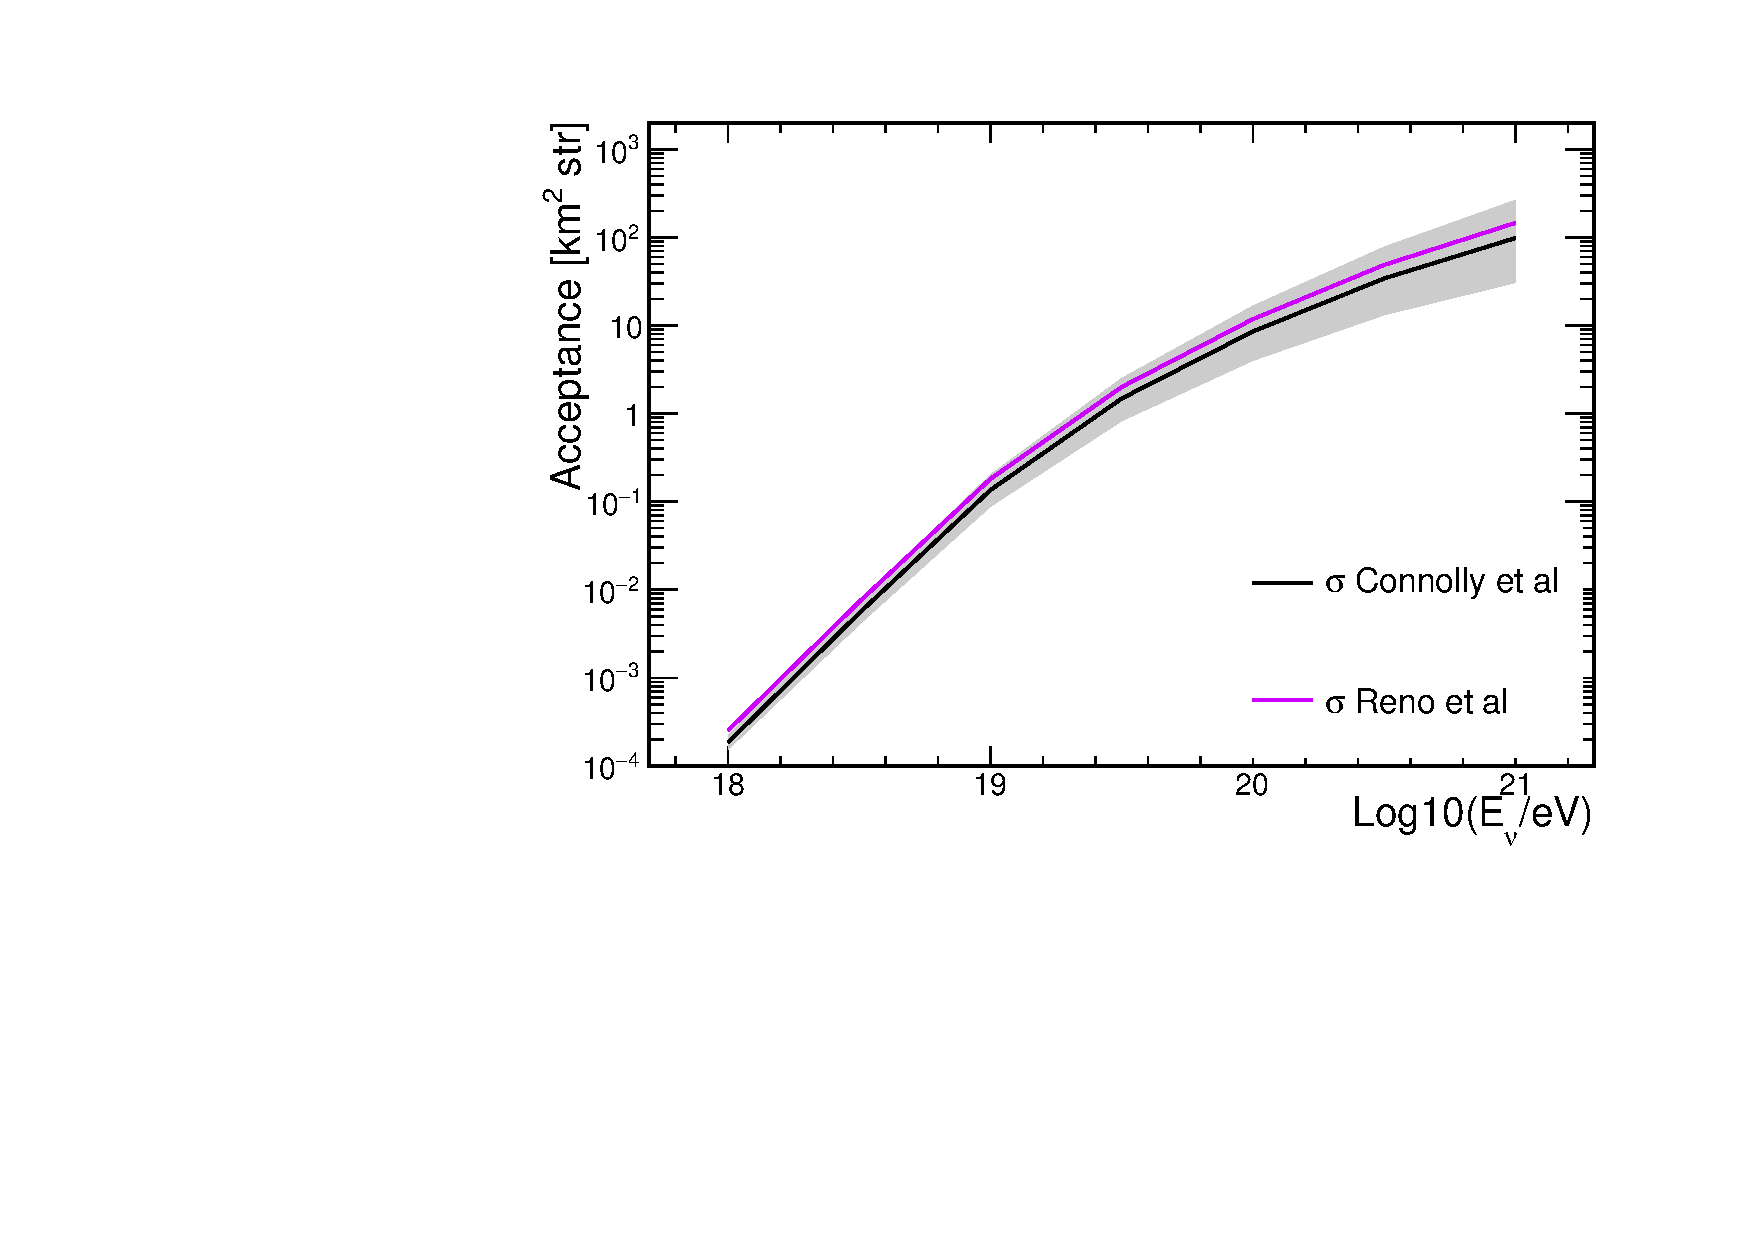
\includegraphics[width=.45\linewidth]{./Figs/AcceptanceVScrossSectionParam_ANITA3.pdf}
  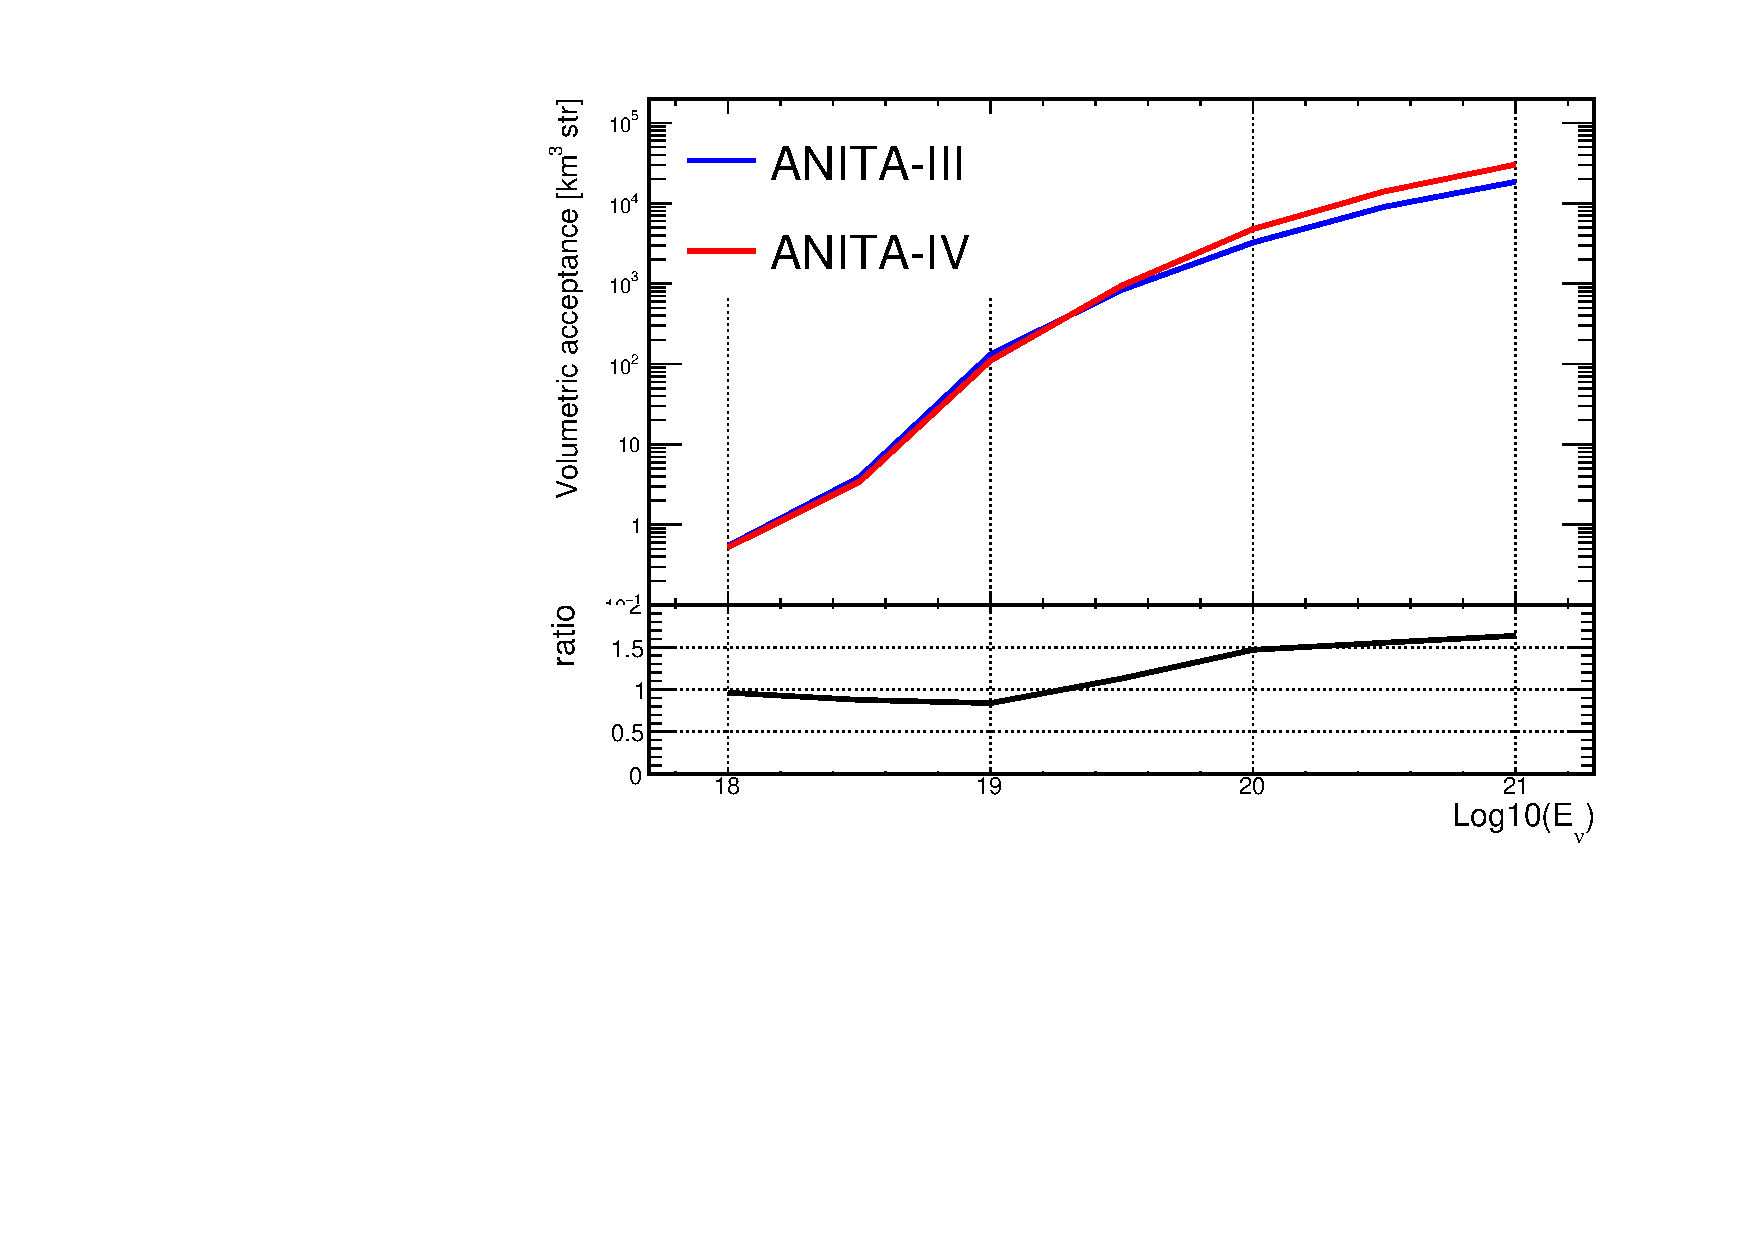
\includegraphics[width=.45\linewidth]{./Figs/CompareEffVol_A3vsA4.pdf}
  \caption{(Left) ANITA-III acceptance for different cross-section parametrizations: Connolly et al.~\cite{PhysRevD.83.113009} and Reno et al.~\cite{reno2005high}. (Right) ANITA-III and ANITA-IV volumetric acceptance comparison as a function of energy.}
  \label{fig:acceptanceVSxsec}
\end{figure}


\begin{figure}[!h]\centering
  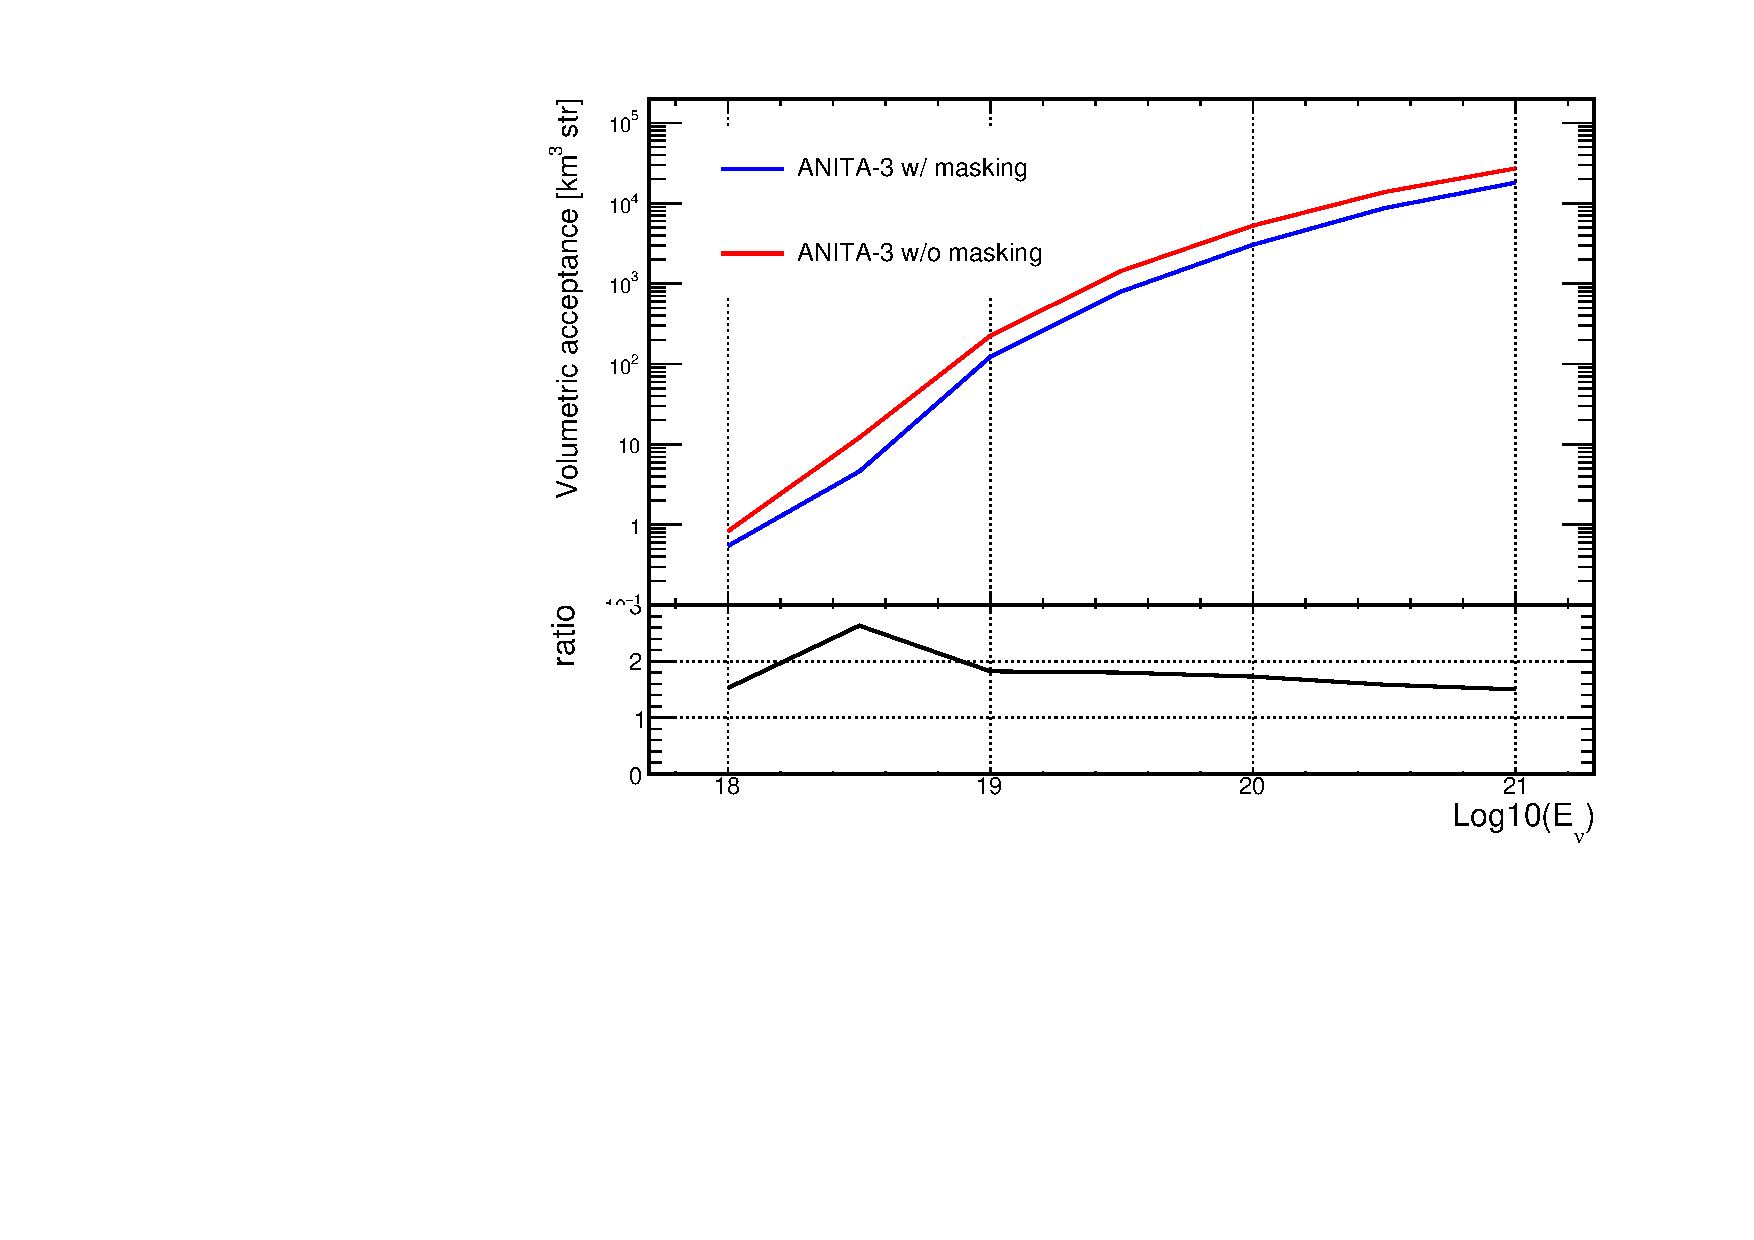
\includegraphics[width=.45\linewidth]{./Figs/CompareEffVol_A3masking.pdf}
  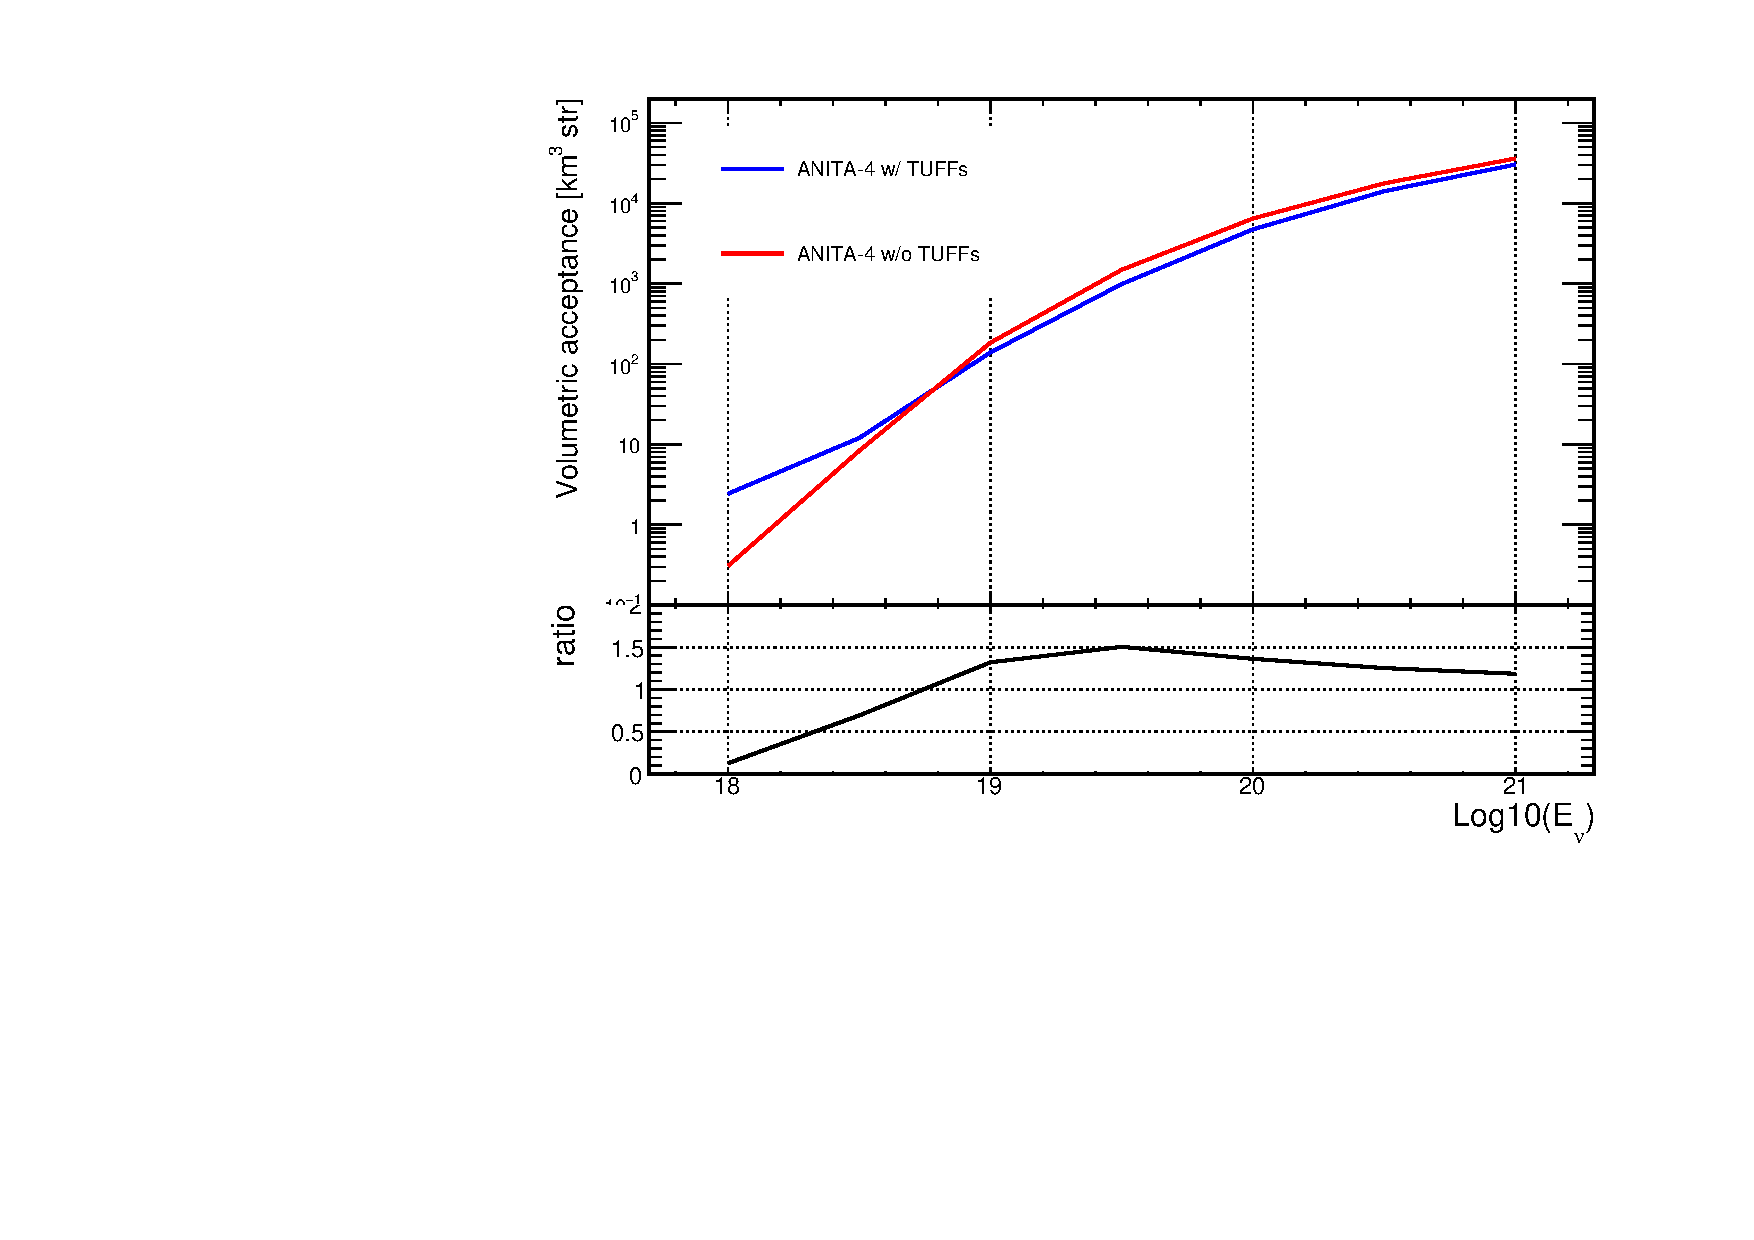
\includegraphics[width=.45\linewidth]{./Figs/CompareEffVol_A4tuff.pdf}
  \caption{(Left) Comparison of ANITA-III volumetric acceptance with and without channel masking.
  (Right) Comparison of ANITA-IV volumetric acceptance with and without TUFFs.}
  \label{fig:acceptanceVariations}
\end{figure}

Figure~\ref{fig:acceptanceVSxsec}(right) shows the ANITA-III and ANITA-IV volumetric acceptances and their ratio.
The ANITA-IV hardware improvements (use of better low noise
amplifiers, the tunable notch filters to avoid carrier wave noise, and
the use of LCP-RCP trigger coincidences to avoid satellite noise) 
enabled ANITA-IV to increase the volumetric acceptance by 50\% at the
highest energy.

Volumetric acceptances are also used to compare the impact of different hardware choices.
ANITA-III was highly affected by satellite noise and had to employ channel masking throughout the entire flight to avoid overloading the trigger. Figure~\ref{fig:acceptanceVariations}~(left) shows that channel masking reduced the ANITA-III sensitivity by more than 50\% across all energy bins.
ANITA-IV used the TUFF boards to avoid carrier wave noise: Figure~\ref{fig:acceptanceVariations}~(right) shows the impact of the tunable filters on the ANITA-IV sensitivity which was reduced by 25--50\%.

Figure~\ref{fig:moreAcceptanceVariations} shows the variation of the ANITA-IV volumetric acceptances coming from different \icemc parameter variations.
The black solid line shows the effect of using BEDMAP instead of CRUST 2.0 as Antarctica ice model; the more finely binned BEDMAP map results in a roughly 20\% lower acceptance over all energies.
The orange solid lines shows the effect of varying the random surface inclination, the two cases shown are 0 and 2.4\%, where the latter is double the nominal value.
The violet area shows the effect of using constant trigger thresholds instead of time varying thresholds; the violet area is the result of using the minimum and maximum thresholds for the whole flight.

\begin{figure}[!h]\centering
  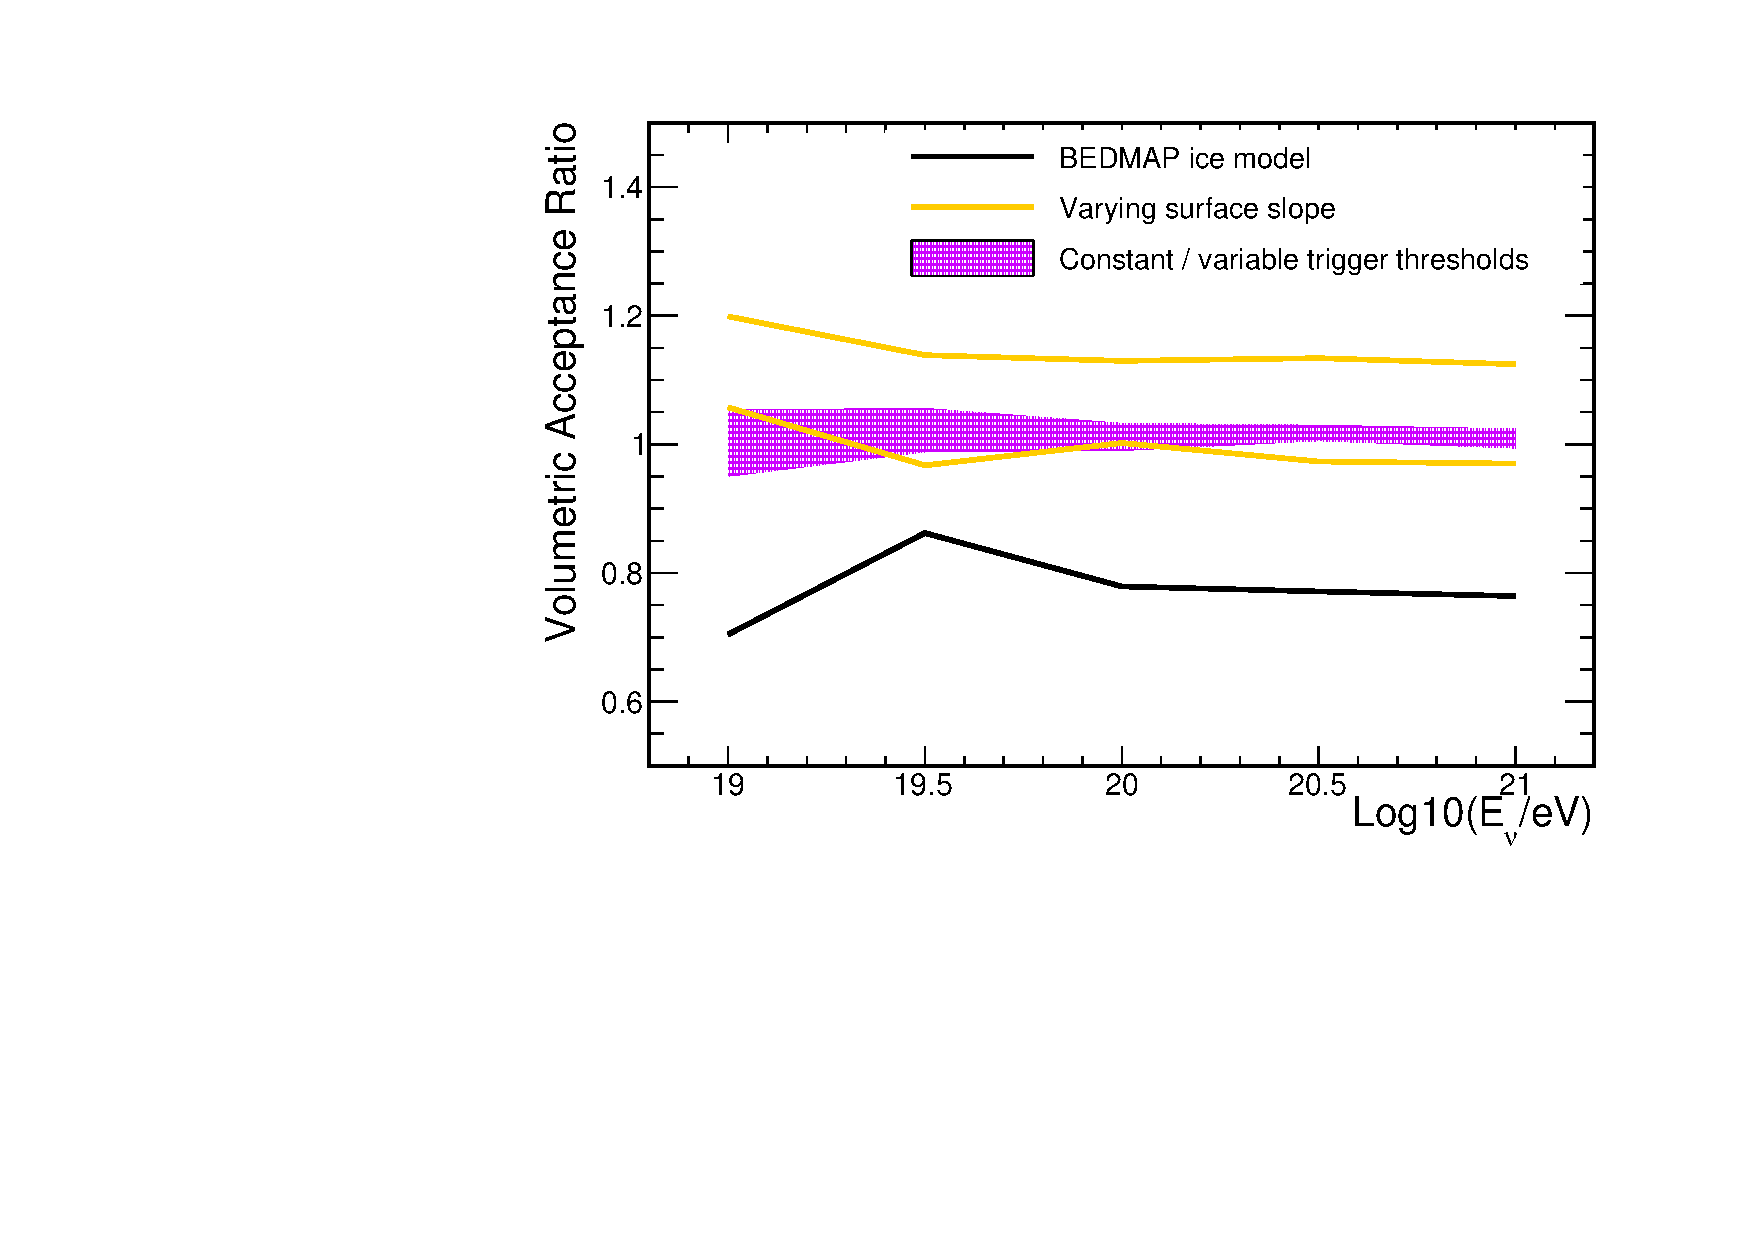
\includegraphics[width=.45\linewidth]{./Figs/SystUncertaintiesForPaper.pdf}
  \caption{Ratio of ANITA-IV volumetric acceptances as a function of energy found varying different \icemc parameters. The solid black line shows the variation coming from using BEDMAP instead of CRUST 2.0 as Antarctica ice model.
  The orange solid lines are calculated by setting the surface slope inclination at 0 or 2.4\% (double the nominal).
  The violet area is found by using constant trigger thresholds instead of time varying thresholds. }
  \label{fig:moreAcceptanceVariations}
\end{figure}

\subsection{Limit}
\label{subsec:limit}
The projected 90\% confidence level on the diffuse neutrino flux is set by using:
\begin{equation}
\left( \dfrac{Ed^4N}{dE dA d\Omega dt}\right)_{lim} =
\dfrac{s_{up}}{ T \cdot \epsilon_{ana} (E_\nu) \cdot \effarea \cdot \Delta} \, ,
\end{equation}
\noindent
where
$s_{up}$ is the upper (one-sided) limit for the mean of a Poisson
variable given 0 observed events in the absence of background for 90\%
CL, 
$T$ is the live time 
(17.4 days for ANITA-III and 24.25 days for ANITA-IV), 
$\epsilon_{ana}(E_\nu)$ is the neutrino analysis efficiency,
\effarea is the experiment acceptance as a function of the neutrino
energy, and $\Delta=4$ is a model-independent factor following Reference~\cite{PhysRevD.73.082002}.


Figure~\ref{fig:sensitivity} shows the ANITA-III, ANITA-IV and ANITA\,I-IV limits as calculated in References~\cite{anita3cosmogenic,anita4cosmogenic}.
These are compared to the latest constraints coming from the IceCube~\cite{icecube2018} and Auger experiments~\cite{auger2017}, as well as
four cosmogenic neutrino models~\cite{kkss2002,takami2009,ahlers2012,kotera2010cosmogenic}.

\begin{figure}[!h]\centering
 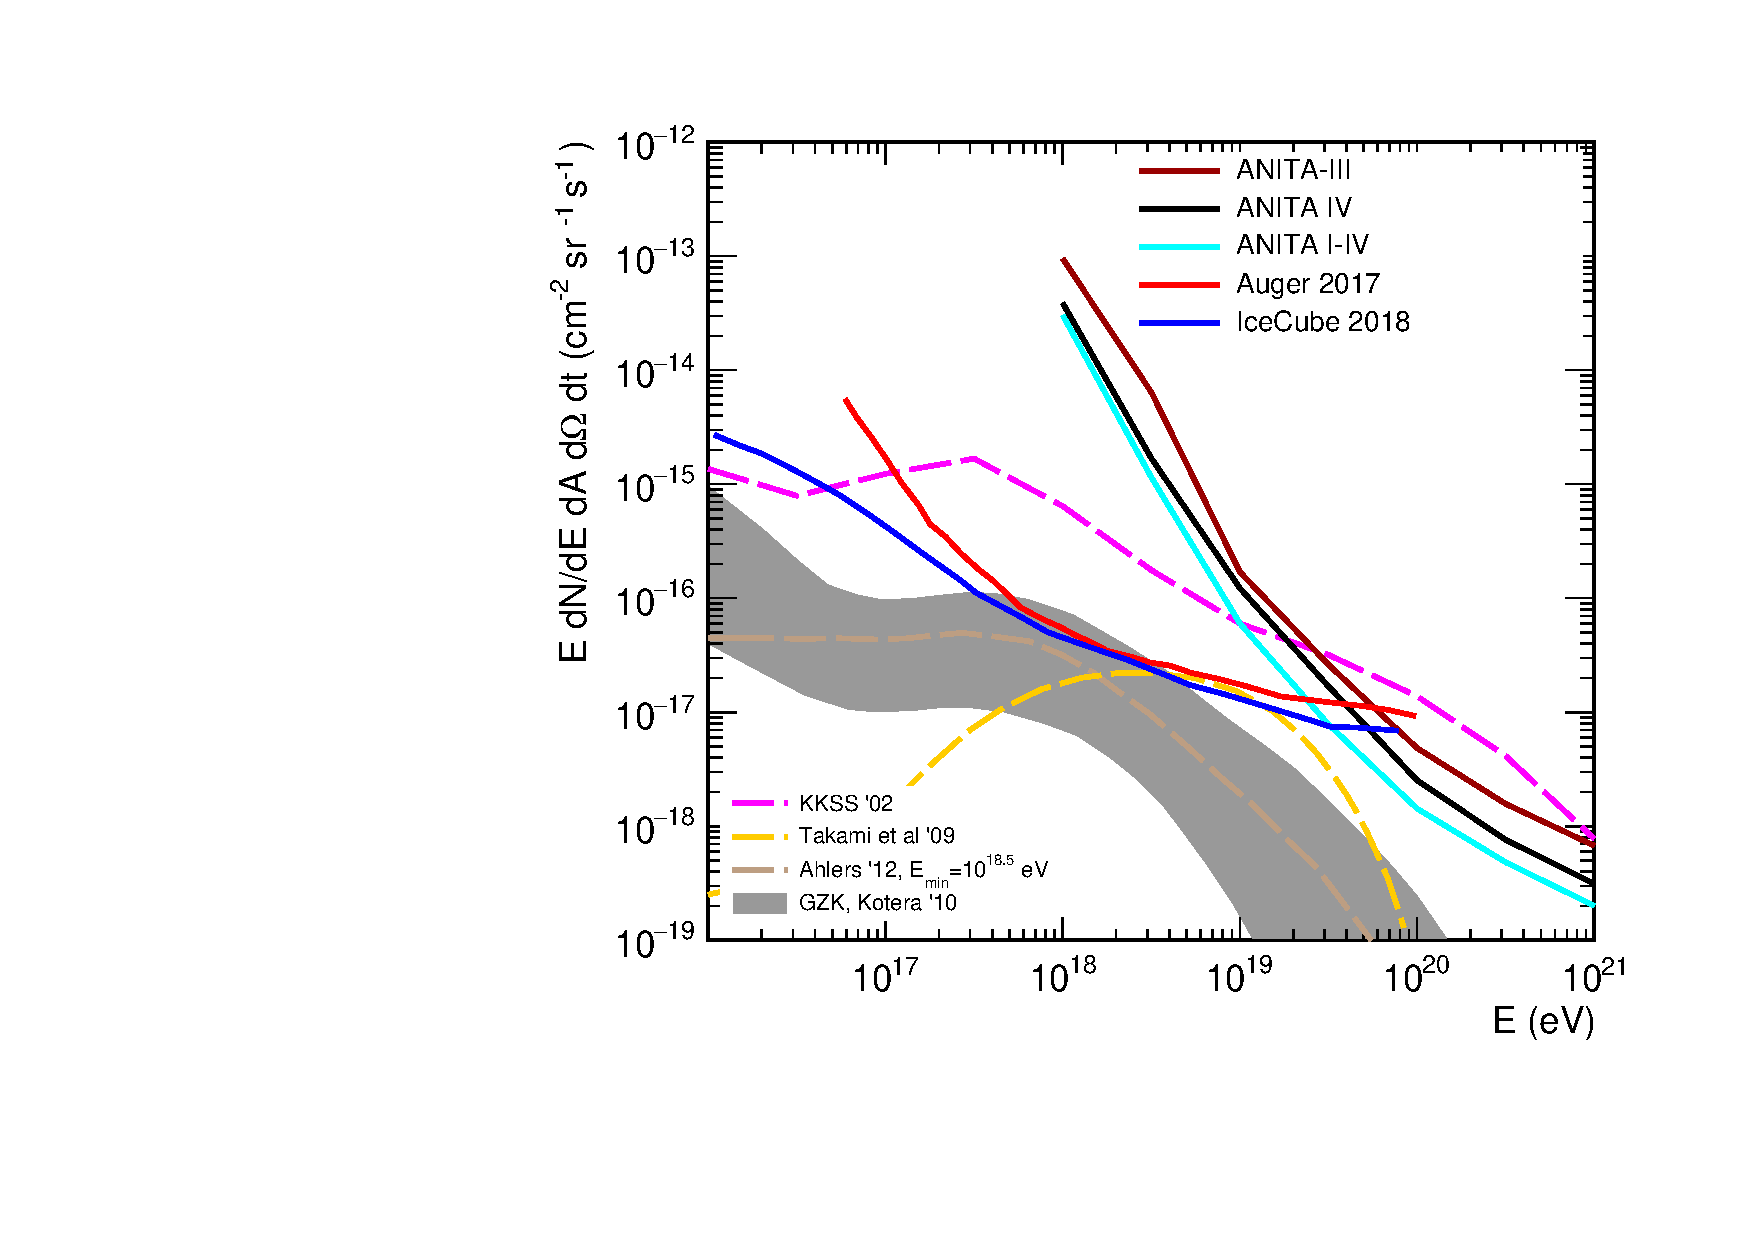
\includegraphics[width=.65\linewidth]{./Figs/Limit4icemcPaper.pdf}
 \caption{
 ANITA-III and ANITA-IV limit on the all flavor diffuse UHE neutrino flux and a combined limit from ANITA I-IV, as calculated in References~\cite{anita3cosmogenic,anita4cosmogenic}.
 The most recent UHE neutrino limits
from the Auger~\cite{auger2017} and IceCube~\cite{icecube2018} experiments, and
four cosmogenic neutrino models~\cite{kkss2002,takami2009,ahlers2012,kotera2010cosmogenic} are also displayed. 
}
 \label{fig:sensitivity}
\end{figure}

\section{Summary and Future improvements}
\label{sec:future}
The \icemc Monte Carlo simulation program is used for the
simulation of ultra high energy neutrino interactions in the Antarctic
ice and their detection by the ANITA experiment.
The data taken before or during the ANITA flights are used to validate the
simulation.
The latest ANITA-III, ANITA-IV and ANITA\,I-IV performance is provided in the form of the
acceptance and energy dependent neutrino limit.
 
Future versions of the program will include the possibility to use extensive air showers inputs from ZHAireS~\cite{alvarez2012monte}; improved and refined ice properties modeling and surface roughness effects; the contribution of the sun to the thermal noise; and carrier wave noise as measured during the ANITA-III and ANITA-IV flights.
We are also working towards expanding the framework so that it can be used by multiple radio experiments based in Antarctica.


\section{Acknowledgements}
\label{sec:ackowledgements}
We would like to thank the National Aeronautics and Space Administration and the National Science Foundation.  We would especially like to thank the staff of the Columbia Scientific Balloon Facility and the logistical support staff enabling us to perform our work in Antarctica.  We are deeply indebted to those who dedicate their
careers to help make our science possible in such remote environments.
This work was supported by the Kavli Institute for Cosmological Physics at the University of Chicago.  Computing resources were provided by the University of Chicago Research Computing Center and the Ohio Supercomputing Center at The Ohio State University.
A. Connolly would like to thank the National Science Foundation
for their support through CAREER award 1255557. 
O. Banerjee and L. Cremonesi's work was also
supported by collaborative visits funded by the Cosmology and Astroparticle
Student and Postdoc Exchange Network (CASPEN).
The University College London group was also supported by the Leverhulme Trust. The Taiwan team is supported by Taiwan's Ministry of Science and Technology (MOST) under its Vanguard Program 106-2119-M-002-011.

\bibliographystyle{Styles/JHEP}
\renewcommand{\bibname}{References}
\bibliography{references.bib} 

\appendix

\section{Obtaining and using \icemc}
\icemc can be obtained from the GitHub repository \url{https://github.com/anitaNeutrino/icemc}.
The only mandatory requirement for the compilation of \icemc is a ROOT~\cite{brun1997root} installation.
The compilation can be executed via the Makefile or using the CMake structure.

To run \icemc one needs to define two environment variables and add them to the global path:
\begin{itemize}
    \item  \texttt{ICEMC\_SRC\_DIR} should point to the directory where the source code is saved;
    \item  \texttt{ICEMC\_BUILD\_DIR} should point to the directory where the executable programs are.
\end{itemize}

To run icemc one can simply do:
\begin{verbatim}
./icemc -i {inputFile} -o {outputDirectory} -r {runNumber}
-n {numberOfNeutrinos} -t {triggerThreshold} -e {energyExponent}
\end{verbatim}

All of the parameters are optional and if they are not specified inputs from \texttt{inputs.conf} are used. 
The two standard input files for the ANITA-III and ANITA-IV flights come with the package.

The output directory contains a series of root files with  information about all the neutrinos simulated, as well as a text file containing the neutrino survival efficiency at different stages of \icemc, and the volumetric acceptance.

Other programs test a portion of the full \icemc tool:
\begin{itemize}
    \item {\tt testThermalNoise} simulates only the thermal noise at the payload for a specific ANITA flight.
    \item {\tt testInputAfterAntenna} simulates the injection of an RF impulse after the antenna feed; this program is used to produce trigger efficiency scans similar to the ones taken before each ANITA flight.
    \item {\tt testWAIS} simulates the WAIS pulser as described in Subsection~\ref{subsec:wais}.
\end{itemize}

To produce ANITA-like output files and use more advanced features of \icemc, the installation of \texttt{libRootFFTWwrapper} (\url{https://github.com/nichol77/libRootFftwWrapper/}) and the ANITA \texttt{eventReaderRoot} (\url{https://github.com/anitaNeutrino/eventReaderRoot}) is necessary. 


%\section{Limit derivation}

%\section{Expected number of events derivation}





\end{document}

%%% Local Variables:
%%% mode: latex
%%% TeX-master: t
%%% End:
